\documentclass[11pt,]{article}
\usepackage[left=1in,top=1in,right=1in,bottom=1in]{geometry}
\newcommand*{\authorfont}{\fontfamily{phv}\selectfont}
\usepackage[]{mathpazo}


  \usepackage[T1]{fontenc}
  \usepackage[utf8]{inputenc}



\usepackage{abstract}
\renewcommand{\abstractname}{}    % clear the title
\renewcommand{\absnamepos}{empty} % originally center

\renewenvironment{abstract}
 {{%
    \setlength{\leftmargin}{0mm}
    \setlength{\rightmargin}{\leftmargin}%
  }%
  \relax}
 {\endlist}

\makeatletter
\def\@maketitle{%
  \newpage
%  \null
%  \vskip 2em%
%  \begin{center}%
  \let \footnote \thanks
    {\fontsize{18}{20}\selectfont\raggedright  \setlength{\parindent}{0pt} \@title \par}%
}
%\fi
\makeatother




\setcounter{secnumdepth}{3}

\usepackage{color}
\usepackage{fancyvrb}
\newcommand{\VerbBar}{|}
\newcommand{\VERB}{\Verb[commandchars=\\\{\}]}
\DefineVerbatimEnvironment{Highlighting}{Verbatim}{commandchars=\\\{\}}
% Add ',fontsize=\small' for more characters per line
\usepackage{framed}
\definecolor{shadecolor}{RGB}{248,248,248}
\newenvironment{Shaded}{\begin{snugshade}}{\end{snugshade}}
\newcommand{\KeywordTok}[1]{\textcolor[rgb]{0.13,0.29,0.53}{\textbf{#1}}}
\newcommand{\DataTypeTok}[1]{\textcolor[rgb]{0.13,0.29,0.53}{#1}}
\newcommand{\DecValTok}[1]{\textcolor[rgb]{0.00,0.00,0.81}{#1}}
\newcommand{\BaseNTok}[1]{\textcolor[rgb]{0.00,0.00,0.81}{#1}}
\newcommand{\FloatTok}[1]{\textcolor[rgb]{0.00,0.00,0.81}{#1}}
\newcommand{\ConstantTok}[1]{\textcolor[rgb]{0.00,0.00,0.00}{#1}}
\newcommand{\CharTok}[1]{\textcolor[rgb]{0.31,0.60,0.02}{#1}}
\newcommand{\SpecialCharTok}[1]{\textcolor[rgb]{0.00,0.00,0.00}{#1}}
\newcommand{\StringTok}[1]{\textcolor[rgb]{0.31,0.60,0.02}{#1}}
\newcommand{\VerbatimStringTok}[1]{\textcolor[rgb]{0.31,0.60,0.02}{#1}}
\newcommand{\SpecialStringTok}[1]{\textcolor[rgb]{0.31,0.60,0.02}{#1}}
\newcommand{\ImportTok}[1]{#1}
\newcommand{\CommentTok}[1]{\textcolor[rgb]{0.56,0.35,0.01}{\textit{#1}}}
\newcommand{\DocumentationTok}[1]{\textcolor[rgb]{0.56,0.35,0.01}{\textbf{\textit{#1}}}}
\newcommand{\AnnotationTok}[1]{\textcolor[rgb]{0.56,0.35,0.01}{\textbf{\textit{#1}}}}
\newcommand{\CommentVarTok}[1]{\textcolor[rgb]{0.56,0.35,0.01}{\textbf{\textit{#1}}}}
\newcommand{\OtherTok}[1]{\textcolor[rgb]{0.56,0.35,0.01}{#1}}
\newcommand{\FunctionTok}[1]{\textcolor[rgb]{0.00,0.00,0.00}{#1}}
\newcommand{\VariableTok}[1]{\textcolor[rgb]{0.00,0.00,0.00}{#1}}
\newcommand{\ControlFlowTok}[1]{\textcolor[rgb]{0.13,0.29,0.53}{\textbf{#1}}}
\newcommand{\OperatorTok}[1]{\textcolor[rgb]{0.81,0.36,0.00}{\textbf{#1}}}
\newcommand{\BuiltInTok}[1]{#1}
\newcommand{\ExtensionTok}[1]{#1}
\newcommand{\PreprocessorTok}[1]{\textcolor[rgb]{0.56,0.35,0.01}{\textit{#1}}}
\newcommand{\AttributeTok}[1]{\textcolor[rgb]{0.77,0.63,0.00}{#1}}
\newcommand{\RegionMarkerTok}[1]{#1}
\newcommand{\InformationTok}[1]{\textcolor[rgb]{0.56,0.35,0.01}{\textbf{\textit{#1}}}}
\newcommand{\WarningTok}[1]{\textcolor[rgb]{0.56,0.35,0.01}{\textbf{\textit{#1}}}}
\newcommand{\AlertTok}[1]{\textcolor[rgb]{0.94,0.16,0.16}{#1}}
\newcommand{\ErrorTok}[1]{\textcolor[rgb]{0.64,0.00,0.00}{\textbf{#1}}}
\newcommand{\NormalTok}[1]{#1}
\usepackage{longtable,booktabs}

\usepackage{graphicx,grffile}
\makeatletter
\def\maxwidth{\ifdim\Gin@nat@width>\linewidth\linewidth\else\Gin@nat@width\fi}
\def\maxheight{\ifdim\Gin@nat@height>\textheight\textheight\else\Gin@nat@height\fi}
\makeatother
% Scale images if necessary, so that they will not overflow the page
% margins by default, and it is still possible to overwrite the defaults
% using explicit options in \includegraphics[width, height, ...]{}
\setkeys{Gin}{width=\maxwidth,height=\maxheight,keepaspectratio}

\title{USO DE VARIABLES MORFOMETRICAS EN EL ANALISIS DE LA DENSIDAD DE DRENAJE
DE LAS MICROCUENCAS DE PRIMER ORDEN (STRAHLER) DEL RIO OCOA EN LA
REPUBLICA DOMINICANA  }



\author{\Large ALBA CADETE, MIREL VOLCAN, YOENNY URBAEZ\vspace{0.05in} \newline\normalsize\emph{Estudiantes, Maestría de Teledetección y Ciencias de la Información
Geográfica, Universidad Autónoma de Santo Domingo (UASD)}  }


\date{}

\usepackage{titlesec}

\titleformat*{\section}{\normalsize\bfseries}
\titleformat*{\subsection}{\normalsize\itshape}
\titleformat*{\subsubsection}{\normalsize\itshape}
\titleformat*{\paragraph}{\normalsize\itshape}
\titleformat*{\subparagraph}{\normalsize\itshape}

\titlespacing{\section}
{0pt}{36pt}{0pt}
\titlespacing{\subsection}
{0pt}{36pt}{0pt}
\titlespacing{\subsubsection}
{0pt}{36pt}{0pt}





\newtheorem{hypothesis}{Hypothesis}
\usepackage{setspace}

\makeatletter
\@ifpackageloaded{hyperref}{}{%
\ifxetex
  \PassOptionsToPackage{hyphens}{url}\usepackage[setpagesize=false, % page size defined by xetex
              unicode=false, % unicode breaks when used with xetex
              xetex]{hyperref}
\else
  \PassOptionsToPackage{hyphens}{url}\usepackage[unicode=true]{hyperref}
\fi
}

\@ifpackageloaded{color}{
    \PassOptionsToPackage{usenames,dvipsnames}{color}
}{%
    \usepackage[usenames,dvipsnames]{color}
}
\makeatother
\hypersetup{breaklinks=true,
            bookmarks=true,
            pdfauthor={ALBA CADETE, MIREL VOLCAN, YOENNY URBAEZ (Estudiantes, Maestría de Teledetección y Ciencias de la Información
Geográfica, Universidad Autónoma de Santo Domingo (UASD))},
             pdfkeywords = {análisis de datos espaciales, modelización, kriging, geomorfología,
cuenca Ocoa},  
            pdftitle={USO DE VARIABLES MORFOMETRICAS EN EL ANALISIS DE LA DENSIDAD DE DRENAJE
DE LAS MICROCUENCAS DE PRIMER ORDEN (STRAHLER) DEL RIO OCOA EN LA
REPUBLICA DOMINICANA},
            colorlinks=true,
            citecolor=blue,
            urlcolor=blue,
            linkcolor=magenta,
            pdfborder={0 0 0}}
\urlstyle{same}  % don't use monospace font for urls

% set default figure placement to htbp
\makeatletter
\def\fps@figure{htbp}
\makeatother

\usepackage{pdflscape} \newcommand{\blandscape}{\begin{landscape}}
\newcommand{\elandscape}{\end{landscape}}


% add tightlist ----------
\providecommand{\tightlist}{%
\setlength{\itemsep}{0pt}\setlength{\parskip}{0pt}}

\begin{document}
	
% \pagenumbering{arabic}% resets `page` counter to 1 
%
% \maketitle

{% \usefont{T1}{pnc}{m}{n}
\setlength{\parindent}{0pt}
\thispagestyle{plain}
{\fontsize{18}{20}\selectfont\raggedright 
\maketitle  % title \par  

}

{
   \vskip 13.5pt\relax \normalsize\fontsize{11}{12} 
\textbf{\authorfont ALBA CADETE, MIREL VOLCAN, YOENNY URBAEZ} \hskip 15pt \emph{\small Estudiantes, Maestría de Teledetección y Ciencias de la Información
Geográfica, Universidad Autónoma de Santo Domingo (UASD)}   

}

}








\begin{abstract}

    \hbox{\vrule height .2pt width 39.14pc}

    \vskip 8.5pt % \small 

\noindent El análisis parte de datos de observación de 33 variables morfométricas
de la cuenca del río Ocoa en la República Dominicana, previamente
procesadas mediante el módulo r.basin del software QGIS; mediante la
aplicación de Análisis Exploratorio de Datos Espaciales por el software
R, se determinó la correlación como criterio para seleccionar cuales
variables podían ser de utilidad para el diseño de un modelo espacial. A
partir de allí se establecieron las hipótesis de
dependencia/autocorrelación y heterogeneidad espacial entre la densidad
de drenaje como variable dependiente y las variables independientes
seleccionadas para ser comprobadas en el análisis de los datos
espaciales. Finalmente, se aplicó la técnica de interpolación espacial
kriging ordinario, utilizando los 3027 puntos espaciales de la variable
dependiente


\vskip 8.5pt \noindent \emph{Keywords}: análisis de datos espaciales, modelización, kriging, geomorfología,
cuenca Ocoa \par

    \hbox{\vrule height .2pt width 39.14pc}



\end{abstract}


\vskip 6.5pt


\noindent  \section{Introducción}\label{introducciuxf3n}

La necesidad de estudiar y planificar el espacio ha conllevado a la
geografía a experimentar un avance articulado a la estadística, los
Sistemas de Información Geográfica (SIG) y la estadística aplicada. Por
otro lado, el estudio del ciclo hidrológico a nivel de cuenca
hidrográfica como elemento fundamental de abastecimiento de agua en los
territorios que es el caso que nos ocupa en este análisis espacial del
área de la cuenca del río Ocoa, cuyo objetivo general es la mera
aplicación de un ejercicio académico para el logro del aprendizaje del
uso de algoritmos informáticos del software libre R utilizando variables
geomorfológicas de esta cuenca del Caribe en la República Dominicana.

\section{Preguntas de
investigación}\label{preguntas-de-investigaciuxf3n}

¿Qué patrón de asociación puede determinarse a partir de los datos de
las variables geomorfológicas disponibles de la cuenca del río Ocoa en
la República Dominicana?

¿Los resultados de las pruebas estadísticas de correlación de las
variables seleccionadas, permiten predecir escenarios de comportamiento
de la cuenca del río Ocoa a través del diseño de un modelo basado en
dichas variables?

\section{Metodología}\label{metodologuxeda}

Los datos con los cuales se desarrolla el análisis fueron los archivos
pre procesados (R. Basin-QGIS) de las características geomorfológicas
del área de la cuenca del río Ocoa en formato .gpkg y los respectivos
archivos poligonales del área de estudio, en el mismo formato.

El criterio de orden de cauces seleccionado fue el de Strahler (1957),
el cual consiste en asignarle un número a cada uno de los cauces
tributarios en forma creciente, desde el inicio de la línea divisoria o
parte aguas hasta llegar al cauce principal, de manera que el número
final señale el orden de la red de drenaje en la cuenca.

Este concepto de orden de cauces tomado de González de M. (2004) quien
menciona que Horton (1945) y Strahler (1957) definen una serie de leyes
morfométricas relacionando el número de cauces, sus longitudes,
pendientes y áreas de drenaje en una cuenca con el orden de cauces,
basándose, por ejemplo, en que la longitud de los cauces afecta
claramente a las ratios de recogida de aguas y su transmisión aguas
abajo para el caso de la longitud, de igual modo para el resto de las
variables.

Por su parte Strahler (1957) afirma que las propiedades adimensionales
de la cuenca incluyen números de orden de la corriente, relaciones de
bifurcación, ángulos de unión, pendientes máximas del lado del valle,
pendientes medias de las superficies de las cuencas hidrográficas,
gradientes de canales, relaciones de relieve y propiedades e integrales
de curva hipsométrica. En otras palabras, si existe similitud geométrica
entre dos cuencas, indistintamente de su tamaño, los valores de estas
variables serán idénticos, excepto la longitud de curso que si guarda
relación con el tamaño de la cuenca.

Tabla 1. Variables seleccionadas para el análisis

\begin{longtable}[]{@{}llll@{}}
\toprule
\begin{minipage}[b]{0.08\columnwidth}\raggedright\strut
CODIGO\strut
\end{minipage} & \begin{minipage}[b]{0.25\columnwidth}\raggedright\strut
VARIABLES INDEPENDIENTES\strut
\end{minipage} & \begin{minipage}[b]{0.44\columnwidth}\raggedright\strut
CONCEPTO\strut
\end{minipage} & \begin{minipage}[b]{0.12\columnwidth}\raggedright\strut
FORMULA\strut
\end{minipage}\tabularnewline
\midrule
\endhead
\begin{minipage}[t]{0.08\columnwidth}\raggedright\strut
MS\strut
\end{minipage} & \begin{minipage}[t]{0.25\columnwidth}\raggedright\strut
Mean\_Slope\strut
\end{minipage} & \begin{minipage}[t]{0.44\columnwidth}\raggedright\strut
La pendiente promedio del canal principal (km) calculada mediante el
producto de la longitud de las curvas de nivel (Li) y su equidistancia
(E), dividida entre en área de la curva, multiplicada por 100 (\%) y
expresada en porcentaje.\strut
\end{minipage} & \begin{minipage}[t]{0.12\columnwidth}\raggedright\strut
MS=100\emph{SUMli}E/A\strut
\end{minipage}\tabularnewline
\begin{minipage}[t]{0.08\columnwidth}\raggedright\strut
TS\strut
\end{minipage} & \begin{minipage}[t]{0.25\columnwidth}\raggedright\strut
Total\_Stream\_Length\_km\strut
\end{minipage} & \begin{minipage}[t]{0.44\columnwidth}\raggedright\strut
La longitud total del canal principal en kilómetros cuadrados (L)
corresponde a la longitud más larga de la sucesión de segmentos que
conectan una fuente a la salida de la cuenca\strut
\end{minipage} & \begin{minipage}[t]{0.12\columnwidth}\raggedright\strut
TS=L\strut
\end{minipage}\tabularnewline
\begin{minipage}[t]{0.08\columnwidth}\raggedright\strut
SF\strut
\end{minipage} & \begin{minipage}[t]{0.25\columnwidth}\raggedright\strut
Shape\_Factor\strut
\end{minipage} & \begin{minipage}[t]{0.44\columnwidth}\raggedright\strut
El factor de forma relaciona el área de la cuenca (A) y el cuadrado de
la longitud del canal principal (L\textsuperscript{2}).\strut
\end{minipage} & \begin{minipage}[t]{0.12\columnwidth}\raggedright\strut
SF=A/L\textsuperscript{2}\strut
\end{minipage}\tabularnewline
\begin{minipage}[t]{0.08\columnwidth}\raggedright\strut
ER\strut
\end{minipage} & \begin{minipage}[t]{0.25\columnwidth}\raggedright\strut
Elongation\_Ratio\strut
\end{minipage} & \begin{minipage}[t]{0.44\columnwidth}\raggedright\strut
La razón de alargamiento relaciona el diámetro del circulo equivalente
al perímetro de la cuenca (D) y la longitud del canal principal en
km\textsuperscript{2} (L).\strut
\end{minipage} & \begin{minipage}[t]{0.12\columnwidth}\raggedright\strut
ER=D/L\strut
\end{minipage}\tabularnewline
\begin{minipage}[t]{0.08\columnwidth}\raggedright\strut
DD\strut
\end{minipage} & \begin{minipage}[t]{0.25\columnwidth}\raggedright\strut
Drainage\_Density\strut
\end{minipage} & \begin{minipage}[t]{0.44\columnwidth}\raggedright\strut
La densidad de drenaje (DD) relaciona la longitud total de las
ramificaciones del río (l) y el área de la cuenca en
km\textsuperscript{2}\strut
\end{minipage} & \begin{minipage}[t]{0.12\columnwidth}\raggedright\strut
DD=SUM l/A\strut
\end{minipage}\tabularnewline
\begin{minipage}[t]{0.08\columnwidth}\raggedright\strut
LogDD\strut
\end{minipage} & \begin{minipage}[t]{0.25\columnwidth}\raggedright\strut
VARIABLE INDEPENDIENTE\strut
\end{minipage} & \begin{minipage}[t]{0.44\columnwidth}\raggedright\strut
Transformación logarítmica, dado el sesgo encontrado en las pruebas de
dispersión de Moran de la variable DD.\strut
\end{minipage} & \begin{minipage}[t]{0.12\columnwidth}\raggedright\strut
Log (DD)\strut
\end{minipage}\tabularnewline
\bottomrule
\end{longtable}

Fuente: Elaboración propia a partir de Di Leo Margherita (2013)

Las variables fueron seleccionadas atendiendo a sus coeficientes de
correlación obtenidos mediante la función \texttt{cor} de R, dentro de
las microcuencas de orden 1, resultando con mayor valor de correlación
la variable Densidad de drenaje con Elongation ratio y Shape factor. Sin
embargo, se incluyeron dos variables adicionales para robustecer el
análisis y modelo resultante. Las dos variables adicionales fueron Total
stream length y Mean slope.

El procesamiento de los datos puede esquematizarse de la siguiente forma
(Script reproducible en archivo adjunto):

\section{Importación, organización de datos e
interoperabilidad.}\label{importaciuxf3n-organizaciuxf3n-de-datos-e-interoperabilidad.}

Los datos de variables geomorfológicas en formato .gpkg y los polígonos
en formato .geojson fueron cargados al RStudio conectado al servidor
principal (New York). Posteriormente leídos y georeferenciados en el
sistema de coordenadas EPSG:32619 WGS 84/UTM zona 19N, convertidos en un
simple feature \texttt{sf} por ser un formato no topológico para
almacenar datos geoespaciales en una base de datos el cual define
funciones para acceder, operar y procesar datos. Esto a los fines de ser
analizados con R.

Posteriormente, se seleccionó el grupo de microcuencas pertenecientes
cuencas de primer orden (clasificación de Strahler) y organizadas en
columnas numéricas con sus respectivos valores y depurados de celdas
vacías (NA). A partir de la organización de estos primeros datos se
determinó la correlación de variables del estudio a los fines de
seleccionar aquellas idóneas para el modelado, atendiendo a su índice de
correlación.

Una vez obtenidos los índices, se seleccionó el grupo de variables con
índice de correlación mayor a 0.5 y no tan próximos a 1 (correlación
perfecta) que fueran coherentemente relacionables sometiéndolas a las
respectivas pruebas de hipótesis en un modelo espacial de cuenca
hidrográfica. Es así como se seleccionan la variable densidad de drenaje
en función de las variables independientes factor de forma, relación de
elongación, longitud total del curso en km y media de la pendiente; las
cuales fueron extraídas de los datos generales mediante un código de
selección de la librería dplyr el cual permite la unión espacial de
variables seleccionadas para seguidamente diseñar un \texttt{sf} de
tales variables seleccionadas unidas a los polígonos que permitirán
hacer el análisis de agrupación espacial (clusters).

Previo a la evaluación del diagrama cuantilar normal de las variables
seleccionadas es necesario crear el objeto XY de referencia de
cuadrantes para observar la dispersión de las variables analizadas. De
tal evaluación cuantilar se determinó el sesgo de la variable
dependiente, razón por la cual se hizo la transformación logarítmica de
la misma. Hasta aquí se han creado dos objetos correspondientes,
primero, al orden inicial de variables seleccionadas y segundo, arreglo
de variables con la variable dependiente transformada. Posteriormente,
un último objeto con el conjunto de variables completo unido al objeto
de referencia cuantilar de normalidad de los datos (XY). Este último
objeto, \emph{Varselpol3}, será utilizado en todos los análisis ESDA
subsiguientes para evaluar la relación vecinal y modelo espacial de
predicción de la densidad de drenaje en la cuenca del río Ocoa.

\section{ANALISIS EXPLORATORIO DE DATOS ESPACIALES
(ESDA):}\label{analisis-exploratorio-de-datos-espaciales-esda}

\subsection{Autocorrelación espacial en entidades
poligonales}\label{autocorrelaciuxf3n-espacial-en-entidades-poligonales}

Cabe destacar la condición \emph{sine qua non} del análisis de
correlación espacial previo al análisis de vecindad, caso contrario, no
se puede interpolar, ni modelar.

En esta fase se aplicaron las pruebas para comprobar tanto el supuesto
de normalidad de los datos (Shapiro-Wilk) como el supuesto de
autocorrelación de la variable dependiente transformada (I de Moran
Global). Esta ultima prueba se hizo tanto gráficamente (moran.plot) como
a través de los valores de la probabilidad cuyo valor menor a 0.05 es
evidencia preliminar para rechazar la hipótesis nula, la cual niega la
existencia de autocorrelación espacial global.

Posteriormente se evalúa la autocorrelación espacial local mediante el
diagrama de dispersión de Moran a través de la función
\texttt{moran.plot}. Finalmente, con el script `lisacluster.R' diseñado
previamente se ejecutó la función \texttt{lisamap} para generar el mapa
LISA (siglas de ``local indicators of spatial autocorrelation'').

En ese caso, el mapa LISA descompone el índice de Moran y verifica en
cuánto contribuye cada unidad espacial a la formación del valor general,
permitiendo obtener un valor de significancia para cada cluster formado
por los valores similares de cada unidad espacial y sus vecinos. Estos
agrupamientos o clusters de especial concentración de valores altos o
bajos de una variable se conocen también como zonas calientes/frías (hot
spots/cold spots, respectivamente) según se trate de una concentración
de valores especialmente altos/bajos de una variable,
correspondientemente (Chasco Yrigoyen, 2006:44 citado por Celemín
(2009)).

En ese orden de ideas, Aldstadt (2010), describe como métodos para el
análisis de la asociación espacial dos categorías: las que se utilizan
para determinar si hay agrupación en la región de estudio (agrupamiento
global) y las que intentan identificar la ubicación de las agrupaciones
(agrupación local). La primera categoría proporciona una estadística
única que resume el patrón espacial de la región y el segundo examina
subregiones o vecindarios específicos dentro del estudio para determinar
si esa área representa un grupo de valores altos (hot spot) o valores
bajos (cold spot).

En consecuencia, el primer paso es definir cuales relaciones entre
observaciones deben ser consideradas con peso diferente a cero, es
decir, el criterio de vecindad a ser utilizado. Lo segundo es asignar
pesos a las conexiones y finalmente, determinar patrones de asociación
entre las variables analizadas Bivand (2013).

Para la elaboración del LISA Clúster, nos centraremos en la variable
dependiente, ``Logaritmo de Densidad de Drenaje (LogDD)''. Las pruebas
de vecindad se hicieron por: Contigüidad, los 5 vecinos cercanos, por el
peso de las observaciones vecinas en el objeto que contiene las
variables seleccionadas y finalmente, en las observaciones de la data
completa.

\section{Modelización (Autoregresión espacial--SAR, por sus siglas en
inglés).}\label{modelizaciuxf3n-autoregresiuxf3n-espacialsar-por-sus-siglas-en-ingluxe9s.}

Luego de determinar autocorrelación espacial mediante la prueba de
Moran, pasamos a evaluar la significancia de la correlación espacial
entre las variables del modelo. La estimación del modelo SAR se puede
abordar asumiendo la normalidad del término de error y estimando por
máxima verosimilitud el siguiente modelo matricial:
\includegraphics{Imagenes/modeloSAR.JPG} donde\emph{y} es el vector de
la dependiente,\emph{W}la matriz de vecindades, \emph{X}la matriz de
explicativas y \emph{u} un vector de errores aleatorios normalmente
distribuidos Parra (2019). La forma usual de estimar los parámetros es
por mínimos cuadrados generalizados o por máxima verosimilitud.

En este análisis de modelización se exploró el grado de asociación entre
la variable Densidad de drenaje (Dependiente) y las variables
independientes Factor de Forma (SF), Ratio de elongación (ER), longitud
total del curso en km (TS) y media de la pendiente (MS), representado
mediante la función lineal DD= f (SF, ER, TS, MS).

El modelo fue sometido a las pruebas de supuestos de normalidad
(Shapiro-Wilk), Heterocedasticidad (Breush-Pagan) y significancia tanto
con la variable original como con la transformada.

\section{Geoestadística -- Análisis puntual: Kriging
Ordinario}\label{geoestaduxedstica-anuxe1lisis-puntual-kriging-ordinario}

El kriging es un método geoestadístico basado en la teoría de variables
regionalizadas. Consiste en establecer la interpolación óptima entre los
puntos de un interpolador local a la vez que cumple con los supuestos
resaltados por Olaya (2011) (2011:328) en el caso de kriging ordinario:

\begin{enumerate}
\def\labelenumi{\arabic{enumi}.}
\tightlist
\item
  Normalidad de la distribución de los datos de la variable interpolada
\item
  Media y varianza constantes a lo largo del área interpolada.
\item
  Covarianza solo en dependencia de la distancia entre puntos.
\item
  Autocorrelación significativa
\item
  Error mínimo de predicción
\item
  Pesos cercanos mayores que los lejanos
\item
  La presencia de un punto cercano en una dirección dada debe restar
  influencia a puntos en la misma dirección, pero más lejanos.
\item
  Puntos muy cercanos con valores muy similares deben agruparse de forma
  que no aparezca sesgo por sobre muestreo.
\item
  La estimación del error debe hacerse en función de la estructura de
  los puntos (ubicación), no de los valores.
\end{enumerate}

Con base a lo anteriormente expuesto, se inició el proceso con la
selección y georreferenciación bajo el sistema de coordenadas WGS84 UTM
Zona 19, EPSG:32619. Luego se creó un objeto para delimitar el área de
estudio de primer orden de red de la clasificación de Strahler y el
ajuste logarítmico de la variable dependiente, densidad de drenaje, la
cual corresponde a una variable de categoría discreta la cual será
tomada en este estudio de práctica académica como una variable continua
en virtud de que la geoestadística se aplica a variables de carácter
continuo, las cuales son interpoladas/inferidas a partir de puntos de
muestra.

Para el procedimiento del Kriging, partiendo del supuesto de que los
datos de la variable dependiente interpolada, comprobados en el análisis
estadístico exploratorio de los datos, en nuestro caso, la densidad de
drenaje, el paso siguiente fue el modelado del variograma de la variable
dependiente arriba mencionada. Se creó el objeto \texttt{orden1logdd}
que es el resultado de la variable transformada \texttt{logDD}.
Posteriormente se creó el objeto \texttt{v} para representar el
variograma, utilizando la función variogram. Luego de generado el
variograma muestral, creamos los variogramas modelo (esférico,
exponencial y gauseano con rango de 1000 metros) utilizando la función
\emph{fit.variogram} para realizar la comparación de las diversas formas
con el variograma muestral de la variable dependiente ajustada por
logaritmo.

A los fines de estimar el error de predicción se hizo la estructura de
los puntos de interpolación (cuadricula) mediante la función
\texttt{grd}.

\ldots

\section{Resultados}\label{resultados}

\textbf{Importación, organización de datos e interoperabilidad}

\textbf{Unión espacial de los datos}

\begin{verbatim}
## Simple feature collection with 3027 features and 12 fields
## geometry type:  POLYGON
## dimension:      XY
## bbox:           xmin: 317400 ymin: 2019180 xmax: 352260 ymax: 2067690
## epsg (SRID):    32619
## proj4string:    +proj=utm +zone=19 +datum=WGS84 +units=m +no_defs
## First 10 features:
##        fid cat value label       DD        SF        ER     TS    MS
## 1  3.0e+09   2     1       2.189137 0.4974215 1.1522986 0.5194 26.44
## 2  4.0e+09   3     3       1.317045 1.5193957 6.7526210 0.0849 31.26
## 3  5.0e+09   7     2       5.021898 0.2158705 0.8774590 0.3870 24.12
## 4  6.0e+09  11    18       3.348350 0.3116489 0.7588246 0.7191 27.12
## 5  7.0e+09   8     8       1.323741 0.9530676 3.2504695 0.1449 36.98
## 6  8.0e+09   9     4       5.407681 0.2022916 0.7547642 0.4946 23.41
## 7  9.0e+09  12    10       1.707515 0.6384885 1.5645024 0.3621 34.67
## 8  1.0e+10  14     9       1.776552 0.7101480 2.8058127 0.1449 37.30
## 9  1.1e+10  15    14       1.017378 1.2400654 3.7077166 0.1449 37.36
## 10 1.2e+10  10    13       1.376470 0.8268738 2.2012308 0.2473 30.57
##        logDD        x       y                       geometry
## 1  0.7835072 334063.9 2067449 POLYGON ((334500 2067660, 3...
## 2  0.2753904 334582.9 2067514 POLYGON ((334500 2067390, 3...
## 3  1.6138079 334172.4 2067265 POLYGON ((334440 2067330, 3...
## 4  1.2084677 334366.4 2066754 POLYGON ((333840 2067180, 3...
## 5  0.2804618 333919.7 2066981 POLYGON ((333750 2067240, 3...
## 6  1.6878203 334365.9 2067039 POLYGON ((334380 2067240, 3...
## 7  0.5350394 333028.9 2066963 POLYGON ((332640 2067120, 3...
## 8  0.5746743 333771.9 2066901 POLYGON ((333540 2067090, 3...
## 9  0.0172283 333384.3 2066840 POLYGON ((333330 2067090, 3...
## 10 0.3195221 332580.6 2066931 POLYGON ((332280 2067000, 3...
\end{verbatim}

\textbf{Panel de correlaciones de los datos}

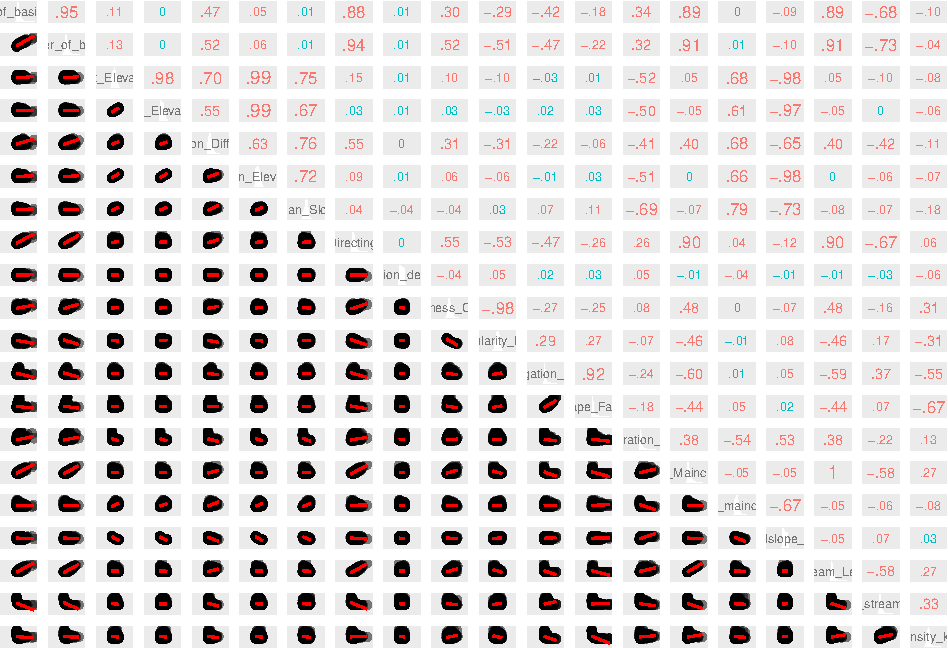
\includegraphics{proyecto_f_files/figure-latex/unnamed-chunk-4-1.pdf}

\begin{verbatim}
##                                          Area_of_basin_km2
## Area_of_basin_km2                             1.0000000000
## Perimeter_of_basin_km                         0.9544758340
## Max_Elevation                                 0.1085164535
## Min_Elevation                                -0.0037333059
## Elevation_Difference                          0.4687069509
## Mean_Elevation                                0.0527159463
## Mean_Slope                                    0.0116722827
## Length_of_Directing_Vector_km                 0.8821719458
## Prevalent_Orientation_deg_from_north_ccw      0.0133206854
## Compactness_Coefficient                       0.3026490133
## Circularity_Ratio                            -0.2885703636
## Elongation_Ratio                             -0.4201325677
## Shape_Factor                                 -0.1774118107
## Concentration_Time_hr                         0.3376141894
## Length_of_Mainchannel_km                      0.8868782573
## Mean_slope_of_mainchannel_percent            -0.0000623078
## Mean_hillslope_length_m                      -0.0868302019
## Total_Stream_Length_km                        0.8866554994
## First_order_stream_frequency                 -0.6765432843
## Drainage_Density_km_over_km2                 -0.0999198137
##                                          Perimeter_of_basin_km
## Area_of_basin_km2                                  0.954475834
## Perimeter_of_basin_km                              1.000000000
## Max_Elevation                                      0.126072976
## Min_Elevation                                      0.003374361
## Elevation_Difference                               0.517032317
## Mean_Elevation                                     0.064253895
## Mean_Slope                                         0.007432527
## Length_of_Directing_Vector_km                      0.941048386
## Prevalent_Orientation_deg_from_north_ccw           0.005013254
## Compactness_Coefficient                            0.524072883
## Circularity_Ratio                                 -0.505511388
## Elongation_Ratio                                  -0.465434321
## Shape_Factor                                      -0.222059361
## Concentration_Time_hr                              0.323183639
## Length_of_Mainchannel_km                           0.912566038
## Mean_slope_of_mainchannel_percent                  0.011612370
## Mean_hillslope_length_m                           -0.097546277
## Total_Stream_Length_km                             0.912065876
## First_order_stream_frequency                      -0.729729329
## Drainage_Density_km_over_km2                      -0.037858082
##                                          Max_Elevation Min_Elevation
## Area_of_basin_km2                          0.108516454  -0.003733306
## Perimeter_of_basin_km                      0.126072976   0.003374361
## Max_Elevation                              1.000000000   0.979845711
## Min_Elevation                              0.979845711   1.000000000
## Elevation_Difference                       0.701703589   0.545241433
## Mean_Elevation                             0.994679678   0.994064553
## Mean_Slope                                 0.750349000   0.669770309
## Length_of_Directing_Vector_km              0.152748940   0.026447839
## Prevalent_Orientation_deg_from_north_ccw   0.008534377   0.011223559
## Compactness_Coefficient                    0.097747484   0.026836115
## Circularity_Ratio                         -0.100979358  -0.030532368
## Elongation_Ratio                          -0.034917788   0.019213707
## Shape_Factor                               0.014803339   0.034733040
## Concentration_Time_hr                     -0.522952456  -0.499344963
## Length_of_Mainchannel_km                   0.050522470  -0.053047221
## Mean_slope_of_mainchannel_percent          0.682330464   0.612424193
## Mean_hillslope_length_m                   -0.976100493  -0.966412179
## Total_Stream_Length_km                     0.050305343  -0.053392624
## First_order_stream_frequency              -0.104632503  -0.004045040
## Drainage_Density_km_over_km2              -0.080209378  -0.063762484
##                                          Elevation_Difference
## Area_of_basin_km2                                 0.468706951
## Perimeter_of_basin_km                             0.517032317
## Max_Elevation                                     0.701703589
## Min_Elevation                                     0.545241433
## Elevation_Difference                              1.000000000
## Mean_Elevation                                    0.628662419
## Mean_Slope                                        0.759984277
## Length_of_Directing_Vector_km                     0.546682345
## Prevalent_Orientation_deg_from_north_ccw         -0.004216387
## Compactness_Coefficient                           0.314482816
## Circularity_Ratio                                -0.314862013
## Elongation_Ratio                                 -0.215062688
## Shape_Factor                                     -0.061759832
## Concentration_Time_hr                            -0.413566386
## Length_of_Mainchannel_km                          0.401222022
## Mean_slope_of_mainchannel_percent                 0.679079570
## Mean_hillslope_length_m                          -0.649322231
## Total_Stream_Length_km                            0.401542793
## First_order_stream_frequency                     -0.424664856
## Drainage_Density_km_over_km2                     -0.109178547
##                                          Mean_Elevation   Mean_Slope
## Area_of_basin_km2                           0.052715946  0.011672283
## Perimeter_of_basin_km                       0.064253895  0.007432527
## Max_Elevation                               0.994679678  0.750349000
## Min_Elevation                               0.994064553  0.669770309
## Elevation_Difference                        0.628662419  0.759984277
## Mean_Elevation                              1.000000000  0.717902080
## Mean_Slope                                  0.717902080  1.000000000
## Length_of_Directing_Vector_km               0.091595925  0.043152236
## Prevalent_Orientation_deg_from_north_ccw    0.008888368 -0.036953776
## Compactness_Coefficient                     0.058377050 -0.039121906
## Circularity_Ratio                          -0.061951571  0.031780506
## Elongation_Ratio                           -0.006958558  0.066886548
## Shape_Factor                                0.026491708  0.109470202
## Concentration_Time_hr                      -0.513112068 -0.688395113
## Length_of_Mainchannel_km                   -0.001812884 -0.074929355
## Mean_slope_of_mainchannel_percent           0.660296508  0.791702711
## Mean_hillslope_length_m                    -0.976432501 -0.725848165
## Total_Stream_Length_km                     -0.002122928 -0.075037094
## First_order_stream_frequency               -0.056487200 -0.070666731
## Drainage_Density_km_over_km2               -0.074394042 -0.178183177
##                                          Length_of_Directing_Vector_km
## Area_of_basin_km2                                           0.88217195
## Perimeter_of_basin_km                                       0.94104839
## Max_Elevation                                               0.15274894
## Min_Elevation                                               0.02644784
## Elevation_Difference                                        0.54668234
## Mean_Elevation                                              0.09159593
## Mean_Slope                                                  0.04315224
## Length_of_Directing_Vector_km                               1.00000000
## Prevalent_Orientation_deg_from_north_ccw                    0.00272695
## Compactness_Coefficient                                     0.54755642
## Circularity_Ratio                                          -0.53162055
## Elongation_Ratio                                           -0.47271463
## Shape_Factor                                               -0.26333595
## Concentration_Time_hr                                       0.26489121
## Length_of_Mainchannel_km                                    0.90154020
## Mean_slope_of_mainchannel_percent                           0.04130672
## Mean_hillslope_length_m                                    -0.12424888
## Total_Stream_Length_km                                      0.90087307
## First_order_stream_frequency                               -0.66625572
## Drainage_Density_km_over_km2                                0.05523891
##                                          Prevalent_Orientation_deg_from_north_ccw
## Area_of_basin_km2                                                     0.013320685
## Perimeter_of_basin_km                                                 0.005013254
## Max_Elevation                                                         0.008534377
## Min_Elevation                                                         0.011223559
## Elevation_Difference                                                 -0.004216387
## Mean_Elevation                                                        0.008888368
## Mean_Slope                                                           -0.036953776
## Length_of_Directing_Vector_km                                         0.002726950
## Prevalent_Orientation_deg_from_north_ccw                              1.000000000
## Compactness_Coefficient                                              -0.038263247
## Circularity_Ratio                                                     0.047959520
## Elongation_Ratio                                                      0.020435968
## Shape_Factor                                                          0.028979551
## Concentration_Time_hr                                                 0.045817442
## Length_of_Mainchannel_km                                             -0.014559540
## Mean_slope_of_mainchannel_percent                                    -0.041954144
## Mean_hillslope_length_m                                              -0.006101928
## Total_Stream_Length_km                                               -0.014834648
## First_order_stream_frequency                                         -0.025730089
## Drainage_Density_km_over_km2                                         -0.062373016
##                                          Compactness_Coefficient
## Area_of_basin_km2                                    0.302649013
## Perimeter_of_basin_km                                0.524072883
## Max_Elevation                                        0.097747484
## Min_Elevation                                        0.026836115
## Elevation_Difference                                 0.314482816
## Mean_Elevation                                       0.058377050
## Mean_Slope                                          -0.039121906
## Length_of_Directing_Vector_km                        0.547556416
## Prevalent_Orientation_deg_from_north_ccw            -0.038263247
## Compactness_Coefficient                              1.000000000
## Circularity_Ratio                                   -0.982893198
## Elongation_Ratio                                    -0.274815245
## Shape_Factor                                        -0.253076546
## Concentration_Time_hr                                0.084829477
## Length_of_Mainchannel_km                             0.477967483
## Mean_slope_of_mainchannel_percent                    0.002602623
## Mean_hillslope_length_m                             -0.074702534
## Total_Stream_Length_km                               0.476467186
## First_order_stream_frequency                        -0.161420996
## Drainage_Density_km_over_km2                         0.310395399
##                                          Circularity_Ratio
## Area_of_basin_km2                             -0.288570364
## Perimeter_of_basin_km                         -0.505511388
## Max_Elevation                                 -0.100979358
## Min_Elevation                                 -0.030532368
## Elevation_Difference                          -0.314862013
## Mean_Elevation                                -0.061951571
## Mean_Slope                                     0.031780506
## Length_of_Directing_Vector_km                 -0.531620546
## Prevalent_Orientation_deg_from_north_ccw       0.047959520
## Compactness_Coefficient                       -0.982893198
## Circularity_Ratio                              1.000000000
## Elongation_Ratio                               0.289513381
## Shape_Factor                                   0.265974071
## Concentration_Time_hr                         -0.074379454
## Length_of_Mainchannel_km                      -0.459171337
## Mean_slope_of_mainchannel_percent             -0.006744063
## Mean_hillslope_length_m                        0.078708721
## Total_Stream_Length_km                        -0.457493385
## First_order_stream_frequency                   0.168318540
## Drainage_Density_km_over_km2                  -0.309107811
##                                          Elongation_Ratio Shape_Factor
## Area_of_basin_km2                            -0.420132568  -0.17741181
## Perimeter_of_basin_km                        -0.465434321  -0.22205936
## Max_Elevation                                -0.034917788   0.01480334
## Min_Elevation                                 0.019213707   0.03473304
## Elevation_Difference                         -0.215062688  -0.06175983
## Mean_Elevation                               -0.006958558   0.02649171
## Mean_Slope                                    0.066886548   0.10947020
## Length_of_Directing_Vector_km                -0.472714634  -0.26333595
## Prevalent_Orientation_deg_from_north_ccw      0.020435968   0.02897955
## Compactness_Coefficient                      -0.274815245  -0.25307655
## Circularity_Ratio                             0.289513381   0.26597407
## Elongation_Ratio                              1.000000000   0.92166632
## Shape_Factor                                  0.921666316   1.00000000
## Concentration_Time_hr                        -0.244967627  -0.18437450
## Length_of_Mainchannel_km                     -0.595756838  -0.43862982
## Mean_slope_of_mainchannel_percent             0.013563039   0.05012741
## Mean_hillslope_length_m                       0.054309895   0.02193559
## Total_Stream_Length_km                       -0.594894045  -0.43777825
## First_order_stream_frequency                  0.370979755   0.06989293
## Drainage_Density_km_over_km2                 -0.546157778  -0.66918169
##                                          Concentration_Time_hr
## Area_of_basin_km2                                   0.33761419
## Perimeter_of_basin_km                               0.32318364
## Max_Elevation                                      -0.52295246
## Min_Elevation                                      -0.49934496
## Elevation_Difference                               -0.41356639
## Mean_Elevation                                     -0.51311207
## Mean_Slope                                         -0.68839511
## Length_of_Directing_Vector_km                       0.26489121
## Prevalent_Orientation_deg_from_north_ccw            0.04581744
## Compactness_Coefficient                             0.08482948
## Circularity_Ratio                                  -0.07437945
## Elongation_Ratio                                   -0.24496763
## Shape_Factor                                       -0.18437450
## Concentration_Time_hr                               1.00000000
## Length_of_Mainchannel_km                            0.37973458
## Mean_slope_of_mainchannel_percent                  -0.54157779
## Mean_hillslope_length_m                             0.53319066
## Total_Stream_Length_km                              0.37928755
## First_order_stream_frequency                       -0.22050640
## Drainage_Density_km_over_km2                        0.12574975
##                                          Length_of_Mainchannel_km
## Area_of_basin_km2                                     0.886878257
## Perimeter_of_basin_km                                 0.912566038
## Max_Elevation                                         0.050522470
## Min_Elevation                                        -0.053047221
## Elevation_Difference                                  0.401222022
## Mean_Elevation                                       -0.001812884
## Mean_Slope                                           -0.074929355
## Length_of_Directing_Vector_km                         0.901540197
## Prevalent_Orientation_deg_from_north_ccw             -0.014559540
## Compactness_Coefficient                               0.477967483
## Circularity_Ratio                                    -0.459171337
## Elongation_Ratio                                     -0.595756838
## Shape_Factor                                         -0.438629821
## Concentration_Time_hr                                 0.379734584
## Length_of_Mainchannel_km                              1.000000000
## Mean_slope_of_mainchannel_percent                    -0.048088478
## Mean_hillslope_length_m                              -0.053644883
## Total_Stream_Length_km                                0.999712141
## First_order_stream_frequency                         -0.577404672
## Drainage_Density_km_over_km2                          0.273665370
##                                          Mean_slope_of_mainchannel_percent
## Area_of_basin_km2                                            -0.0000623078
## Perimeter_of_basin_km                                         0.0116123695
## Max_Elevation                                                 0.6823304637
## Min_Elevation                                                 0.6124241933
## Elevation_Difference                                          0.6790795702
## Mean_Elevation                                                0.6602965081
## Mean_Slope                                                    0.7917027108
## Length_of_Directing_Vector_km                                 0.0413067240
## Prevalent_Orientation_deg_from_north_ccw                     -0.0419541444
## Compactness_Coefficient                                       0.0026026227
## Circularity_Ratio                                            -0.0067440632
## Elongation_Ratio                                              0.0135630387
## Shape_Factor                                                  0.0501274147
## Concentration_Time_hr                                        -0.5415777885
## Length_of_Mainchannel_km                                     -0.0480884780
## Mean_slope_of_mainchannel_percent                             1.0000000000
## Mean_hillslope_length_m                                      -0.6681192684
## Total_Stream_Length_km                                       -0.0474631511
## First_order_stream_frequency                                 -0.0557148988
## Drainage_Density_km_over_km2                                 -0.0801406065
##                                          Mean_hillslope_length_m
## Area_of_basin_km2                                   -0.086830202
## Perimeter_of_basin_km                               -0.097546277
## Max_Elevation                                       -0.976100493
## Min_Elevation                                       -0.966412179
## Elevation_Difference                                -0.649322231
## Mean_Elevation                                      -0.976432501
## Mean_Slope                                          -0.725848165
## Length_of_Directing_Vector_km                       -0.124248878
## Prevalent_Orientation_deg_from_north_ccw            -0.006101928
## Compactness_Coefficient                             -0.074702534
## Circularity_Ratio                                    0.078708721
## Elongation_Ratio                                     0.054309895
## Shape_Factor                                         0.021935590
## Concentration_Time_hr                                0.533190662
## Length_of_Mainchannel_km                            -0.053644883
## Mean_slope_of_mainchannel_percent                   -0.668119268
## Mean_hillslope_length_m                              1.000000000
## Total_Stream_Length_km                              -0.053467451
## First_order_stream_frequency                         0.068526699
## Drainage_Density_km_over_km2                         0.027552614
##                                          Total_Stream_Length_km
## Area_of_basin_km2                                   0.886655499
## Perimeter_of_basin_km                               0.912065876
## Max_Elevation                                       0.050305343
## Min_Elevation                                      -0.053392624
## Elevation_Difference                                0.401542793
## Mean_Elevation                                     -0.002122928
## Mean_Slope                                         -0.075037094
## Length_of_Directing_Vector_km                       0.900873075
## Prevalent_Orientation_deg_from_north_ccw           -0.014834648
## Compactness_Coefficient                             0.476467186
## Circularity_Ratio                                  -0.457493385
## Elongation_Ratio                                   -0.594894045
## Shape_Factor                                       -0.437778253
## Concentration_Time_hr                               0.379287551
## Length_of_Mainchannel_km                            0.999712141
## Mean_slope_of_mainchannel_percent                  -0.047463151
## Mean_hillslope_length_m                            -0.053467451
## Total_Stream_Length_km                              1.000000000
## First_order_stream_frequency                       -0.577169211
## Drainage_Density_km_over_km2                        0.274631240
##                                          First_order_stream_frequency
## Area_of_basin_km2                                         -0.67654328
## Perimeter_of_basin_km                                     -0.72972933
## Max_Elevation                                             -0.10463250
## Min_Elevation                                             -0.00404504
## Elevation_Difference                                      -0.42466486
## Mean_Elevation                                            -0.05648720
## Mean_Slope                                                -0.07066673
## Length_of_Directing_Vector_km                             -0.66625572
## Prevalent_Orientation_deg_from_north_ccw                  -0.02573009
## Compactness_Coefficient                                   -0.16142100
## Circularity_Ratio                                          0.16831854
## Elongation_Ratio                                           0.37097976
## Shape_Factor                                               0.06989293
## Concentration_Time_hr                                     -0.22050640
## Length_of_Mainchannel_km                                  -0.57740467
## Mean_slope_of_mainchannel_percent                         -0.05571490
## Mean_hillslope_length_m                                    0.06852670
## Total_Stream_Length_km                                    -0.57716921
## First_order_stream_frequency                               1.00000000
## Drainage_Density_km_over_km2                               0.33133675
##                                          Drainage_Density_km_over_km2
## Area_of_basin_km2                                         -0.09991981
## Perimeter_of_basin_km                                     -0.03785808
## Max_Elevation                                             -0.08020938
## Min_Elevation                                             -0.06376248
## Elevation_Difference                                      -0.10917855
## Mean_Elevation                                            -0.07439404
## Mean_Slope                                                -0.17818318
## Length_of_Directing_Vector_km                              0.05523891
## Prevalent_Orientation_deg_from_north_ccw                  -0.06237302
## Compactness_Coefficient                                    0.31039540
## Circularity_Ratio                                         -0.30910781
## Elongation_Ratio                                          -0.54615778
## Shape_Factor                                              -0.66918169
## Concentration_Time_hr                                      0.12574975
## Length_of_Mainchannel_km                                   0.27366537
## Mean_slope_of_mainchannel_percent                         -0.08014061
## Mean_hillslope_length_m                                    0.02755261
## Total_Stream_Length_km                                     0.27463124
## First_order_stream_frequency                               0.33133675
## Drainage_Density_km_over_km2                               1.00000000
\end{verbatim}

El análisis de correlación entre la variable dependiente seleccionada
(Densidad de Drenaje) y las demás sometidas a prueba, resultaron con
índice mayor a 0.5 factor de forma (-0.669485228) y ratio de elongación
(-0.545994239). Para dar mayor robustez al modelo que se diseñó, se
incorporaron las variables: pendiente promedio (-0.176066777) y longitud
total del curso principal medido en km (0.274832295).

\textbf{Comprobación del supuesto de distribución normal de las
observaciones de las variables analizadas}

La comprobación del supuesto de normalidad se hizo mediante el gráfico
cuantilar de las variables donde se incluyó el ajuste logarítmico de la
variable dependiente a consecuencia del sesgo evidenciado ya que se
puede tolerar la no distribución normal de las independientes, no así en
la dependiente.

\includegraphics{proyecto_f_files/figure-latex/unnamed-chunk-6-1.pdf}

\textbf{Estadística cuantilar de variables utilizadas}

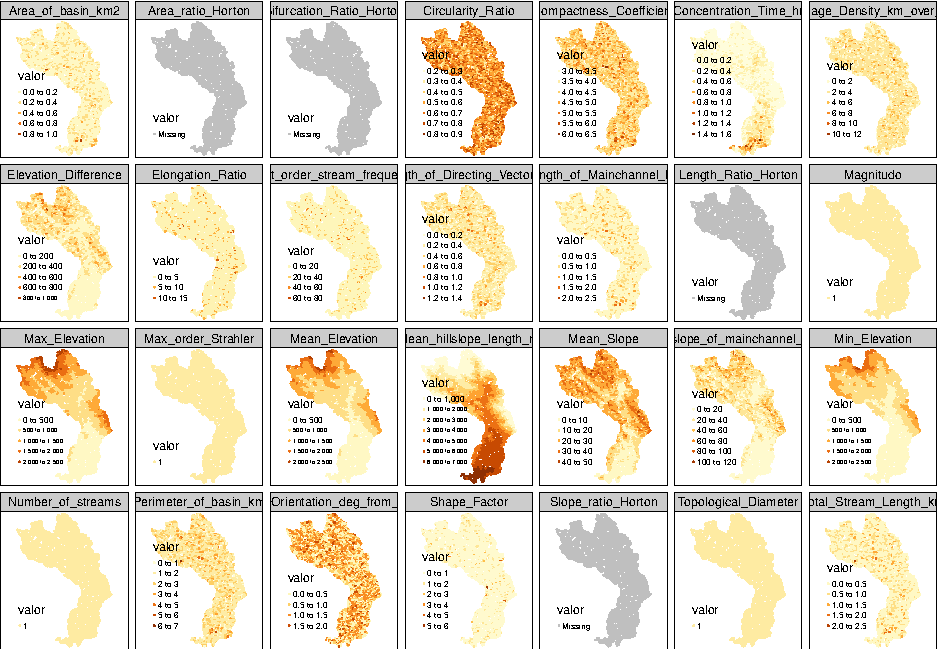
\includegraphics{proyecto_f_files/figure-latex/unnamed-chunk-7-1.pdf}

Se asume como válido el supuesto de normalidad de los datos tanto en el
diagrama cuantilar normal en el cual se muestra un relativo acercamiento
de los puntos a una forma de la recta que representan las observaciones
de cada una de las variables analizadas, como los indicadores numéricos
de la prueba de Shapiro-Wilk con ``p'' menores a 0.05, indicando
significancia y que se cumple el supuesto de distribución normal de los
datos de las variables analizadas.

\textbf{Seleccion de variable dependiente Densidad de Drenaje}

\begin{verbatim}
## Warning: funs() is soft deprecated as of dplyr 0.8.0
## Please use a list of either functions or lambdas: 
## 
##   # Simple named list: 
##   list(mean = mean, median = median)
## 
##   # Auto named with `tibble::lst()`: 
##   tibble::lst(mean, median)
## 
##   # Using lambdas
##   list(~ mean(., trim = .2), ~ median(., na.rm = TRUE))
## This warning is displayed once per session.
\end{verbatim}

\begin{verbatim}
## Warning in log(round(logDD/DD, 4) * 100): NaNs produced
\end{verbatim}

\begin{verbatim}
## Simple feature collection with 3027 features and 30 fields
## geometry type:  POLYGON
## dimension:      XY
## bbox:           xmin: 317400 ymin: 2019180 xmax: 352260 ymax: 2067690
## epsg (SRID):    32619
## proj4string:    +proj=utm +zone=19 +datum=WGS84 +units=m +no_defs
## First 10 features:
##        fid cat value label       DD        SF        ER     TS    MS
## 1  3.0e+09   2     1       2.189137 0.4974215 1.1522986 0.5194 26.44
## 2  4.0e+09   3     3       1.317045 1.5193957 6.7526210 0.0849 31.26
## 3  5.0e+09   7     2       5.021898 0.2158705 0.8774590 0.3870 24.12
## 4  6.0e+09  11    18       3.348350 0.3116489 0.7588246 0.7191 27.12
## 5  7.0e+09   8     8       1.323741 0.9530676 3.2504695 0.1449 36.98
## 6  8.0e+09   9     4       5.407681 0.2022916 0.7547642 0.4946 23.41
## 7  9.0e+09  12    10       1.707515 0.6384885 1.5645024 0.3621 34.67
## 8  1.0e+10  14     9       1.776552 0.7101480 2.8058127 0.1449 37.30
## 9  1.1e+10  15    14       1.017378 1.2400654 3.7077166 0.1449 37.36
## 10 1.2e+10  10    13       1.376470 0.8268738 2.2012308 0.2473 30.57
##        logDD        x       y                       geometry value_PCT
## 1  0.7835072 334063.9 2067449 POLYGON ((334500 2067660, 3...     45.68
## 2  0.2753904 334582.9 2067514 POLYGON ((334500 2067390, 3...    227.78
## 3  1.6138079 334172.4 2067265 POLYGON ((334440 2067330, 3...     39.83
## 4  1.2084677 334366.4 2066754 POLYGON ((333840 2067180, 3...    537.58
## 5  0.2804618 333919.7 2066981 POLYGON ((333750 2067240, 3...    604.35
## 6  1.6878203 334365.9 2067039 POLYGON ((334380 2067240, 3...     73.97
## 7  0.5350394 333028.9 2066963 POLYGON ((332640 2067120, 3...    585.65
## 8  0.5746743 333771.9 2066901 POLYGON ((333540 2067090, 3...    506.60
## 9  0.0172283 333384.3 2066840 POLYGON ((333330 2067090, 3...   1376.09
## 10 0.3195221 332580.6 2066931 POLYGON ((332280 2067000, 3...    944.45
##    DD_PCT SF_PCT ER_PCT TS_PCT  MS_PCT logDD_PCT    x_PCT     y_PCT
## 1     100  22.72  52.64  23.73 1207.78     35.79 15260075  94441321
## 2     100 115.36 512.71   6.45 2373.50     20.91 25404065 156981278
## 3     100   4.30  17.47   7.71  480.30     32.14  6654306  41165011
## 4     100   9.31  22.66  21.48  809.95     36.09  9986005  61724553
## 5     100  72.00 245.55  10.95 2793.60     21.19 25225453 156146939
## 6     100   3.74  13.96   9.15  432.90     31.21  6183166  38224128
## 7     100  37.39  91.62  21.21 2030.44     31.33 19503709 121050909
## 8     100  39.97 157.94   8.16 2099.57     32.35 18787628 116343433
## 9     100 121.89 364.44  14.24 3672.19      1.69 32768985 203153658
## 10    100  60.07 159.92  17.97 2220.90     23.21 24161853 150161743
##    value_PCTLOG DD_PCTLOG SF_PCTLOG ER_PCTLOG TS_PCTLOG MS_PCTLOG
## 1      3.821661   4.60517  3.123246  3.963476  3.166740  7.096539
## 2      5.428380   4.60517  4.748058  6.239710  1.864080  7.772121
## 3      3.684620   4.60517  1.458615  2.860485  2.042518  6.174411
## 4      6.287078   4.60517  2.231089  3.120601  3.067122  6.696973
## 5      6.404154   4.60517  4.276666  5.503501  2.393339  7.935086
## 6      4.303660   4.60517  1.319086  2.636196  2.213754  6.070507
## 7      6.372722   4.60517  3.621403  4.517650  3.054473  7.616008
## 8      6.227722   4.60517  3.688129  5.062215  2.099244  7.649488
## 9      7.227001   4.60517  4.803119  5.898362  2.656055  8.208543
## 10     6.850603   4.60517  4.095511  5.074674  2.888704  7.705668
##    logDD_PCTLOG x_PCTLOG y_PCTLOG
## 1     3.5776685 16.54075 18.36349
## 2     3.0402275 17.05042 18.87164
## 3     3.4701014 15.71077 17.53310
## 4     3.5860158 16.11670 17.93819
## 5     3.0535294 17.04336 18.86631
## 6     3.4407386 15.63734 17.45898
## 7     3.4445761 16.78612 18.61172
## 8     3.4766140 16.74871 18.57206
## 9     0.5247285 17.30499 19.12947
## 10    3.1445832 17.00029 18.82722
\end{verbatim}

\includegraphics{proyecto_f_files/figure-latex/unnamed-chunk-11-1.pdf}

\textbf{Comprobación de supuesto de autocorrelación de la variable
dependiente transformada (I de Moran Global).}

Visualización porcentual de la dispersión de la Variable seleccionada
Densidad de Drenaje ajustada logarítmicamente en cuatro cuadrantes.

\textbf{Diagrama Dispersión G. Moran}

\begin{verbatim}
## Characteristics of weights list object:
## Neighbour list object:
## Number of regions: 3027 
## Number of nonzero links: 15135 
## Percentage nonzero weights: 0.16518 
## Average number of links: 5 
## Non-symmetric neighbours list
## 
## Weights style: W 
## Weights constants summary:
##      n      nn   S0      S1       S2
## W 3027 9162729 3027 1111.88 12356.64
\end{verbatim}

\textbf{Diagrama de Dispersión Moran PesoW}

\includegraphics{proyecto_f_files/figure-latex/unnamed-chunk-14-1.pdf}

\begin{verbatim}
## 
##  Moran I test under randomisation
## 
## data:  log1p(datos$Drainage_Density_km_over_km2)  
## weights: PesoW    
## 
## Moran I statistic standard deviate = -1.2064, p-value = 0.8862
## alternative hypothesis: greater
## sample estimates:
## Moran I statistic       Expectation          Variance 
##     -0.0136063144     -0.0003304693      0.0001210999
\end{verbatim}

Se acepta preliminarmente la hipótesis nula la cual sostiene que
\textbf{NO} hay autocorrelación espacial dado un valor de ``p''
\textgreater{} 0.05 (0.8862).

\textbf{Variable dependiente original DD y ajustada logDD}

\includegraphics{proyecto_f_files/figure-latex/unnamed-chunk-16-1.pdf}

\textbf{Evaluación de la autocorrelación espacial local de la variable
dependiente transformada}

La aparición de parches rojos y azules indican la existencia de
autocorrelación local. Los parches rojos traducen hotspots o altos
valores de correlación. Los parches azules traducen coldspots e indican
autocorrelación con valores bajos. Finalmente, los valores grises
indican ausencia de correlación local.

\textbf{Análisis de vecindad por contigüidad (vecxcont)}

Resultaron 3027 regiones ya que cada observación en este caso funge como
una unidad espacial independiente. La prueba de peso homogéneo de
vecindad arrojó 5760 conexiones distintas de cero con un promedio de
conexiones de 1.901618 para un valor porcentual de 6.28\%, dos regiones
con 9 conexiones y 695 regiones sin conexión alguna.

\textbf{Análisis de Vecindad por cantidad de los 5 vecinos más cercanos}

Los valores de la data completa y la de los 5 vecinos más cercanos ya
que cada observación corresponde a una unidad espacial, es decir,
absolutamente todas las observaciones son vecinos entre si (In
knearneigh(coords, k=5) : knearneigh: identical points found).

\textbf{Análisis de Vecindad por peso de observaciones vecinas en
Varselpol3}

Por tratarse de un espacio geográfico limitado cuyas unidades espaciales
(microcuencas) corresponden a las mismas observaciones puntuales, los
valores de conexiones y vecindades no difieren mucho en las diferentes
combinaciones de vecindad examinadas. En este caso el número de regiones
sigue siendo 3027. Las conexiones diferentes de cero son 15145, el
porcentaje de conexiones no cero es 16.5\% y el promedio de conexiones
es de 5.

\section{MODELIZACION}\label{modelizacion}

Visualización porcentual de la dispersión de la Variable seleccionada
Densidad de Drenaje ajustada logarítmicamente en cuatro cuadrantes

\includegraphics{proyecto_f_files/figure-latex/unnamed-chunk-21-1.pdf}

\textbf{Comprobación del Supuesto de Autocorrelación mediante la Prueba
de Moran Global:}

El valor de ``p'' es mayor a 0.05 (valor comunmente establecido), se
acepta la hipotesis nula ``No hay autocorrelación espacial global'' con
sus vecinos en la variable dependiente en su versión original. Aunque el
sistema de cuenta de la aceptación de la misma (alternative hyphotesis:
greater).

\begin{verbatim}
## 
##  Moran I test under randomisation
## 
## data:  log1p(datos$Drainage_Density_km_over_km2)  
## weights: PesowB    
## 
## Moran I statistic standard deviate = -1.2064, p-value = 0.8862
## alternative hypothesis: greater
## sample estimates:
## Moran I statistic       Expectation          Variance 
##     -0.0136063144     -0.0003304693      0.0001210999
\end{verbatim}

\begin{verbatim}
## 
##  Moran I test under randomisation
## 
## data:  Varselpctlog$logDD_PCT  
## weights: PesowB    
## 
## Moran I statistic standard deviate = -0.20036, p-value = 0.5794
## alternative hypothesis: greater
## sample estimates:
## Moran I statistic       Expectation          Variance 
##     -0.0024973085     -0.0003304693      0.0001169561
\end{verbatim}

En el caso de la prueba de los supuestos de autocorrelación de la
variable tanto por contigüidad como por peso coinciden por la misma
causa que en el análisis de vecindad en entidades poligonales, las
unidades espaciales (microcuencas) son los mismos puntos de observación,
es decir, tenemos tantos modelos como puntos de observación en el
análisis.

\textbf{Hipotesis alternativa}

El valor de ``p'' es menor a 0.05 (valor comunmente establecido), se
rechaza la hipótesis nula ``No hay autocorrelación espacial global'' con
sus vecinos respecto a la variable porcentual ajustada por logaritmo.

\textbf{Correlación de Moral local de la variable Logarítmica}

\textbf{Comprobación del supuesto de normalidad (shapiro-wilk)}

\begin{verbatim}
## 
##  Shapiro-Wilk normality test
## 
## data:  Varselpctlog$logDD_PCT
## W = 0.33179, p-value < 2.2e-16
\end{verbatim}

El valor de ``p'' es menor a 0.05 (2.2e-16), se rechaza la hipotesis
nula ``No hay distribución normal'' , en otras palabras se acepta la
hipotesis alternativa ``Existe distribución normal de las observaciones
de la variable analizada(Varselpctlog\$logDD\_PCT)''.

\begin{verbatim}
## 
##  Shapiro-Wilk normality test
## 
## data:  Varselpctlog$logDD_PCTLOG
## W = 0.37252, p-value < 2.2e-16
\end{verbatim}

El valor de ``p'' es menor a 0.05 (2.2e-16), se rechaza la hipotesis
nula ``No hay distribución normal'' , en otras palabras se acepta la
hipotesis alternativa ``Existe distribución normal de las observaciones
de la variable analizada(Varselpctlog\$logDD\_PCTLOG)''. En sisntesis,
se cumple el supuesto de normalidad en ambas versiones de la variable
dependiente del modelo analizado.

\textbf{Comprobación de supuesto de heterocedasticidad (prueba de
Breusch-Pagan)}

\begin{verbatim}
## 
## Call:
## lm(formula = logDD ~ ., data = .)
## 
## Residuals:
##      Min       1Q   Median       3Q      Max 
## -0.48090 -0.13441 -0.03593  0.08960  2.48258 
## 
## Coefficients:
##               Estimate Std. Error t value Pr(>|t|)    
## (Intercept)  1.3355070  0.0139626  95.649  < 2e-16 ***
## TS           0.2364021  0.0194249  12.170  < 2e-16 ***
## MS          -0.0027199  0.0003979  -6.835 9.85e-12 ***
## SF          -1.3103680  0.0240590 -54.465  < 2e-16 ***
## ER           0.1482183  0.0062693  23.642  < 2e-16 ***
## ---
## Signif. codes:  0 '***' 0.001 '**' 0.01 '*' 0.05 '.' 0.1 ' ' 1
## 
## Residual standard error: 0.2045 on 3022 degrees of freedom
## Multiple R-squared:  0.7511, Adjusted R-squared:  0.7507 
## F-statistic:  2279 on 4 and 3022 DF,  p-value: < 2.2e-16
\end{verbatim}

\begin{verbatim}
## 
## Call:
## lm(formula = logDD_PCTLOG ~ ., data = .)
## 
## Residuals:
##     Min      1Q  Median      3Q     Max 
## -5.8010 -0.0488  0.0511  0.1056  0.4639 
## 
## Coefficients: (1 not defined because of singularities)
##               Estimate Std. Error t value Pr(>|t|)   
## (Intercept)   2.333195  32.050951   0.073  0.94197   
## value_PCTLOG  0.016642   0.006338   2.626  0.00869 **
## DD_PCTLOG           NA         NA      NA       NA   
## SF_PCTLOG     3.054474  13.128693   0.233  0.81604   
## ER_PCTLOG    -3.523054  13.124042  -0.268  0.78838   
## TS_PCTLOG    -1.779470   6.562320  -0.271  0.78628   
## MS_PCTLOG     0.010921   0.007138   1.530  0.12612   
## x_PCTLOG      0.080123   0.226237   0.354  0.72325   
## y_PCTLOG      0.524177   0.256973   2.040  0.04146 * 
## ---
## Signif. codes:  0 '***' 0.001 '**' 0.01 '*' 0.05 '.' 0.1 ' ' 1
## 
## Residual standard error: 0.2652 on 2949 degrees of freedom
##   (70 observations deleted due to missingness)
## Multiple R-squared:  0.2786, Adjusted R-squared:  0.2769 
## F-statistic: 162.7 on 7 and 2949 DF,  p-value: < 2.2e-16
\end{verbatim}

\begin{verbatim}
## 
##  studentized Breusch-Pagan test
## 
## data:  .
## BP = 83.112, df = 7, p-value = 3.189e-15
\end{verbatim}

El valor de ``p'' es menor a 0.05 (3.189e-15), en la prueba de
Breuch-Pagan tiene como hipótesis nula ``Hay homocedasticidad'', en
otras palabras se acepta la hipotesis alternativa ``Existe
heterocedasticidad'' las observaciones de las variables analizadas en el
modelo lineal con la versión de ajuste logaritmico de la variable
dependiente.

\subsection{Análisis del modelo
lineal**}\label{anuxe1lisis-del-modelo-lineal}

\begin{verbatim}
## 
## Call:
## lm(formula = logDD ~ ., data = .)
## 
## Residuals:
##      Min       1Q   Median       3Q      Max 
## -0.48090 -0.13441 -0.03593  0.08960  2.48258 
## 
## Coefficients:
##               Estimate Std. Error t value Pr(>|t|)    
## (Intercept)  1.3355070  0.0139626  95.649  < 2e-16 ***
## TS           0.2364021  0.0194249  12.170  < 2e-16 ***
## MS          -0.0027199  0.0003979  -6.835 9.85e-12 ***
## SF          -1.3103680  0.0240590 -54.465  < 2e-16 ***
## ER           0.1482183  0.0062693  23.642  < 2e-16 ***
## ---
## Signif. codes:  0 '***' 0.001 '**' 0.01 '*' 0.05 '.' 0.1 ' ' 1
## 
## Residual standard error: 0.2045 on 3022 degrees of freedom
## Multiple R-squared:  0.7511, Adjusted R-squared:  0.7507 
## F-statistic:  2279 on 4 and 3022 DF,  p-value: < 2.2e-16
\end{verbatim}

Todos los coeficientes de las variables del modelo han resultado
signicativas (p\textless{}0.05) y el R cuadrado ajustado del modelo
indica que las variables independientes analizadas explican en un
75.07\% a la variable dependiente Dendidad de drenaje. Por otro lado, si
el valor de las independientes fuera cero, la variable dependiente
tomaria el valor 1.3355070 (intercepto).

Las demás pruebas correspondientes al mismo modelo lineal utilizando
versiones transformadas de las valiables(\% y Log e) resultaron no
significativos, es decir, las variables independientes analizadas no
logran explicar el comportamiento de la variable dependiente, en tanto,
no resultan útiles para la predicción de escenarios de la Densidad de
Drenaje de la cuenca del Río Ocoa.

\section{Modelo lineal común, utilizando las versiones transformadas de
las
variables}\label{modelo-lineal-comuxfan-utilizando-las-versiones-transformadas-de-las-variables}

\begin{verbatim}
## 
## Call:
## lm(formula = logDD_PCTLOG ~ ., data = .)
## 
## Residuals:
##     Min      1Q  Median      3Q     Max 
## -5.8010 -0.0488  0.0511  0.1056  0.4639 
## 
## Coefficients: (1 not defined because of singularities)
##               Estimate Std. Error t value Pr(>|t|)   
## (Intercept)   2.333195  32.050951   0.073  0.94197   
## value_PCTLOG  0.016642   0.006338   2.626  0.00869 **
## DD_PCTLOG           NA         NA      NA       NA   
## SF_PCTLOG     3.054474  13.128693   0.233  0.81604   
## ER_PCTLOG    -3.523054  13.124042  -0.268  0.78838   
## TS_PCTLOG    -1.779470   6.562320  -0.271  0.78628   
## MS_PCTLOG     0.010921   0.007138   1.530  0.12612   
## x_PCTLOG      0.080123   0.226237   0.354  0.72325   
## y_PCTLOG      0.524177   0.256973   2.040  0.04146 * 
## ---
## Signif. codes:  0 '***' 0.001 '**' 0.01 '*' 0.05 '.' 0.1 ' ' 1
## 
## Residual standard error: 0.2652 on 2949 degrees of freedom
##   (70 observations deleted due to missingness)
## Multiple R-squared:  0.2786, Adjusted R-squared:  0.2769 
## F-statistic: 162.7 on 7 and 2949 DF,  p-value: < 2.2e-16
\end{verbatim}

\textbf{Prueba de Breush Pagan del modelo lineal la variable logarítmica
transformada}

\begin{verbatim}
## 
##  studentized Breusch-Pagan test
## 
## data:  .
## BP = 83.112, df = 7, p-value = 3.189e-15
\end{verbatim}

\section{Análisis del modelo espacial autoregresivo
(SAR)}\label{anuxe1lisis-del-modelo-espacial-autoregresivo-sar}

\begin{verbatim}
## 
## Call: spautolm(formula = logDD_PCTLOG ~ ., data = ., listw = PesoW)
## 
## Residuals:
##       Min        1Q    Median        3Q       Max 
## -5.788417 -0.048925  0.051674  0.106056  0.469856 
## 
## Coefficients: 
##     (1 not defined because of singularities)
##                Estimate Std. Error z value Pr(>|z|)
## (Intercept)   1.9044081 31.9519406  0.0596  0.95247
## value_PCTLOG  0.0162723  0.0066833  2.4348  0.01490
## DD_PCTLOG            NA         NA      NA       NA
## SF_PCTLOG     2.8840633 13.0874847  0.2204  0.82558
## ER_PCTLOG    -3.3535908 13.0828255 -0.2563  0.79769
## TS_PCTLOG    -1.6955321  6.5417008 -0.2592  0.79549
## MS_PCTLOG     0.0110922  0.0074381  1.4913  0.13589
## x_PCTLOG      0.0857658  0.2387982  0.3592  0.71948
## y_PCTLOG      0.5205009  0.2677977  1.9436  0.05194
## 
## Lambda: 0.055236 LR test value: 3.4252 p-value: 0.064209 
## Numerical Hessian standard error of lambda: 0.040136 
## 
## Log likelihood: -265.6079 
## ML residual variance (sigma squared): 0.070035, (sigma: 0.26464)
## Number of observations: 2957 
## Number of parameters estimated: 10 
## AIC: 551.22
\end{verbatim}

\subsection{Análisis del modelo espacial autoregresivo (SAR) con el
porcentaje logarítimico de las variables con radio de
elongación}\label{anuxe1lisis-del-modelo-espacial-autoregresivo-sar-con-el-porcentaje-logaruxedtimico-de-las-variables-con-radio-de-elongaciuxf3n}

\begin{verbatim}
## 
## Call: 
## spautolm(formula = logDD_PCTLOG ~ TS_PCTLOG + MS_PCTLOG + SF_PCTLOG + 
##     ER_PCTLOG, data = ., listw = PesoW)
## 
## Residuals:
##       Min        1Q    Median        3Q       Max 
## -5.804683 -0.054166  0.053495  0.120415  0.371207 
## 
## Coefficients: 
##               Estimate Std. Error z value Pr(>|z|)
## (Intercept) 27.7761803 31.7597450  0.8746   0.3818
## TS_PCTLOG   -4.8872312  6.5529974 -0.7458   0.4558
## MS_PCTLOG    0.0094571  0.0066620  1.4195   0.1557
## SF_PCTLOG    9.6571365 13.1034848  0.7370   0.4611
## ER_PCTLOG   -9.8523852 13.1034913 -0.7519   0.4521
## 
## Lambda: 0.06329 LR test value: 4.5485 p-value: 0.032948 
## Numerical Hessian standard error of lambda: 0.029943 
## 
## Log likelihood: -282.6669 
## ML residual variance (sigma squared): 0.070836, (sigma: 0.26615)
## Number of observations: 2957 
## Number of parameters estimated: 7 
## AIC: 579.33
\end{verbatim}

Ninguna de las variables independientes resultó significativa (todos los
Pr resultaron mayores de 0.05) para explicar la variable dependiente.

\subsection{Análisis del modelo espacial autoregresivo (SAR) con las
variables de porcentaje logarítimico sin radio de
elongación}\label{anuxe1lisis-del-modelo-espacial-autoregresivo-sar-con-las-variables-de-porcentaje-logaruxedtimico-sin-radio-de-elongaciuxf3n}

\begin{verbatim}
## 
## Call: 
## spautolm(formula = logDD_PCTLOG ~ TS_PCTLOG + MS_PCTLOG + SF_PCTLOG, 
##     data = ., listw = PesoW)
## 
## Residuals:
##       Min        1Q    Median        3Q       Max 
## -5.806072 -0.053655  0.054242  0.120115  0.367763 
## 
## Coefficients: 
##               Estimate Std. Error  z value  Pr(>|z|)
## (Intercept)  3.8963547  0.0389584 100.0132 < 2.2e-16
## TS_PCTLOG    0.0398969  0.0077097   5.1749 2.281e-07
## MS_PCTLOG    0.0095269  0.0066632   1.4298    0.1528
## SF_PCTLOG   -0.1952446  0.0069732 -27.9991 < 2.2e-16
## 
## Lambda: 0.063486 LR test value: 4.5767 p-value: 0.03241 
## Numerical Hessian standard error of lambda: 0.029449 
## 
## Log likelihood: -282.9495 
## ML residual variance (sigma squared): 0.070849, (sigma: 0.26617)
## Number of observations: 2957 
## Number of parameters estimated: 6 
## AIC: 577.9
\end{verbatim}

Solo la variable mean slope en su versión porcentual logarítmica
(MA\_PCTLOG) no es significativa para explicar la variable dependiente
(Pr\textgreater{}0.05), adicionalmente la variable independiente
\texttt{factor} de forma (SF\_PCTLOG) presenta correlación negativa o
inversa sobre la densidad de drenaje (-0.1952446). En ambos modelos SAR,
el AIC (akaike information criterion) resultó significativamente alto,
ya que debe ser cercano a cero.

\section{GEOESTADISTICA Y DATOS
PUNTUALES}\label{geoestadistica-y-datos-puntuales}

\subsection{Kriging}\label{kriging}

El kriging es un método geoestadístico basado en la teoría de variables
regionalizadas. Consiste en establecer la interpolación óptima entre los
puntos de un interpolador local a la vez que cumple con los supuestos
resaltados por Olaya (2011), en el caso de kriging ordinario:

\begin{enumerate}
\def\labelenumi{\arabic{enumi}.}
\tightlist
\item
  Normalidad de la distribución de los datos de la variable interpolada
\item
  Media y varianza constantes a lo largo del área interpolada.
\item
  Covarianza solo en dependencia de la distancia entre puntos.
\item
  Autocorrelación significativa
\item
  Error mínimo de predicción
\item
  Pesos cercanos mayores que los lejanos
\item
  La presencia de un punto cercano en una dirección dada debe restar
  influencia a puntos en la misma dirección, pero más lejanos.
\item
  Puntos muy cercanos con valores muy similares deben agruparse de forma
  que no aparezca sesgo por sobre muestreo.
\item
  La estimación del error debe hacerse en función de la estructura de
  los puntos (ubicación), no de los valores.
\end{enumerate}

El primer paso para iniciar la interpolación es la definición del
sistema de coordenadas destino para nuestro modelo, en nuestro caso
usaremos WGS84 UTM Zona 19 (EPSG:32619) como se había mencionado
anteriormente.

Creamos el objeto \texttt{orden1logdd} que es el resultado de la
variable transformada \texttt{logDD}.

Luego creamos el objeto \texttt{v} para representar el variograma.

\begin{Shaded}
\begin{Highlighting}[]
\KeywordTok{plot}\NormalTok{(v)}
\end{Highlighting}
\end{Shaded}

\includegraphics{proyecto_f_files/figure-latex/unnamed-chunk-45-1.pdf}

Después de tener nuestro objeto creado para representar el variograma,
prodecedimos a la creación de los variogramas modelo esférico,
exponencial y gauseano.

\textbf{Variograma Modelo Esférico}

\begin{Shaded}
\begin{Highlighting}[]
\KeywordTok{plot}\NormalTok{(v, v_m)}
\end{Highlighting}
\end{Shaded}

\includegraphics{proyecto_f_files/figure-latex/unnamed-chunk-47-1.pdf}

\textbf{Variograma Modelo Exponencial}

\begin{Shaded}
\begin{Highlighting}[]
\KeywordTok{plot}\NormalTok{(v, v_m2)}
\end{Highlighting}
\end{Shaded}

\includegraphics{proyecto_f_files/figure-latex/unnamed-chunk-49-1.pdf}

\textbf{Variograma Modelo Gauseano}

\begin{Shaded}
\begin{Highlighting}[]
\KeywordTok{plot}\NormalTok{(v, v_m)}
\end{Highlighting}
\end{Shaded}

\includegraphics{proyecto_f_files/figure-latex/unnamed-chunk-51-1.pdf}

Podemos notar que los variogramas generados no presentan un patrón
autocorrelacionado significativo, puesto que la semivarianza no aumenta
gradualmente, de acuerdo al supuesto de autorrelacion significativo.

En este sentido, procedimos a la verificación de error de predicción de
variogramas para elegir el que tenga menos error.

\begin{Shaded}
\begin{Highlighting}[]
\KeywordTok{attr}\NormalTok{(v_m, }\StringTok{'SSErr'}\NormalTok{) }\CommentTok{# Esférico}
\end{Highlighting}
\end{Shaded}

\begin{verbatim}
## [1] 2.496814e-07
\end{verbatim}

\begin{Shaded}
\begin{Highlighting}[]
\KeywordTok{attr}\NormalTok{(v_m2, }\StringTok{'SSErr'}\NormalTok{) }\CommentTok{# Exponencial}
\end{Highlighting}
\end{Shaded}

\begin{verbatim}
## [1] 2.505845e-07
\end{verbatim}

\begin{Shaded}
\begin{Highlighting}[]
\KeywordTok{attr}\NormalTok{(v_m3, }\StringTok{'SSErr'}\NormalTok{) }\CommentTok{# Gauseano}
\end{Highlighting}
\end{Shaded}

\begin{verbatim}
## [1] 6.398799e-07
\end{verbatim}

Luego de los resueltos obtenidos y atendiendo al supuesto de error
mínimo de predicción, se eligió el modelo esférico con un error de
2.496814e-07 .

Teniendo el elegido el modelo a utilizar, procedimos a la definición del
cuadrante de la cuenca río Ocoa para la interpolacion.

\subsection{Kriging Ordinario}\label{kriging-ordinario}

Para hacer la interpolación a través del kriging ordinario mediante la
función \texttt{krige}

\begin{Shaded}
\begin{Highlighting}[]
\KeywordTok{plot}\NormalTok{(k)}
\end{Highlighting}
\end{Shaded}

\includegraphics{proyecto_f_files/figure-latex/unnamed-chunk-57-1.pdf}

\subsection{Utilicemos ggplot para representar el objeto
stars.}\label{utilicemos-ggplot-para-representar-el-objeto-stars.}

\begin{Shaded}
\begin{Highlighting}[]
\KeywordTok{ggplot}\NormalTok{() }\OperatorTok{+}
\StringTok{  }\KeywordTok{geom_stars}\NormalTok{(}\DataTypeTok{data =}\NormalTok{ k, }\KeywordTok{aes}\NormalTok{(}\DataTypeTok{fill =}\NormalTok{ var1.pred, }\DataTypeTok{x =}\NormalTok{ x, }\DataTypeTok{y =}\NormalTok{ y)) }\OperatorTok{+}\StringTok{ }
\StringTok{  }\KeywordTok{scale_fill_gradient}\NormalTok{(}\DataTypeTok{low=}\StringTok{"#deebf7"}\NormalTok{, }\DataTypeTok{high=}\StringTok{"#3182bd"}\NormalTok{) }\OperatorTok{+}
\StringTok{  }\KeywordTok{geom_sf}\NormalTok{(}\DataTypeTok{data =} \KeywordTok{st_cast}\NormalTok{(Varselpol3, }\StringTok{"MULTILINESTRING"}\NormalTok{)) }\OperatorTok{+}
\StringTok{  }\KeywordTok{geom_sf}\NormalTok{(}\DataTypeTok{data =}\NormalTok{ orden1logdd) }\OperatorTok{+}
\StringTok{  }\KeywordTok{geom_sf_text}\NormalTok{(}\DataTypeTok{data =}\NormalTok{ Varselpol3, }\KeywordTok{aes}\NormalTok{(}\DataTypeTok{label=}\StringTok{''}\NormalTok{), }\DataTypeTok{check_overlap =}\NormalTok{ T, }\DataTypeTok{size =} \FloatTok{0.5}\NormalTok{) }\OperatorTok{+}
\StringTok{  }\KeywordTok{theme_bw}\NormalTok{()}
\end{Highlighting}
\end{Shaded}

\includegraphics{proyecto_f_files/figure-latex/unnamed-chunk-58-1.pdf}

\begin{Shaded}
\begin{Highlighting}[]
\KeywordTok{ggplot}\NormalTok{() }\OperatorTok{+}
\StringTok{  }\KeywordTok{geom_stars}\NormalTok{(}\DataTypeTok{data =} \KeywordTok{exp}\NormalTok{(k), }\KeywordTok{aes}\NormalTok{(}\DataTypeTok{fill =}\NormalTok{ var1.pred, }\DataTypeTok{x =}\NormalTok{ x, }\DataTypeTok{y =}\NormalTok{ y)) }\OperatorTok{+}\StringTok{ }
\StringTok{  }\KeywordTok{scale_fill_gradient}\NormalTok{(}\DataTypeTok{low=}\StringTok{"#deebf7"}\NormalTok{, }\DataTypeTok{high=}\StringTok{"#3182bd"}\NormalTok{, }\DataTypeTok{trans =} \StringTok{'log10'}\NormalTok{) }\OperatorTok{+}
\StringTok{  }\KeywordTok{geom_sf}\NormalTok{(}\DataTypeTok{data =} \KeywordTok{st_cast}\NormalTok{(Varselpol3, }\StringTok{"MULTILINESTRING"}\NormalTok{)) }\OperatorTok{+}
\StringTok{  }\KeywordTok{geom_sf}\NormalTok{(}\DataTypeTok{data =}\NormalTok{ orden1logdd) }\OperatorTok{+}
\StringTok{  }\KeywordTok{geom_sf_text}\NormalTok{(}\DataTypeTok{data =}\NormalTok{ Varselpol3, }\KeywordTok{aes}\NormalTok{(}\DataTypeTok{label=}\StringTok{''}\NormalTok{), }\DataTypeTok{check_overlap =}\NormalTok{ T, }\DataTypeTok{size =} \FloatTok{0.5}\NormalTok{) }\OperatorTok{+}
\StringTok{  }\KeywordTok{theme_bw}\NormalTok{()}
\end{Highlighting}
\end{Shaded}

\includegraphics{proyecto_f_files/figure-latex/unnamed-chunk-59-1.pdf}

Al realizar la interpolación del mapa de la cuenca río Ocoa, se pudo
observar una distribucion homogénea de la variable seleccionada densidad
de drenaje en toda el área de estudio (ver figura var1.pred).

\ldots

\section{Información de soporte}\label{informaciuxf3n-de-soporte}

Material de Apoyo incluido en el repositorio de la maestría
Teledeteccion y Ciencias de la Informacion Geografica. Asesoría con el
profesor José Ramón Martínez.

\ldots

\section{\texorpdfstring{\emph{Script}
reproducible}{Script reproducible}}\label{script-reproducible}

\section{LIBRERIAS A UTILIZAR}\label{librerias-a-utilizar}

\begin{Shaded}
\begin{Highlighting}[]
\KeywordTok{library}\NormalTok{(sf)}
\KeywordTok{library}\NormalTok{(tidyverse)}
\KeywordTok{library}\NormalTok{(gstat)}
\KeywordTok{library}\NormalTok{(stars)}
\KeywordTok{library}\NormalTok{(tmap)}
\KeywordTok{library}\NormalTok{(ez)}
\KeywordTok{library}\NormalTok{(RColorBrewer)}
\KeywordTok{library}\NormalTok{ (sp)}
\KeywordTok{library}\NormalTok{(spdep) }
\KeywordTok{library}\NormalTok{(lmtest)}
\KeywordTok{library}\NormalTok{(spData)}
\KeywordTok{library}\NormalTok{(spatialreg)}
\KeywordTok{library}\NormalTok{(knitr)}
\KeywordTok{source}\NormalTok{(}\StringTok{'lisaclusters.R'}\NormalTok{)}
\end{Highlighting}
\end{Shaded}

IMPORTACION, ORGANIZACION DE DATOS E INTERPORABILIDAD

\section{Cargar datos de variables}\label{cargar-datos-de-variables}

\begin{Shaded}
\begin{Highlighting}[]
\NormalTok{(datos <-}\StringTok{ }\KeywordTok{st_read}\NormalTok{(}\StringTok{'paramsoutlet_orden1.gpkg'}\NormalTok{, }\DataTypeTok{crs =} \DecValTok{32619}\NormalTok{))}
\end{Highlighting}
\end{Shaded}

\begin{verbatim}
## Reading layer `paramsoutlet_orden1' from data source `/home/yoenn/unidad-0-asignacion-99-mi-proyecto-yurbaez/paramsoutlet_orden1.gpkg' using driver `GPKG'
## Simple feature collection with 3029 features and 32 fields
## geometry type:  POINT
## dimension:      XY
## bbox:           xmin: 317775 ymin: 2019315 xmax: 351945 ymax: 2067525
## epsg (SRID):    32619
## proj4string:    +proj=utm +zone=19 +datum=WGS84 +units=m +no_defs
\end{verbatim}

\begin{verbatim}
## Simple feature collection with 3029 features and 32 fields
## geometry type:  POINT
## dimension:      XY
## bbox:           xmin: 317775 ymin: 2019315 xmax: 351945 ymax: 2067525
## epsg (SRID):    32619
## proj4string:    +proj=utm +zone=19 +datum=WGS84 +units=m +no_defs
## First 10 features:
##         subbasin.ID Rectangle_containing_basin_N_W
## 1  /order1basin1000          ('332370', '2055210')
## 2  /order1basin1001          ('321090', '2055210')
## 3  /order1basin1002          ('321180', '2055270')
## 4  /order1basin1003          ('334800', '2055000')
## 5  /order1basin1004          ('342630', '2054850')
## 6  /order1basin1005          ('329820', '2055270')
## 7  /order1basin1006          ('335190', '2054820')
## 8  /order1basin1007          ('336780', '2054820')
## 9  /order1basin1009          ('327690', '2054880')
## 10  /order1basin100          ('324540', '2065080')
##    Rectangle_containing_basin_S_E Area_of_basin_km2 Perimeter_of_basin_km
## 1           ('333060', '2054550')         0.2291625             2.2240054
## 2           ('321270', '2054820')         0.0452250             1.0242641
## 3           ('321690', '2054790')         0.1697625             1.8348885
## 4           ('335160', '2054790')         0.0443250             0.9715433
## 5           ('342900', '2054670')         0.0281250             0.7666905
## 6           ('330150', '2054790')         0.0914625             1.3724621
## 7           ('335550', '2054160')         0.1017000             1.7661017
## 8           ('337230', '2054190')         0.1937250             1.8582338
## 9           ('328200', '2054610')         0.0767250             1.3636753
## 10          ('325020', '2063940')         0.3344625             3.0609903
##    Max_Elevation Min_Elevation Elevation_Difference Mean_Elevation
## 1       1265.470      1053.700              211.770      1145.6620
## 2       1537.031      1276.934              260.097      1393.4840
## 3       1622.275      1292.326              329.949      1486.4480
## 4       1187.114      1023.730              163.384      1110.6510
## 5        571.791       527.592               44.199       542.5508
## 6        829.274       760.542               68.732       798.5983
## 7       1349.194      1015.026              334.168      1182.4160
## 8       1022.694       730.338              292.356       893.6440
## 9       1157.580       882.936              274.644      1029.6930
## 10      2132.003      1476.494              655.509      1834.1150
##    Mean_Slope Length_of_Directing_Vector_km
## 1       21.00                     0.2410021
## 2       33.45                     0.2016978
## 3       34.06                     0.2696702
## 4       26.70                     0.1891084
## 5        9.11                     0.1346180
## 6        7.96                     0.2725472
## 7       26.90                     0.3349657
## 8       28.07                     0.3304573
## 9       24.09                     0.2410021
## 10      32.20                     0.6316661
##    Prevalent_Orientation_deg_from_north_ccw Compactness_Coefficient
## 1                               0.128986974                4.117267
## 2                               1.113800504                4.268424
## 3                               1.105490345                3.946697
## 4                               0.328439418                4.089618
## 5                               0.453681162                4.051527
## 6                               1.464190947                4.021831
## 7                               1.103143399                4.907951
## 8                               1.476848780                3.741558
## 9                               0.004149354                4.363023
## 10                              1.524869849                4.690652
##    Circularity_Ratio Topological_Diameter Elongation_Ratio Shape_Factor
## 1          0.5822128                    1        1.5446291    0.6553012
## 2          0.5417071                    1        5.6559830    1.0659635
## 3          0.6336249                    1        2.1397239    0.7813103
## 4          0.5901118                    1        5.5994217    1.0447503
## 5          0.6012599                    1        2.6127893    0.3883252
## 6          0.6101719                    1        8.0434125    2.1557918
## 7          0.4097315                    1        1.5665487    0.4427406
## 8          0.7050093                    1        1.2122047    0.4728395
## 9          0.5184714                    1        1.5257437    0.3745372
## 10         0.4485733                    1        0.7526919    0.3857766
##    Concentration_Time_hr Length_of_Mainchannel_km
## 1             0.20953664               0.34970563
## 2             0.07086383               0.04242641
## 3             0.13584250               0.21727922
## 4             0.08857840               0.04242641
## 5             0.14655398               0.07242641
## 6             0.19198992               0.04242641
## 7             0.11078724               0.22970563
## 8             0.17363639               0.40970563
## 9             0.10674763               0.20485281
## 10            0.17643437               0.86698485
##    Mean_slope_of_mainchannel_percent Mean_hillslope_length_m Magnitudo
## 1                          20.196890                    1325         1
## 2                          53.428988                     753         1
## 3                          58.152675                     534         1
## 4                          28.680251                    1576         1
## 5                           7.401385                    4015         1
## 6                           3.493107                    2846         1
## 7                          43.676110                    1303         1
## 8                          34.166123                    2354         1
## 9                          59.278371                    1714         1
## 10                         54.572867                      49         1
##    Max_order_Strahler Number_of_streams Total_Stream_Length_km
## 1                   1                 1                 0.3921
## 2                   1                 1                 0.0849
## 3                   1                 1                 0.2597
## 4                   1                 1                 0.0849
## 5                   1                 1                 0.1024
## 6                   1                 1                 0.0724
## 7                   1                 1                 0.2597
## 8                   1                 1                 0.4521
## 9                   1                 1                 0.2349
## 10                  1                 1                 0.9094
##    First_order_stream_frequency Drainage_Density_km_over_km2
## 1                      4.363716                    1.7110129
## 2                     22.111664                    1.8772803
## 3                      5.890582                    1.5297843
## 4                     22.560632                    1.9153976
## 5                     35.555556                    3.6408889
## 6                     10.933443                    0.7915812
## 7                      9.832842                    2.5535890
## 8                      5.161956                    2.3337205
## 9                     13.033561                    3.0615836
## 10                     2.989872                    2.7189894
##    Bifurcation_Ratio_Horton Length_Ratio_Horton Area_ratio_Horton
## 1                        NA                  NA                NA
## 2                        NA                  NA                NA
## 3                        NA                  NA                NA
## 4                        NA                  NA                NA
## 5                        NA                  NA                NA
## 6                        NA                  NA                NA
## 7                        NA                  NA                NA
## 8                        NA                  NA                NA
## 9                        NA                  NA                NA
## 10                       NA                  NA                NA
##    Slope_ratio_Horton optional                   geom
## 1                  NA     TRUE POINT (332685 2054895)
## 2                  NA     TRUE POINT (321165 2055015)
## 3                  NA     TRUE POINT (321435 2055075)
## 4                  NA     TRUE POINT (334965 2054895)
## 5                  NA     TRUE POINT (342765 2054775)
## 6                  NA     TRUE POINT (329985 2055075)
## 7                  NA     TRUE POINT (335355 2054505)
## 8                  NA     TRUE POINT (336975 2054475)
## 9                  NA     TRUE POINT (327945 2054775)
## 10                 NA     TRUE POINT (324735 2064585)
\end{verbatim}

\begin{Shaded}
\begin{Highlighting}[]
\NormalTok{(datos <-}\StringTok{ }\NormalTok{datos }\OperatorTok\StringTok{ }\KeywordTok{st_difference}\NormalTok{())}
\end{Highlighting}
\end{Shaded}

\begin{verbatim}
## Simple feature collection with 3027 features and 32 fields
## geometry type:  POINT
## dimension:      XY
## bbox:           xmin: 317775 ymin: 2019315 xmax: 351945 ymax: 2067525
## epsg (SRID):    32619
## proj4string:    +proj=utm +zone=19 +datum=WGS84 +units=m +no_defs
## First 10 features:
##         subbasin.ID Rectangle_containing_basin_N_W
## 1  /order1basin1000          ('332370', '2055210')
## 2  /order1basin1001          ('321090', '2055210')
## 3  /order1basin1002          ('321180', '2055270')
## 4  /order1basin1003          ('334800', '2055000')
## 5  /order1basin1004          ('342630', '2054850')
## 6  /order1basin1005          ('329820', '2055270')
## 7  /order1basin1006          ('335190', '2054820')
## 8  /order1basin1007          ('336780', '2054820')
## 9  /order1basin1009          ('327690', '2054880')
## 10  /order1basin100          ('324540', '2065080')
##    Rectangle_containing_basin_S_E Area_of_basin_km2 Perimeter_of_basin_km
## 1           ('333060', '2054550')         0.2291625             2.2240054
## 2           ('321270', '2054820')         0.0452250             1.0242641
## 3           ('321690', '2054790')         0.1697625             1.8348885
## 4           ('335160', '2054790')         0.0443250             0.9715433
## 5           ('342900', '2054670')         0.0281250             0.7666905
## 6           ('330150', '2054790')         0.0914625             1.3724621
## 7           ('335550', '2054160')         0.1017000             1.7661017
## 8           ('337230', '2054190')         0.1937250             1.8582338
## 9           ('328200', '2054610')         0.0767250             1.3636753
## 10          ('325020', '2063940')         0.3344625             3.0609903
##    Max_Elevation Min_Elevation Elevation_Difference Mean_Elevation
## 1       1265.470      1053.700              211.770      1145.6620
## 2       1537.031      1276.934              260.097      1393.4840
## 3       1622.275      1292.326              329.949      1486.4480
## 4       1187.114      1023.730              163.384      1110.6510
## 5        571.791       527.592               44.199       542.5508
## 6        829.274       760.542               68.732       798.5983
## 7       1349.194      1015.026              334.168      1182.4160
## 8       1022.694       730.338              292.356       893.6440
## 9       1157.580       882.936              274.644      1029.6930
## 10      2132.003      1476.494              655.509      1834.1150
##    Mean_Slope Length_of_Directing_Vector_km
## 1       21.00                     0.2410021
## 2       33.45                     0.2016978
## 3       34.06                     0.2696702
## 4       26.70                     0.1891084
## 5        9.11                     0.1346180
## 6        7.96                     0.2725472
## 7       26.90                     0.3349657
## 8       28.07                     0.3304573
## 9       24.09                     0.2410021
## 10      32.20                     0.6316661
##    Prevalent_Orientation_deg_from_north_ccw Compactness_Coefficient
## 1                               0.128986974                4.117267
## 2                               1.113800504                4.268424
## 3                               1.105490345                3.946697
## 4                               0.328439418                4.089618
## 5                               0.453681162                4.051527
## 6                               1.464190947                4.021831
## 7                               1.103143399                4.907951
## 8                               1.476848780                3.741558
## 9                               0.004149354                4.363023
## 10                              1.524869849                4.690652
##    Circularity_Ratio Topological_Diameter Elongation_Ratio Shape_Factor
## 1          0.5822128                    1        1.5446291    0.6553012
## 2          0.5417071                    1        5.6559830    1.0659635
## 3          0.6336249                    1        2.1397239    0.7813103
## 4          0.5901118                    1        5.5994217    1.0447503
## 5          0.6012599                    1        2.6127893    0.3883252
## 6          0.6101719                    1        8.0434125    2.1557918
## 7          0.4097315                    1        1.5665487    0.4427406
## 8          0.7050093                    1        1.2122047    0.4728395
## 9          0.5184714                    1        1.5257437    0.3745372
## 10         0.4485733                    1        0.7526919    0.3857766
##    Concentration_Time_hr Length_of_Mainchannel_km
## 1             0.20953664               0.34970563
## 2             0.07086383               0.04242641
## 3             0.13584250               0.21727922
## 4             0.08857840               0.04242641
## 5             0.14655398               0.07242641
## 6             0.19198992               0.04242641
## 7             0.11078724               0.22970563
## 8             0.17363639               0.40970563
## 9             0.10674763               0.20485281
## 10            0.17643437               0.86698485
##    Mean_slope_of_mainchannel_percent Mean_hillslope_length_m Magnitudo
## 1                          20.196890                    1325         1
## 2                          53.428988                     753         1
## 3                          58.152675                     534         1
## 4                          28.680251                    1576         1
## 5                           7.401385                    4015         1
## 6                           3.493107                    2846         1
## 7                          43.676110                    1303         1
## 8                          34.166123                    2354         1
## 9                          59.278371                    1714         1
## 10                         54.572867                      49         1
##    Max_order_Strahler Number_of_streams Total_Stream_Length_km
## 1                   1                 1                 0.3921
## 2                   1                 1                 0.0849
## 3                   1                 1                 0.2597
## 4                   1                 1                 0.0849
## 5                   1                 1                 0.1024
## 6                   1                 1                 0.0724
## 7                   1                 1                 0.2597
## 8                   1                 1                 0.4521
## 9                   1                 1                 0.2349
## 10                  1                 1                 0.9094
##    First_order_stream_frequency Drainage_Density_km_over_km2
## 1                      4.363716                    1.7110129
## 2                     22.111664                    1.8772803
## 3                      5.890582                    1.5297843
## 4                     22.560632                    1.9153976
## 5                     35.555556                    3.6408889
## 6                     10.933443                    0.7915812
## 7                      9.832842                    2.5535890
## 8                      5.161956                    2.3337205
## 9                     13.033561                    3.0615836
## 10                     2.989872                    2.7189894
##    Bifurcation_Ratio_Horton Length_Ratio_Horton Area_ratio_Horton
## 1                        NA                  NA                NA
## 2                        NA                  NA                NA
## 3                        NA                  NA                NA
## 4                        NA                  NA                NA
## 5                        NA                  NA                NA
## 6                        NA                  NA                NA
## 7                        NA                  NA                NA
## 8                        NA                  NA                NA
## 9                        NA                  NA                NA
## 10                       NA                  NA                NA
##    Slope_ratio_Horton optional                   geom
## 1                  NA     TRUE POINT (332685 2054895)
## 2                  NA     TRUE POINT (321165 2055015)
## 3                  NA     TRUE POINT (321435 2055075)
## 4                  NA     TRUE POINT (334965 2054895)
## 5                  NA     TRUE POINT (342765 2054775)
## 6                  NA     TRUE POINT (329985 2055075)
## 7                  NA     TRUE POINT (335355 2054505)
## 8                  NA     TRUE POINT (336975 2054475)
## 9                  NA     TRUE POINT (327945 2054775)
## 10                 NA     TRUE POINT (324735 2064585)
\end{verbatim}

\begin{Shaded}
\begin{Highlighting}[]
\NormalTok{(pol1 <-}\StringTok{ }\KeywordTok{st_read}\NormalTok{(}\DataTypeTok{dsn =} \StringTok{'r_stream_basins_1.geojson'}\NormalTok{, }\DataTypeTok{crs =} \DecValTok{32619}\NormalTok{))}
\end{Highlighting}
\end{Shaded}

\begin{verbatim}
## Reading layer `r_stream_basins_1' from data source `/home/yoenn/unidad-0-asignacion-99-mi-proyecto-yurbaez/r_stream_basins_1.geojson' using driver `GeoJSON'
## Simple feature collection with 4316 features and 4 fields
## geometry type:  POLYGON
## dimension:      XY
## bbox:           xmin: 317400 ymin: 2019180 xmax: 352260 ymax: 2067690
## epsg (SRID):    32619
## proj4string:    +proj=utm +zone=19 +datum=WGS84 +units=m +no_defs
\end{verbatim}

\begin{verbatim}
## Simple feature collection with 4316 features and 4 fields
## geometry type:  POLYGON
## dimension:      XY
## bbox:           xmin: 317400 ymin: 2019180 xmax: 352260 ymax: 2067690
## epsg (SRID):    32619
## proj4string:    +proj=utm +zone=19 +datum=WGS84 +units=m +no_defs
## First 10 features:
##        fid cat value label                       geometry
## 1  3.0e+09   2     1       POLYGON ((334500 2067660, 3...
## 2  4.0e+09   3     3       POLYGON ((334500 2067390, 3...
## 3  5.0e+09   7     2       POLYGON ((334440 2067330, 3...
## 4  6.0e+09  11    18       POLYGON ((333840 2067180, 3...
## 5  7.0e+09   8     8       POLYGON ((333750 2067240, 3...
## 6  8.0e+09   9     4       POLYGON ((334380 2067240, 3...
## 7  9.0e+09  12    10       POLYGON ((332640 2067120, 3...
## 8  1.0e+10  14     9       POLYGON ((333540 2067090, 3...
## 9  1.1e+10  15    14       POLYGON ((333330 2067090, 3...
## 10 1.2e+10  10    13       POLYGON ((332280 2067000, 3...
\end{verbatim}

\begin{Shaded}
\begin{Highlighting}[]
\NormalTok{pol2 <-}\StringTok{ }\KeywordTok{st_read}\NormalTok{(}\DataTypeTok{dsn =} \StringTok{'r_stream_basins_2.geojson'}\NormalTok{, }\DataTypeTok{crs =} \DecValTok{32619}\NormalTok{)}
\end{Highlighting}
\end{Shaded}

\begin{verbatim}
## Reading layer `r_stream_basins_2' from data source `/home/yoenn/unidad-0-asignacion-99-mi-proyecto-yurbaez/r_stream_basins_2.geojson' using driver `GeoJSON'
## Simple feature collection with 890 features and 4 fields
## geometry type:  POLYGON
## dimension:      XY
## bbox:           xmin: 317400 ymin: 2019180 xmax: 352260 ymax: 2067690
## epsg (SRID):    32619
## proj4string:    +proj=utm +zone=19 +datum=WGS84 +units=m +no_defs
\end{verbatim}

\begin{Shaded}
\begin{Highlighting}[]
\NormalTok{pol3 <-}\StringTok{ }\KeywordTok{st_read}\NormalTok{(}\DataTypeTok{dsn =} \StringTok{'r_stream_basins_3.geojson'}\NormalTok{, }\DataTypeTok{crs =} \DecValTok{32619}\NormalTok{)}
\end{Highlighting}
\end{Shaded}

\begin{verbatim}
## Reading layer `r_stream_basins_3' from data source `/home/yoenn/unidad-0-asignacion-99-mi-proyecto-yurbaez/r_stream_basins_3.geojson' using driver `GeoJSON'
## Simple feature collection with 192 features and 4 fields
## geometry type:  POLYGON
## dimension:      XY
## bbox:           xmin: 317400 ymin: 2019180 xmax: 351750 ymax: 2067690
## epsg (SRID):    32619
## proj4string:    +proj=utm +zone=19 +datum=WGS84 +units=m +no_defs
\end{verbatim}

\begin{Shaded}
\begin{Highlighting}[]
\NormalTok{pol4 <-}\StringTok{ }\KeywordTok{st_read}\NormalTok{(}\DataTypeTok{dsn =} \StringTok{'r_stream_basins_4.geojson'}\NormalTok{, }\DataTypeTok{crs =} \DecValTok{32619}\NormalTok{)}
\end{Highlighting}
\end{Shaded}

\begin{verbatim}
## Reading layer `r_stream_basin_4' from data source `/home/yoenn/unidad-0-asignacion-99-mi-proyecto-yurbaez/r_stream_basins_4.geojson' using driver `GeoJSON'
## Simple feature collection with 47 features and 4 fields
## geometry type:  POLYGON
## dimension:      XY
## bbox:           xmin: 317400 ymin: 2022210 xmax: 351750 ymax: 2067690
## epsg (SRID):    32619
## proj4string:    +proj=utm +zone=19 +datum=WGS84 +units=m +no_defs
\end{verbatim}

Orden de Red Cuencas 1, clasificación de Strahler

\begin{Shaded}
\begin{Highlighting}[]
\NormalTok{datos }\OperatorTok\StringTok{ }\NormalTok{dplyr}\OperatorTok{::}\KeywordTok{filter}\NormalTok{(Max_order_Strahler}\OperatorTok{==}\DecValTok{1}\NormalTok{)}
\end{Highlighting}
\end{Shaded}

\begin{verbatim}
## Simple feature collection with 3027 features and 32 fields
## geometry type:  POINT
## dimension:      XY
## bbox:           xmin: 317775 ymin: 2019315 xmax: 351945 ymax: 2067525
## epsg (SRID):    32619
## proj4string:    +proj=utm +zone=19 +datum=WGS84 +units=m +no_defs
## First 10 features:
##         subbasin.ID Rectangle_containing_basin_N_W
## 1  /order1basin1000          ('332370', '2055210')
## 2  /order1basin1001          ('321090', '2055210')
## 3  /order1basin1002          ('321180', '2055270')
## 4  /order1basin1003          ('334800', '2055000')
## 5  /order1basin1004          ('342630', '2054850')
## 6  /order1basin1005          ('329820', '2055270')
## 7  /order1basin1006          ('335190', '2054820')
## 8  /order1basin1007          ('336780', '2054820')
## 9  /order1basin1009          ('327690', '2054880')
## 10  /order1basin100          ('324540', '2065080')
##    Rectangle_containing_basin_S_E Area_of_basin_km2 Perimeter_of_basin_km
## 1           ('333060', '2054550')         0.2291625             2.2240054
## 2           ('321270', '2054820')         0.0452250             1.0242641
## 3           ('321690', '2054790')         0.1697625             1.8348885
## 4           ('335160', '2054790')         0.0443250             0.9715433
## 5           ('342900', '2054670')         0.0281250             0.7666905
## 6           ('330150', '2054790')         0.0914625             1.3724621
## 7           ('335550', '2054160')         0.1017000             1.7661017
## 8           ('337230', '2054190')         0.1937250             1.8582338
## 9           ('328200', '2054610')         0.0767250             1.3636753
## 10          ('325020', '2063940')         0.3344625             3.0609903
##    Max_Elevation Min_Elevation Elevation_Difference Mean_Elevation
## 1       1265.470      1053.700              211.770      1145.6620
## 2       1537.031      1276.934              260.097      1393.4840
## 3       1622.275      1292.326              329.949      1486.4480
## 4       1187.114      1023.730              163.384      1110.6510
## 5        571.791       527.592               44.199       542.5508
## 6        829.274       760.542               68.732       798.5983
## 7       1349.194      1015.026              334.168      1182.4160
## 8       1022.694       730.338              292.356       893.6440
## 9       1157.580       882.936              274.644      1029.6930
## 10      2132.003      1476.494              655.509      1834.1150
##    Mean_Slope Length_of_Directing_Vector_km
## 1       21.00                     0.2410021
## 2       33.45                     0.2016978
## 3       34.06                     0.2696702
## 4       26.70                     0.1891084
## 5        9.11                     0.1346180
## 6        7.96                     0.2725472
## 7       26.90                     0.3349657
## 8       28.07                     0.3304573
## 9       24.09                     0.2410021
## 10      32.20                     0.6316661
##    Prevalent_Orientation_deg_from_north_ccw Compactness_Coefficient
## 1                               0.128986974                4.117267
## 2                               1.113800504                4.268424
## 3                               1.105490345                3.946697
## 4                               0.328439418                4.089618
## 5                               0.453681162                4.051527
## 6                               1.464190947                4.021831
## 7                               1.103143399                4.907951
## 8                               1.476848780                3.741558
## 9                               0.004149354                4.363023
## 10                              1.524869849                4.690652
##    Circularity_Ratio Topological_Diameter Elongation_Ratio Shape_Factor
## 1          0.5822128                    1        1.5446291    0.6553012
## 2          0.5417071                    1        5.6559830    1.0659635
## 3          0.6336249                    1        2.1397239    0.7813103
## 4          0.5901118                    1        5.5994217    1.0447503
## 5          0.6012599                    1        2.6127893    0.3883252
## 6          0.6101719                    1        8.0434125    2.1557918
## 7          0.4097315                    1        1.5665487    0.4427406
## 8          0.7050093                    1        1.2122047    0.4728395
## 9          0.5184714                    1        1.5257437    0.3745372
## 10         0.4485733                    1        0.7526919    0.3857766
##    Concentration_Time_hr Length_of_Mainchannel_km
## 1             0.20953664               0.34970563
## 2             0.07086383               0.04242641
## 3             0.13584250               0.21727922
## 4             0.08857840               0.04242641
## 5             0.14655398               0.07242641
## 6             0.19198992               0.04242641
## 7             0.11078724               0.22970563
## 8             0.17363639               0.40970563
## 9             0.10674763               0.20485281
## 10            0.17643437               0.86698485
##    Mean_slope_of_mainchannel_percent Mean_hillslope_length_m Magnitudo
## 1                          20.196890                    1325         1
## 2                          53.428988                     753         1
## 3                          58.152675                     534         1
## 4                          28.680251                    1576         1
## 5                           7.401385                    4015         1
## 6                           3.493107                    2846         1
## 7                          43.676110                    1303         1
## 8                          34.166123                    2354         1
## 9                          59.278371                    1714         1
## 10                         54.572867                      49         1
##    Max_order_Strahler Number_of_streams Total_Stream_Length_km
## 1                   1                 1                 0.3921
## 2                   1                 1                 0.0849
## 3                   1                 1                 0.2597
## 4                   1                 1                 0.0849
## 5                   1                 1                 0.1024
## 6                   1                 1                 0.0724
## 7                   1                 1                 0.2597
## 8                   1                 1                 0.4521
## 9                   1                 1                 0.2349
## 10                  1                 1                 0.9094
##    First_order_stream_frequency Drainage_Density_km_over_km2
## 1                      4.363716                    1.7110129
## 2                     22.111664                    1.8772803
## 3                      5.890582                    1.5297843
## 4                     22.560632                    1.9153976
## 5                     35.555556                    3.6408889
## 6                     10.933443                    0.7915812
## 7                      9.832842                    2.5535890
## 8                      5.161956                    2.3337205
## 9                     13.033561                    3.0615836
## 10                     2.989872                    2.7189894
##    Bifurcation_Ratio_Horton Length_Ratio_Horton Area_ratio_Horton
## 1                        NA                  NA                NA
## 2                        NA                  NA                NA
## 3                        NA                  NA                NA
## 4                        NA                  NA                NA
## 5                        NA                  NA                NA
## 6                        NA                  NA                NA
## 7                        NA                  NA                NA
## 8                        NA                  NA                NA
## 9                        NA                  NA                NA
## 10                       NA                  NA                NA
##    Slope_ratio_Horton optional                   geom
## 1                  NA     TRUE POINT (332685 2054895)
## 2                  NA     TRUE POINT (321165 2055015)
## 3                  NA     TRUE POINT (321435 2055075)
## 4                  NA     TRUE POINT (334965 2054895)
## 5                  NA     TRUE POINT (342765 2054775)
## 6                  NA     TRUE POINT (329985 2055075)
## 7                  NA     TRUE POINT (335355 2054505)
## 8                  NA     TRUE POINT (336975 2054475)
## 9                  NA     TRUE POINT (327945 2054775)
## 10                 NA     TRUE POINT (324735 2064585)
\end{verbatim}

\begin{Shaded}
\begin{Highlighting}[]
\NormalTok{datos }\OperatorTok
\StringTok{  }\KeywordTok{select_if}\NormalTok{(is.numeric) }\OperatorTok
\StringTok{  }\KeywordTok{gather}\NormalTok{(variable, valor, }\OperatorTok{-}\NormalTok{geom) }\OperatorTok
\StringTok{  }\KeywordTok{st_drop_geometry}\NormalTok{() }\OperatorTok\StringTok{ }
\StringTok{  }\KeywordTok{group_by}\NormalTok{(variable) }\OperatorTok\StringTok{ }
\StringTok{  }\KeywordTok{summarise}\NormalTok{(}\DataTypeTok{m=}\KeywordTok{mean}\NormalTok{(valor, }\DataTypeTok{na.rm=}\NormalTok{T))}
\end{Highlighting}
\end{Shaded}

\begin{verbatim}
## # A tibble: 28 x 2
##    variable                           m
##    <chr>                          <dbl>
##  1 Area_of_basin_km2              0.131
##  2 Area_ratio_Horton            NaN    
##  3 Bifurcation_Ratio_Horton     NaN    
##  4 Circularity_Ratio              0.575
##  5 Compactness_Coefficient        4.20 
##  6 Concentration_Time_hr          0.198
##  7 Drainage_Density_km_over_km2   2.73 
##  8 Elevation_Difference         200.   
##  9 Elongation_Ratio               2.16 
## 10 First_order_stream_frequency  11.5  
## # ... with 18 more rows
\end{verbatim}

\begin{Shaded}
\begin{Highlighting}[]
\NormalTok{datos }\OperatorTok
\StringTok{  }\KeywordTok{select_if}\NormalTok{(is.numeric) }\OperatorTok
\StringTok{  }\KeywordTok{gather}\NormalTok{(variable, valor, }\OperatorTok{-}\NormalTok{geom) }\OperatorTok\StringTok{ }
\StringTok{  }\KeywordTok{tm_shape}\NormalTok{() }\OperatorTok{+}\StringTok{ }\KeywordTok{tm_dots}\NormalTok{(}\DataTypeTok{col =} \StringTok{'valor'}\NormalTok{) }\OperatorTok{+}\StringTok{ }\KeywordTok{tm_facets}\NormalTok{(}\DataTypeTok{by=}\StringTok{'variable'}\NormalTok{, }
    \DataTypeTok{free.coords =}\NormalTok{ F, }\DataTypeTok{free.scales =}\NormalTok{ T)}
\end{Highlighting}
\end{Shaded}

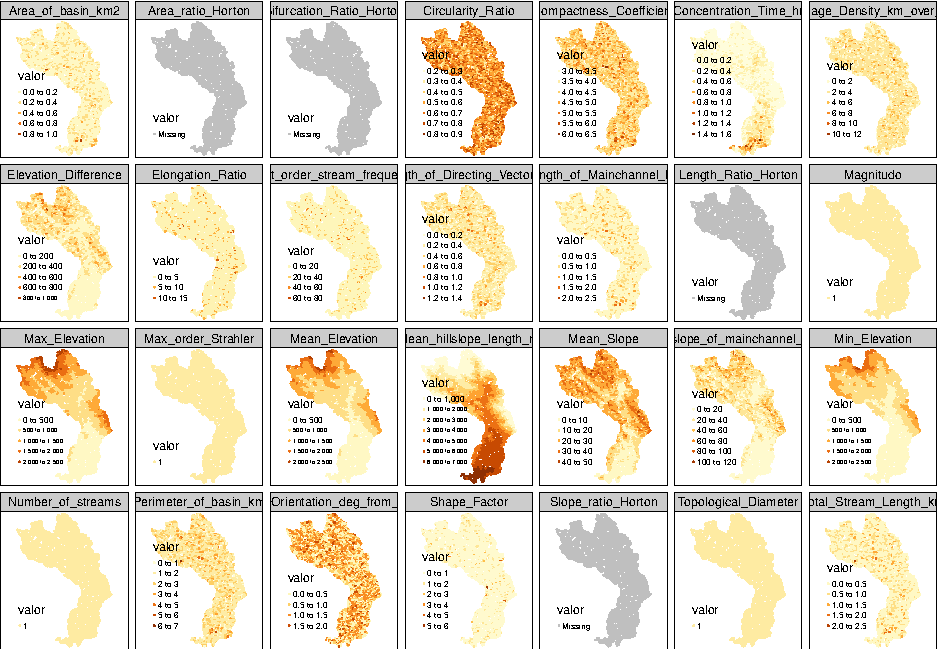
\includegraphics{proyecto_f_files/figure-latex/unnamed-chunk-62-1.pdf}

Tabla cols numéricas, con varianza

\begin{Shaded}
\begin{Highlighting}[]
\NormalTok{datosnum <-}\StringTok{ }\NormalTok{datos }\OperatorTok
\StringTok{  }\KeywordTok{st_drop_geometry}\NormalTok{() }\OperatorTok\StringTok{ }
\StringTok{  }\KeywordTok{select_if}\NormalTok{(is.numeric) }\OperatorTok\StringTok{ }
\StringTok{  }\KeywordTok{select_if}\NormalTok{(}\OperatorTok{~}\StringTok{ }\KeywordTok{sum}\NormalTok{(}\OperatorTok{!}\KeywordTok{is.na}\NormalTok{(.))}\OperatorTok{>}\DecValTok{0}\NormalTok{) }\OperatorTok\StringTok{ }
\StringTok{  }\KeywordTok{select_if}\NormalTok{(}\ControlFlowTok{function}\NormalTok{(x) }\KeywordTok{var}\NormalTok{(x, }\DataTypeTok{na.rm=}\NormalTok{T)}\OperatorTok{!=}\DecValTok{0}\NormalTok{)}
\end{Highlighting}
\end{Shaded}

Evaluación de correlación entre las variables como criterio de selección

\begin{Shaded}
\begin{Highlighting}[]
\NormalTok{datosnum }\OperatorTok\StringTok{ }\KeywordTok{ezCor}\NormalTok{(}\DataTypeTok{r_size_lims =} \DecValTok{2}\OperatorTok{:}\DecValTok{3}\NormalTok{, }\DataTypeTok{label_size =} \DecValTok{2}\NormalTok{)}
\end{Highlighting}
\end{Shaded}

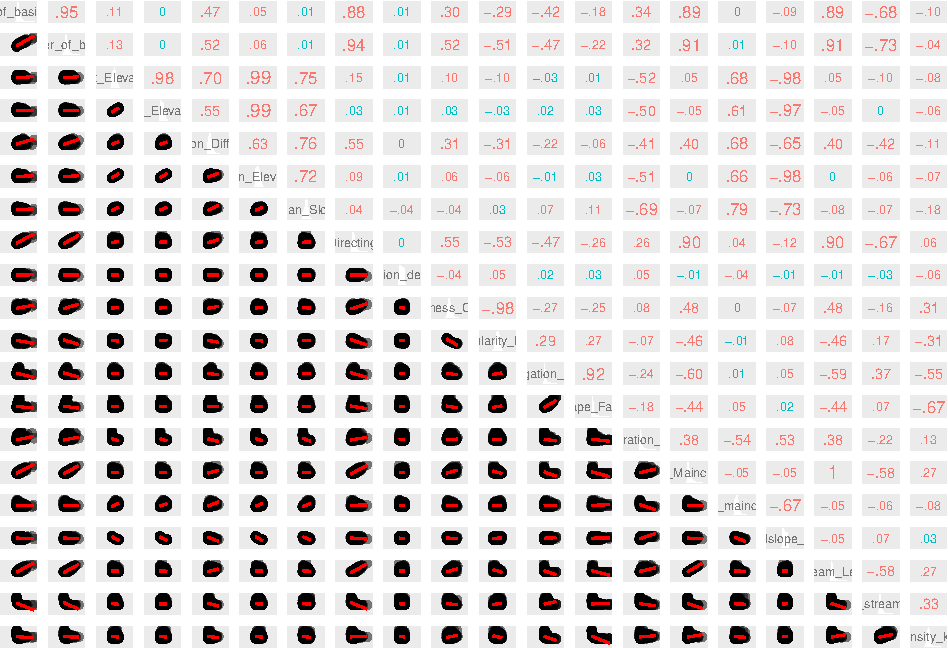
\includegraphics{proyecto_f_files/figure-latex/unnamed-chunk-64-1.pdf}

\begin{Shaded}
\begin{Highlighting}[]
\NormalTok{datosnum }\OperatorTok\StringTok{ }\NormalTok{cor}
\end{Highlighting}
\end{Shaded}

\begin{verbatim}
##                                          Area_of_basin_km2
## Area_of_basin_km2                             1.0000000000
## Perimeter_of_basin_km                         0.9544758340
## Max_Elevation                                 0.1085164535
## Min_Elevation                                -0.0037333059
## Elevation_Difference                          0.4687069509
## Mean_Elevation                                0.0527159463
## Mean_Slope                                    0.0116722827
## Length_of_Directing_Vector_km                 0.8821719458
## Prevalent_Orientation_deg_from_north_ccw      0.0133206854
## Compactness_Coefficient                       0.3026490133
## Circularity_Ratio                            -0.2885703636
## Elongation_Ratio                             -0.4201325677
## Shape_Factor                                 -0.1774118107
## Concentration_Time_hr                         0.3376141894
## Length_of_Mainchannel_km                      0.8868782573
## Mean_slope_of_mainchannel_percent            -0.0000623078
## Mean_hillslope_length_m                      -0.0868302019
## Total_Stream_Length_km                        0.8866554994
## First_order_stream_frequency                 -0.6765432843
## Drainage_Density_km_over_km2                 -0.0999198137
##                                          Perimeter_of_basin_km
## Area_of_basin_km2                                  0.954475834
## Perimeter_of_basin_km                              1.000000000
## Max_Elevation                                      0.126072976
## Min_Elevation                                      0.003374361
## Elevation_Difference                               0.517032317
## Mean_Elevation                                     0.064253895
## Mean_Slope                                         0.007432527
## Length_of_Directing_Vector_km                      0.941048386
## Prevalent_Orientation_deg_from_north_ccw           0.005013254
## Compactness_Coefficient                            0.524072883
## Circularity_Ratio                                 -0.505511388
## Elongation_Ratio                                  -0.465434321
## Shape_Factor                                      -0.222059361
## Concentration_Time_hr                              0.323183639
## Length_of_Mainchannel_km                           0.912566038
## Mean_slope_of_mainchannel_percent                  0.011612370
## Mean_hillslope_length_m                           -0.097546277
## Total_Stream_Length_km                             0.912065876
## First_order_stream_frequency                      -0.729729329
## Drainage_Density_km_over_km2                      -0.037858082
##                                          Max_Elevation Min_Elevation
## Area_of_basin_km2                          0.108516454  -0.003733306
## Perimeter_of_basin_km                      0.126072976   0.003374361
## Max_Elevation                              1.000000000   0.979845711
## Min_Elevation                              0.979845711   1.000000000
## Elevation_Difference                       0.701703589   0.545241433
## Mean_Elevation                             0.994679678   0.994064553
## Mean_Slope                                 0.750349000   0.669770309
## Length_of_Directing_Vector_km              0.152748940   0.026447839
## Prevalent_Orientation_deg_from_north_ccw   0.008534377   0.011223559
## Compactness_Coefficient                    0.097747484   0.026836115
## Circularity_Ratio                         -0.100979358  -0.030532368
## Elongation_Ratio                          -0.034917788   0.019213707
## Shape_Factor                               0.014803339   0.034733040
## Concentration_Time_hr                     -0.522952456  -0.499344963
## Length_of_Mainchannel_km                   0.050522470  -0.053047221
## Mean_slope_of_mainchannel_percent          0.682330464   0.612424193
## Mean_hillslope_length_m                   -0.976100493  -0.966412179
## Total_Stream_Length_km                     0.050305343  -0.053392624
## First_order_stream_frequency              -0.104632503  -0.004045040
## Drainage_Density_km_over_km2              -0.080209378  -0.063762484
##                                          Elevation_Difference
## Area_of_basin_km2                                 0.468706951
## Perimeter_of_basin_km                             0.517032317
## Max_Elevation                                     0.701703589
## Min_Elevation                                     0.545241433
## Elevation_Difference                              1.000000000
## Mean_Elevation                                    0.628662419
## Mean_Slope                                        0.759984277
## Length_of_Directing_Vector_km                     0.546682345
## Prevalent_Orientation_deg_from_north_ccw         -0.004216387
## Compactness_Coefficient                           0.314482816
## Circularity_Ratio                                -0.314862013
## Elongation_Ratio                                 -0.215062688
## Shape_Factor                                     -0.061759832
## Concentration_Time_hr                            -0.413566386
## Length_of_Mainchannel_km                          0.401222022
## Mean_slope_of_mainchannel_percent                 0.679079570
## Mean_hillslope_length_m                          -0.649322231
## Total_Stream_Length_km                            0.401542793
## First_order_stream_frequency                     -0.424664856
## Drainage_Density_km_over_km2                     -0.109178547
##                                          Mean_Elevation   Mean_Slope
## Area_of_basin_km2                           0.052715946  0.011672283
## Perimeter_of_basin_km                       0.064253895  0.007432527
## Max_Elevation                               0.994679678  0.750349000
## Min_Elevation                               0.994064553  0.669770309
## Elevation_Difference                        0.628662419  0.759984277
## Mean_Elevation                              1.000000000  0.717902080
## Mean_Slope                                  0.717902080  1.000000000
## Length_of_Directing_Vector_km               0.091595925  0.043152236
## Prevalent_Orientation_deg_from_north_ccw    0.008888368 -0.036953776
## Compactness_Coefficient                     0.058377050 -0.039121906
## Circularity_Ratio                          -0.061951571  0.031780506
## Elongation_Ratio                           -0.006958558  0.066886548
## Shape_Factor                                0.026491708  0.109470202
## Concentration_Time_hr                      -0.513112068 -0.688395113
## Length_of_Mainchannel_km                   -0.001812884 -0.074929355
## Mean_slope_of_mainchannel_percent           0.660296508  0.791702711
## Mean_hillslope_length_m                    -0.976432501 -0.725848165
## Total_Stream_Length_km                     -0.002122928 -0.075037094
## First_order_stream_frequency               -0.056487200 -0.070666731
## Drainage_Density_km_over_km2               -0.074394042 -0.178183177
##                                          Length_of_Directing_Vector_km
## Area_of_basin_km2                                           0.88217195
## Perimeter_of_basin_km                                       0.94104839
## Max_Elevation                                               0.15274894
## Min_Elevation                                               0.02644784
## Elevation_Difference                                        0.54668234
## Mean_Elevation                                              0.09159593
## Mean_Slope                                                  0.04315224
## Length_of_Directing_Vector_km                               1.00000000
## Prevalent_Orientation_deg_from_north_ccw                    0.00272695
## Compactness_Coefficient                                     0.54755642
## Circularity_Ratio                                          -0.53162055
## Elongation_Ratio                                           -0.47271463
## Shape_Factor                                               -0.26333595
## Concentration_Time_hr                                       0.26489121
## Length_of_Mainchannel_km                                    0.90154020
## Mean_slope_of_mainchannel_percent                           0.04130672
## Mean_hillslope_length_m                                    -0.12424888
## Total_Stream_Length_km                                      0.90087307
## First_order_stream_frequency                               -0.66625572
## Drainage_Density_km_over_km2                                0.05523891
##                                          Prevalent_Orientation_deg_from_north_ccw
## Area_of_basin_km2                                                     0.013320685
## Perimeter_of_basin_km                                                 0.005013254
## Max_Elevation                                                         0.008534377
## Min_Elevation                                                         0.011223559
## Elevation_Difference                                                 -0.004216387
## Mean_Elevation                                                        0.008888368
## Mean_Slope                                                           -0.036953776
## Length_of_Directing_Vector_km                                         0.002726950
## Prevalent_Orientation_deg_from_north_ccw                              1.000000000
## Compactness_Coefficient                                              -0.038263247
## Circularity_Ratio                                                     0.047959520
## Elongation_Ratio                                                      0.020435968
## Shape_Factor                                                          0.028979551
## Concentration_Time_hr                                                 0.045817442
## Length_of_Mainchannel_km                                             -0.014559540
## Mean_slope_of_mainchannel_percent                                    -0.041954144
## Mean_hillslope_length_m                                              -0.006101928
## Total_Stream_Length_km                                               -0.014834648
## First_order_stream_frequency                                         -0.025730089
## Drainage_Density_km_over_km2                                         -0.062373016
##                                          Compactness_Coefficient
## Area_of_basin_km2                                    0.302649013
## Perimeter_of_basin_km                                0.524072883
## Max_Elevation                                        0.097747484
## Min_Elevation                                        0.026836115
## Elevation_Difference                                 0.314482816
## Mean_Elevation                                       0.058377050
## Mean_Slope                                          -0.039121906
## Length_of_Directing_Vector_km                        0.547556416
## Prevalent_Orientation_deg_from_north_ccw            -0.038263247
## Compactness_Coefficient                              1.000000000
## Circularity_Ratio                                   -0.982893198
## Elongation_Ratio                                    -0.274815245
## Shape_Factor                                        -0.253076546
## Concentration_Time_hr                                0.084829477
## Length_of_Mainchannel_km                             0.477967483
## Mean_slope_of_mainchannel_percent                    0.002602623
## Mean_hillslope_length_m                             -0.074702534
## Total_Stream_Length_km                               0.476467186
## First_order_stream_frequency                        -0.161420996
## Drainage_Density_km_over_km2                         0.310395399
##                                          Circularity_Ratio
## Area_of_basin_km2                             -0.288570364
## Perimeter_of_basin_km                         -0.505511388
## Max_Elevation                                 -0.100979358
## Min_Elevation                                 -0.030532368
## Elevation_Difference                          -0.314862013
## Mean_Elevation                                -0.061951571
## Mean_Slope                                     0.031780506
## Length_of_Directing_Vector_km                 -0.531620546
## Prevalent_Orientation_deg_from_north_ccw       0.047959520
## Compactness_Coefficient                       -0.982893198
## Circularity_Ratio                              1.000000000
## Elongation_Ratio                               0.289513381
## Shape_Factor                                   0.265974071
## Concentration_Time_hr                         -0.074379454
## Length_of_Mainchannel_km                      -0.459171337
## Mean_slope_of_mainchannel_percent             -0.006744063
## Mean_hillslope_length_m                        0.078708721
## Total_Stream_Length_km                        -0.457493385
## First_order_stream_frequency                   0.168318540
## Drainage_Density_km_over_km2                  -0.309107811
##                                          Elongation_Ratio Shape_Factor
## Area_of_basin_km2                            -0.420132568  -0.17741181
## Perimeter_of_basin_km                        -0.465434321  -0.22205936
## Max_Elevation                                -0.034917788   0.01480334
## Min_Elevation                                 0.019213707   0.03473304
## Elevation_Difference                         -0.215062688  -0.06175983
## Mean_Elevation                               -0.006958558   0.02649171
## Mean_Slope                                    0.066886548   0.10947020
## Length_of_Directing_Vector_km                -0.472714634  -0.26333595
## Prevalent_Orientation_deg_from_north_ccw      0.020435968   0.02897955
## Compactness_Coefficient                      -0.274815245  -0.25307655
## Circularity_Ratio                             0.289513381   0.26597407
## Elongation_Ratio                              1.000000000   0.92166632
## Shape_Factor                                  0.921666316   1.00000000
## Concentration_Time_hr                        -0.244967627  -0.18437450
## Length_of_Mainchannel_km                     -0.595756838  -0.43862982
## Mean_slope_of_mainchannel_percent             0.013563039   0.05012741
## Mean_hillslope_length_m                       0.054309895   0.02193559
## Total_Stream_Length_km                       -0.594894045  -0.43777825
## First_order_stream_frequency                  0.370979755   0.06989293
## Drainage_Density_km_over_km2                 -0.546157778  -0.66918169
##                                          Concentration_Time_hr
## Area_of_basin_km2                                   0.33761419
## Perimeter_of_basin_km                               0.32318364
## Max_Elevation                                      -0.52295246
## Min_Elevation                                      -0.49934496
## Elevation_Difference                               -0.41356639
## Mean_Elevation                                     -0.51311207
## Mean_Slope                                         -0.68839511
## Length_of_Directing_Vector_km                       0.26489121
## Prevalent_Orientation_deg_from_north_ccw            0.04581744
## Compactness_Coefficient                             0.08482948
## Circularity_Ratio                                  -0.07437945
## Elongation_Ratio                                   -0.24496763
## Shape_Factor                                       -0.18437450
## Concentration_Time_hr                               1.00000000
## Length_of_Mainchannel_km                            0.37973458
## Mean_slope_of_mainchannel_percent                  -0.54157779
## Mean_hillslope_length_m                             0.53319066
## Total_Stream_Length_km                              0.37928755
## First_order_stream_frequency                       -0.22050640
## Drainage_Density_km_over_km2                        0.12574975
##                                          Length_of_Mainchannel_km
## Area_of_basin_km2                                     0.886878257
## Perimeter_of_basin_km                                 0.912566038
## Max_Elevation                                         0.050522470
## Min_Elevation                                        -0.053047221
## Elevation_Difference                                  0.401222022
## Mean_Elevation                                       -0.001812884
## Mean_Slope                                           -0.074929355
## Length_of_Directing_Vector_km                         0.901540197
## Prevalent_Orientation_deg_from_north_ccw             -0.014559540
## Compactness_Coefficient                               0.477967483
## Circularity_Ratio                                    -0.459171337
## Elongation_Ratio                                     -0.595756838
## Shape_Factor                                         -0.438629821
## Concentration_Time_hr                                 0.379734584
## Length_of_Mainchannel_km                              1.000000000
## Mean_slope_of_mainchannel_percent                    -0.048088478
## Mean_hillslope_length_m                              -0.053644883
## Total_Stream_Length_km                                0.999712141
## First_order_stream_frequency                         -0.577404672
## Drainage_Density_km_over_km2                          0.273665370
##                                          Mean_slope_of_mainchannel_percent
## Area_of_basin_km2                                            -0.0000623078
## Perimeter_of_basin_km                                         0.0116123695
## Max_Elevation                                                 0.6823304637
## Min_Elevation                                                 0.6124241933
## Elevation_Difference                                          0.6790795702
## Mean_Elevation                                                0.6602965081
## Mean_Slope                                                    0.7917027108
## Length_of_Directing_Vector_km                                 0.0413067240
## Prevalent_Orientation_deg_from_north_ccw                     -0.0419541444
## Compactness_Coefficient                                       0.0026026227
## Circularity_Ratio                                            -0.0067440632
## Elongation_Ratio                                              0.0135630387
## Shape_Factor                                                  0.0501274147
## Concentration_Time_hr                                        -0.5415777885
## Length_of_Mainchannel_km                                     -0.0480884780
## Mean_slope_of_mainchannel_percent                             1.0000000000
## Mean_hillslope_length_m                                      -0.6681192684
## Total_Stream_Length_km                                       -0.0474631511
## First_order_stream_frequency                                 -0.0557148988
## Drainage_Density_km_over_km2                                 -0.0801406065
##                                          Mean_hillslope_length_m
## Area_of_basin_km2                                   -0.086830202
## Perimeter_of_basin_km                               -0.097546277
## Max_Elevation                                       -0.976100493
## Min_Elevation                                       -0.966412179
## Elevation_Difference                                -0.649322231
## Mean_Elevation                                      -0.976432501
## Mean_Slope                                          -0.725848165
## Length_of_Directing_Vector_km                       -0.124248878
## Prevalent_Orientation_deg_from_north_ccw            -0.006101928
## Compactness_Coefficient                             -0.074702534
## Circularity_Ratio                                    0.078708721
## Elongation_Ratio                                     0.054309895
## Shape_Factor                                         0.021935590
## Concentration_Time_hr                                0.533190662
## Length_of_Mainchannel_km                            -0.053644883
## Mean_slope_of_mainchannel_percent                   -0.668119268
## Mean_hillslope_length_m                              1.000000000
## Total_Stream_Length_km                              -0.053467451
## First_order_stream_frequency                         0.068526699
## Drainage_Density_km_over_km2                         0.027552614
##                                          Total_Stream_Length_km
## Area_of_basin_km2                                   0.886655499
## Perimeter_of_basin_km                               0.912065876
## Max_Elevation                                       0.050305343
## Min_Elevation                                      -0.053392624
## Elevation_Difference                                0.401542793
## Mean_Elevation                                     -0.002122928
## Mean_Slope                                         -0.075037094
## Length_of_Directing_Vector_km                       0.900873075
## Prevalent_Orientation_deg_from_north_ccw           -0.014834648
## Compactness_Coefficient                             0.476467186
## Circularity_Ratio                                  -0.457493385
## Elongation_Ratio                                   -0.594894045
## Shape_Factor                                       -0.437778253
## Concentration_Time_hr                               0.379287551
## Length_of_Mainchannel_km                            0.999712141
## Mean_slope_of_mainchannel_percent                  -0.047463151
## Mean_hillslope_length_m                            -0.053467451
## Total_Stream_Length_km                              1.000000000
## First_order_stream_frequency                       -0.577169211
## Drainage_Density_km_over_km2                        0.274631240
##                                          First_order_stream_frequency
## Area_of_basin_km2                                         -0.67654328
## Perimeter_of_basin_km                                     -0.72972933
## Max_Elevation                                             -0.10463250
## Min_Elevation                                             -0.00404504
## Elevation_Difference                                      -0.42466486
## Mean_Elevation                                            -0.05648720
## Mean_Slope                                                -0.07066673
## Length_of_Directing_Vector_km                             -0.66625572
## Prevalent_Orientation_deg_from_north_ccw                  -0.02573009
## Compactness_Coefficient                                   -0.16142100
## Circularity_Ratio                                          0.16831854
## Elongation_Ratio                                           0.37097976
## Shape_Factor                                               0.06989293
## Concentration_Time_hr                                     -0.22050640
## Length_of_Mainchannel_km                                  -0.57740467
## Mean_slope_of_mainchannel_percent                         -0.05571490
## Mean_hillslope_length_m                                    0.06852670
## Total_Stream_Length_km                                    -0.57716921
## First_order_stream_frequency                               1.00000000
## Drainage_Density_km_over_km2                               0.33133675
##                                          Drainage_Density_km_over_km2
## Area_of_basin_km2                                         -0.09991981
## Perimeter_of_basin_km                                     -0.03785808
## Max_Elevation                                             -0.08020938
## Min_Elevation                                             -0.06376248
## Elevation_Difference                                      -0.10917855
## Mean_Elevation                                            -0.07439404
## Mean_Slope                                                -0.17818318
## Length_of_Directing_Vector_km                              0.05523891
## Prevalent_Orientation_deg_from_north_ccw                  -0.06237302
## Compactness_Coefficient                                    0.31039540
## Circularity_Ratio                                         -0.30910781
## Elongation_Ratio                                          -0.54615778
## Shape_Factor                                              -0.66918169
## Concentration_Time_hr                                      0.12574975
## Length_of_Mainchannel_km                                   0.27366537
## Mean_slope_of_mainchannel_percent                         -0.08014061
## Mean_hillslope_length_m                                    0.02755261
## Total_Stream_Length_km                                     0.27463124
## First_order_stream_frequency                               0.33133675
## Drainage_Density_km_over_km2                               1.00000000
\end{verbatim}

Union espacial de las variables seleccionadas

\begin{Shaded}
\begin{Highlighting}[]
\NormalTok{VARSEL <-}\StringTok{ }\NormalTok{datos }\OperatorTok\StringTok{ }
\StringTok{  }\NormalTok{dplyr}\OperatorTok{::}\KeywordTok{select}\NormalTok{(}
    \DataTypeTok{DD =}\NormalTok{ Drainage_Density_km_over_km2,}
    \DataTypeTok{SF =}\NormalTok{ Shape_Factor,}
    \DataTypeTok{ER =}\NormalTok{ Elongation_Ratio,}
    \DataTypeTok{TS =}\NormalTok{ Total_Stream_Length_km,}
    \DataTypeTok{MS =}\NormalTok{ Mean_Slope}
\NormalTok{  )}

\NormalTok{Varselpol1 <-}\StringTok{ }\NormalTok{pol1 }\OperatorTok\StringTok{ }\KeywordTok{st_join}\NormalTok{(}\DataTypeTok{left =}\NormalTok{ F, VARSEL)}
\NormalTok{Varselpol2 <-}\StringTok{ }\NormalTok{Varselpol1 }\OperatorTok\StringTok{ }
\StringTok{  }\KeywordTok{mutate}\NormalTok{(}\DataTypeTok{logDD =} \KeywordTok{log}\NormalTok{(DD))}
\end{Highlighting}
\end{Shaded}

Creación de objeto XY con atributos del objeto Varselpol2 mediante el
centroide de los polígonos

\begin{Shaded}
\begin{Highlighting}[]
\NormalTok{xy <-}\StringTok{ }\NormalTok{Varselpol2 }\OperatorTok
\StringTok{  }\KeywordTok{st_centroid}\NormalTok{() }\OperatorTok\StringTok{ }
\StringTok{  }\KeywordTok{mutate}\NormalTok{(}\DataTypeTok{x=}\KeywordTok{unlist}\NormalTok{(}\KeywordTok{map}\NormalTok{(geometry,}\DecValTok{1}\NormalTok{)),}
         \DataTypeTok{y=}\KeywordTok{unlist}\NormalTok{(}\KeywordTok{map}\NormalTok{(geometry,}\DecValTok{2}\NormalTok{))) }\OperatorTok\StringTok{ }
\StringTok{  }\KeywordTok{st_drop_geometry}\NormalTok{() }\OperatorTok\StringTok{ }
\StringTok{  }\KeywordTok{select}\NormalTok{(fid, x, y)}
\end{Highlighting}
\end{Shaded}

Creación del objeto Varselpol3 mediante unión de XY y Varselpol2

\begin{Shaded}
\begin{Highlighting}[]
\NormalTok{Varselpol3 <-}\StringTok{ }\NormalTok{Varselpol2 }\OperatorTok\StringTok{ }
\StringTok{  }\KeywordTok{inner_join}\NormalTok{(xy)}
\NormalTok{Varselpol3}
\end{Highlighting}
\end{Shaded}

\begin{verbatim}
## Simple feature collection with 3027 features and 12 fields
## geometry type:  POLYGON
## dimension:      XY
## bbox:           xmin: 317400 ymin: 2019180 xmax: 352260 ymax: 2067690
## epsg (SRID):    32619
## proj4string:    +proj=utm +zone=19 +datum=WGS84 +units=m +no_defs
## First 10 features:
##        fid cat value label       DD        SF        ER     TS    MS
## 1  3.0e+09   2     1       2.189137 0.4974215 1.1522986 0.5194 26.44
## 2  4.0e+09   3     3       1.317045 1.5193957 6.7526210 0.0849 31.26
## 3  5.0e+09   7     2       5.021898 0.2158705 0.8774590 0.3870 24.12
## 4  6.0e+09  11    18       3.348350 0.3116489 0.7588246 0.7191 27.12
## 5  7.0e+09   8     8       1.323741 0.9530676 3.2504695 0.1449 36.98
## 6  8.0e+09   9     4       5.407681 0.2022916 0.7547642 0.4946 23.41
## 7  9.0e+09  12    10       1.707515 0.6384885 1.5645024 0.3621 34.67
## 8  1.0e+10  14     9       1.776552 0.7101480 2.8058127 0.1449 37.30
## 9  1.1e+10  15    14       1.017378 1.2400654 3.7077166 0.1449 37.36
## 10 1.2e+10  10    13       1.376470 0.8268738 2.2012308 0.2473 30.57
##        logDD        x       y                       geometry
## 1  0.7835072 334063.9 2067449 POLYGON ((334500 2067660, 3...
## 2  0.2753904 334582.9 2067514 POLYGON ((334500 2067390, 3...
## 3  1.6138079 334172.4 2067265 POLYGON ((334440 2067330, 3...
## 4  1.2084677 334366.4 2066754 POLYGON ((333840 2067180, 3...
## 5  0.2804618 333919.7 2066981 POLYGON ((333750 2067240, 3...
## 6  1.6878203 334365.9 2067039 POLYGON ((334380 2067240, 3...
## 7  0.5350394 333028.9 2066963 POLYGON ((332640 2067120, 3...
## 8  0.5746743 333771.9 2066901 POLYGON ((333540 2067090, 3...
## 9  0.0172283 333384.3 2066840 POLYGON ((333330 2067090, 3...
## 10 0.3195221 332580.6 2066931 POLYGON ((332280 2067000, 3...
\end{verbatim}

\textbf{VECINDAD. Análisis de vecindad por contiguidad}

\begin{Shaded}
\begin{Highlighting}[]
\NormalTok{Varselpol3 <-}\StringTok{ }\NormalTok{Varselpol2 }\OperatorTok\StringTok{ }
\StringTok{  }\KeywordTok{inner_join}\NormalTok{(xy)}
\end{Highlighting}
\end{Shaded}

\begin{verbatim}
## Joining, by = "fid"
\end{verbatim}

\begin{Shaded}
\begin{Highlighting}[]
\NormalTok{Varselpol3}
\end{Highlighting}
\end{Shaded}

\begin{verbatim}
## Simple feature collection with 3027 features and 12 fields
## geometry type:  POLYGON
## dimension:      XY
## bbox:           xmin: 317400 ymin: 2019180 xmax: 352260 ymax: 2067690
## epsg (SRID):    32619
## proj4string:    +proj=utm +zone=19 +datum=WGS84 +units=m +no_defs
## First 10 features:
##        fid cat value label       DD        SF        ER     TS    MS
## 1  3.0e+09   2     1       2.189137 0.4974215 1.1522986 0.5194 26.44
## 2  4.0e+09   3     3       1.317045 1.5193957 6.7526210 0.0849 31.26
## 3  5.0e+09   7     2       5.021898 0.2158705 0.8774590 0.3870 24.12
## 4  6.0e+09  11    18       3.348350 0.3116489 0.7588246 0.7191 27.12
## 5  7.0e+09   8     8       1.323741 0.9530676 3.2504695 0.1449 36.98
## 6  8.0e+09   9     4       5.407681 0.2022916 0.7547642 0.4946 23.41
## 7  9.0e+09  12    10       1.707515 0.6384885 1.5645024 0.3621 34.67
## 8  1.0e+10  14     9       1.776552 0.7101480 2.8058127 0.1449 37.30
## 9  1.1e+10  15    14       1.017378 1.2400654 3.7077166 0.1449 37.36
## 10 1.2e+10  10    13       1.376470 0.8268738 2.2012308 0.2473 30.57
##        logDD        x       y                       geometry
## 1  0.7835072 334063.9 2067449 POLYGON ((334500 2067660, 3...
## 2  0.2753904 334582.9 2067514 POLYGON ((334500 2067390, 3...
## 3  1.6138079 334172.4 2067265 POLYGON ((334440 2067330, 3...
## 4  1.2084677 334366.4 2066754 POLYGON ((333840 2067180, 3...
## 5  0.2804618 333919.7 2066981 POLYGON ((333750 2067240, 3...
## 6  1.6878203 334365.9 2067039 POLYGON ((334380 2067240, 3...
## 7  0.5350394 333028.9 2066963 POLYGON ((332640 2067120, 3...
## 8  0.5746743 333771.9 2066901 POLYGON ((333540 2067090, 3...
## 9  0.0172283 333384.3 2066840 POLYGON ((333330 2067090, 3...
## 10 0.3195221 332580.6 2066931 POLYGON ((332280 2067000, 3...
\end{verbatim}

Análisis de Vecindad por cantidad de los 5 vecinos más cercanos

\begin{Shaded}
\begin{Highlighting}[]
\NormalTok{Varselpol3.sp <-}\StringTok{ }\KeywordTok{as_Spatial}\NormalTok{(Varselpol3)}
\NormalTok{coords <-}\StringTok{ }\KeywordTok{coordinates}\NormalTok{(Varselpol3.sp)}
\NormalTok{VecxK <-}\StringTok{ }\KeywordTok{knn2nb}\NormalTok{(}\KeywordTok{knearneigh}\NormalTok{(coords, }\DataTypeTok{k=}\DecValTok{5}\NormalTok{))}
\end{Highlighting}
\end{Shaded}

Análisis de Vecindad por peso de observaciones vecinas en Varselpol3

\begin{Shaded}
\begin{Highlighting}[]
\NormalTok{PesoW <-}\StringTok{ }\KeywordTok{nb2listw}\NormalTok{(VecxK)}
\NormalTok{PesoW}
\end{Highlighting}
\end{Shaded}

\begin{verbatim}
## Characteristics of weights list object:
## Neighbour list object:
## Number of regions: 3027 
## Number of nonzero links: 15135 
## Percentage nonzero weights: 0.16518 
## Average number of links: 5 
## Non-symmetric neighbours list
## 
## Weights style: W 
## Weights constants summary:
##      n      nn   S0      S1       S2
## W 3027 9162729 3027 1111.88 12356.64
\end{verbatim}

\begin{Shaded}
\begin{Highlighting}[]
\NormalTok{PesowB <-}\StringTok{ }\KeywordTok{nb2listw}\NormalTok{(VecxK, }\DataTypeTok{style =} \StringTok{'B'}\NormalTok{)}
\NormalTok{PesowB}
\end{Highlighting}
\end{Shaded}

\begin{verbatim}
## Characteristics of weights list object:
## Neighbour list object:
## Number of regions: 3027 
## Number of nonzero links: 15135 
## Percentage nonzero weights: 0.16518 
## Average number of links: 5 
## Non-symmetric neighbours list
## 
## Weights style: B 
## Weights constants summary:
##      n      nn    S0    S1     S2
## B 3027 9162729 15135 27797 308916
\end{verbatim}

Análisis de Vecindad por peso de observaciones vecinas en la data
completa

\begin{Shaded}
\begin{Highlighting}[]
\NormalTok{datos <-}\StringTok{ }\NormalTok{datos }\OperatorTok\StringTok{ }\KeywordTok{st_difference}\NormalTok{()}
\NormalTok{coords <-}\StringTok{ }\KeywordTok{coordinates}\NormalTok{(}\KeywordTok{as_Spatial}\NormalTok{(datos))}
\NormalTok{nb <-}\StringTok{ }\KeywordTok{knn2nb}\NormalTok{(}\KeywordTok{knearneigh}\NormalTok{(coords, }\DataTypeTok{k =} \DecValTok{5}\NormalTok{))}
\KeywordTok{summary}\NormalTok{(nb)}
\end{Highlighting}
\end{Shaded}

\begin{verbatim}
## Neighbour list object:
## Number of regions: 3027 
## Number of nonzero links: 15135 
## Percentage nonzero weights: 0.16518 
## Average number of links: 5 
## Non-symmetric neighbours list
## Link number distribution:
## 
##    5 
## 3027 
## 3027 least connected regions:
## 1 2 3 4 5 6 7 8 9 10 11 12 13 14 15 16 17 18 19 20 21 22 23 24 25 26 27 28 29 30 31 32 33 34 35 36 37 38 39 40 41 42 43 44 45 46 47 48 49 50 51 52 53 54 55 56 57 58 59 60 61 62 63 64 65 66 67 68 69 70 71 72 73 74 75 76 77 78 79 80 81 82 83 84 85 86 87 88 89 90 91 92 93 94 95 96 97 98 99 100 101 102 103 104 105 106 107 108 109 110 111 112 113 114 115 116 117 118 119 120 121 122 123 124 125 126 127 128 129 130 131 132 133 134 135 136 137 138 139 140 141 142 143 144 145 146 147 148 149 150 151 152 153 154 155 156 157 158 159 160 161 162 163 164 165 166 167 168 169 170 171 172 173 174 175 176 177 178 179 180 181 182 183 184 185 186 187 188 189 190 191 192 193 194 195 196 197 198 199 200 201 202 203 204 205 206 207 208 209 210 211 212 213 214 215 216 217 218 219 220 221 222 223 224 225 226 227 228 229 230 231 232 233 234 235 236 237 238 239 240 241 242 243 244 245 246 247 248 249 250 251 252 253 254 255 256 257 258 259 260 261 262 263 264 265 266 267 268 269 270 271 272 273 274 275 276 277 278 279 280 281 282 283 284 285 286 287 288 289 290 291 292 293 294 295 296 297 298 299 300 301 302 303 304 305 306 307 308 309 310 311 312 313 314 315 316 317 318 319 320 321 322 323 324 325 326 327 328 329 330 331 332 333 334 335 336 337 338 339 340 341 342 343 344 345 346 347 348 349 350 351 352 353 354 355 356 357 358 359 360 361 362 363 364 365 366 367 368 369 370 371 372 373 374 375 376 377 378 379 380 381 382 383 384 385 386 387 388 389 390 391 392 393 394 395 396 397 398 399 400 401 402 403 404 405 406 407 408 409 410 411 412 413 414 415 416 417 418 419 420 421 422 423 424 425 426 427 428 429 430 431 432 433 434 435 436 437 438 439 440 441 442 443 444 445 446 447 448 449 450 451 452 453 454 455 456 457 458 459 460 461 462 463 464 465 466 467 468 469 470 471 472 473 474 475 476 477 478 479 480 481 482 483 484 485 486 487 488 489 490 491 492 493 494 495 496 497 498 499 500 501 502 503 504 505 506 507 508 509 510 511 512 513 514 515 516 517 518 519 520 521 522 523 524 525 526 527 528 529 530 531 532 533 534 535 536 537 538 539 540 541 542 543 544 545 546 547 548 549 550 551 552 553 554 555 556 557 558 559 560 561 562 563 564 565 566 567 568 569 570 571 572 573 574 575 576 577 578 579 580 581 582 583 584 585 586 587 588 589 590 591 592 593 594 595 596 597 598 599 600 601 602 603 604 605 606 607 608 609 610 611 612 613 614 615 616 617 618 619 620 621 622 623 624 625 626 627 628 629 630 631 632 633 634 635 636 637 638 639 640 641 642 643 644 645 646 647 648 649 650 651 652 653 654 655 656 657 658 659 660 661 662 663 664 665 666 667 668 669 670 671 672 673 674 675 676 677 678 679 680 681 682 683 684 685 686 687 688 689 690 691 692 693 694 695 696 697 698 699 700 701 702 703 704 705 706 707 708 709 710 711 712 713 714 715 716 717 718 719 720 721 722 723 724 725 726 727 728 729 730 731 732 733 734 735 736 737 738 739 740 741 742 743 744 745 746 747 748 749 750 751 752 753 754 755 756 757 758 759 760 761 762 763 764 765 766 767 768 769 770 771 772 773 774 775 776 777 778 779 780 781 782 783 784 785 786 787 788 789 790 791 792 793 794 795 796 797 798 799 800 801 802 803 804 805 806 807 808 809 810 811 812 813 814 815 816 817 818 819 820 821 822 823 824 825 826 827 828 829 830 831 832 833 834 835 836 837 838 839 840 841 842 843 844 845 846 847 848 849 850 851 852 853 854 855 856 857 858 859 860 861 862 863 864 865 866 867 868 869 870 871 872 873 874 875 876 877 878 879 880 881 882 883 884 885 886 887 888 889 890 891 892 893 894 895 896 897 898 899 900 901 902 903 904 905 906 907 908 909 910 911 912 913 914 915 916 917 918 919 920 921 922 923 924 925 926 927 928 929 930 931 932 933 934 935 936 937 938 939 940 941 942 943 944 945 946 947 948 949 950 951 952 953 954 955 956 957 958 959 960 961 962 963 964 965 966 967 968 969 970 971 972 973 974 975 976 977 978 979 980 981 982 983 984 985 986 987 988 989 990 991 992 993 994 995 996 997 998 999 1000 1001 1002 1003 1004 1005 1006 1007 1008 1009 1010 1011 1012 1013 1014 1015 1016 1017 1018 1019 1020 1021 1022 1023 1024 1025 1026 1027 1028 1029 1030 1031 1032 1033 1034 1035 1036 1037 1038 1039 1040 1041 1042 1043 1044 1045 1046 1047 1048 1049 1050 1051 1052 1053 1054 1055 1056 1057 1058 1059 1060 1061 1062 1063 1064 1065 1066 1067 1068 1069 1070 1071 1072 1073 1074 1075 1076 1077 1078 1079 1080 1081 1082 1083 1084 1085 1086 1087 1088 1089 1090 1091 1092 1093 1094 1095 1096 1097 1098 1099 1100 1101 1102 1103 1104 1105 1106 1107 1108 1109 1110 1111 1112 1113 1114 1115 1116 1117 1118 1119 1120 1121 1122 1123 1124 1125 1126 1127 1128 1129 1130 1131 1132 1133 1134 1135 1136 1137 1138 1139 1140 1141 1142 1143 1144 1145 1146 1147 1148 1149 1150 1151 1152 1153 1154 1155 1156 1157 1158 1159 1160 1161 1162 1163 1164 1165 1166 1167 1168 1169 1170 1171 1172 1173 1174 1175 1176 1177 1178 1179 1180 1181 1182 1183 1184 1185 1186 1187 1188 1189 1190 1191 1192 1193 1194 1195 1196 1197 1198 1199 1200 1201 1202 1203 1204 1205 1206 1207 1208 1209 1210 1211 1212 1213 1214 1215 1216 1217 1218 1219 1220 1221 1222 1223 1224 1225 1226 1227 1228 1229 1230 1231 1232 1233 1234 1235 1236 1237 1238 1239 1240 1241 1242 1243 1244 1245 1246 1247 1248 1249 1250 1251 1252 1253 1254 1255 1256 1257 1258 1259 1260 1261 1262 1263 1264 1265 1266 1267 1268 1269 1270 1271 1272 1273 1274 1275 1276 1277 1278 1279 1280 1281 1282 1283 1284 1285 1286 1287 1288 1289 1290 1291 1292 1293 1294 1295 1296 1297 1298 1299 1300 1301 1302 1303 1304 1305 1306 1307 1308 1309 1310 1311 1312 1313 1314 1315 1316 1317 1318 1319 1320 1321 1322 1323 1324 1325 1326 1327 1328 1329 1330 1331 1332 1333 1334 1335 1336 1337 1338 1339 1340 1341 1342 1343 1344 1345 1346 1347 1348 1349 1350 1351 1352 1353 1354 1355 1356 1357 1358 1359 1360 1361 1362 1363 1364 1365 1366 1367 1368 1369 1370 1371 1372 1373 1374 1375 1376 1377 1378 1379 1380 1381 1382 1383 1384 1385 1386 1387 1388 1389 1390 1391 1392 1393 1394 1395 1396 1397 1398 1399 1400 1401 1402 1403 1404 1405 1406 1407 1408 1409 1410 1411 1412 1413 1414 1415 1416 1417 1418 1419 1420 1421 1422 1423 1424 1425 1426 1427 1428 1429 1430 1431 1432 1433 1434 1435 1436 1437 1438 1439 1440 1441 1442 1443 1444 1445 1446 1447 1448 1449 1450 1451 1452 1453 1454 1455 1456 1457 1458 1459 1460 1461 1462 1463 1464 1465 1466 1467 1468 1469 1470 1471 1472 1473 1474 1475 1476 1477 1478 1479 1480 1481 1482 1483 1484 1485 1486 1487 1488 1489 1490 1491 1492 1493 1494 1495 1496 1497 1498 1499 1500 1501 1502 1503 1504 1505 1506 1507 1508 1509 1510 1511 1512 1513 1514 1515 1516 1517 1518 1519 1520 1521 1522 1523 1524 1525 1526 1527 1528 1529 1530 1531 1532 1533 1534 1535 1536 1537 1538 1539 1540 1541 1542 1543 1544 1545 1546 1547 1548 1549 1550 1551 1552 1553 1554 1555 1556 1557 1558 1559 1560 1561 1562 1563 1564 1565 1566 1567 1568 1569 1570 1571 1572 1573 1574 1575 1576 1577 1578 1579 1580 1581 1582 1583 1584 1585 1586 1587 1588 1589 1590 1591 1592 1593 1594 1595 1596 1597 1598 1599 1600 1601 1602 1603 1604 1605 1606 1607 1608 1609 1610 1611 1612 1613 1614 1615 1616 1617 1618 1619 1620 1621 1622 1623 1624 1625 1626 1627 1628 1629 1630 1631 1632 1633 1634 1635 1636 1637 1638 1639 1640 1641 1642 1643 1644 1645 1646 1647 1648 1649 1650 1651 1652 1653 1654 1655 1656 1657 1658 1659 1660 1661 1662 1663 1664 1665 1666 1667 1668 1669 1670 1671 1672 1673 1674 1675 1676 1677 1678 1679 1680 1681 1682 1683 1684 1685 1686 1687 1688 1689 1690 1691 1692 1693 1694 1695 1696 1697 1698 1699 1700 1701 1702 1703 1704 1705 1706 1707 1708 1709 1710 1711 1712 1713 1714 1715 1716 1717 1718 1719 1720 1721 1722 1723 1724 1725 1726 1727 1728 1729 1730 1731 1732 1733 1734 1735 1736 1737 1738 1739 1740 1741 1742 1743 1744 1745 1746 1747 1748 1749 1750 1751 1752 1753 1754 1755 1756 1757 1758 1759 1760 1761 1762 1763 1764 1765 1766 1767 1768 1769 1770 1771 1772 1773 1774 1775 1776 1777 1778 1779 1780 1781 1782 1783 1784 1785 1786 1787 1788 1789 1790 1791 1792 1793 1794 1795 1796 1797 1798 1799 1800 1801 1802 1803 1804 1805 1806 1807 1808 1809 1810 1811 1812 1813 1814 1815 1816 1817 1818 1819 1820 1821 1822 1823 1824 1825 1826 1827 1828 1829 1830 1831 1832 1833 1834 1835 1836 1837 1838 1839 1840 1841 1842 1843 1844 1845 1846 1847 1848 1849 1850 1851 1852 1853 1854 1855 1856 1857 1858 1859 1860 1861 1862 1863 1864 1865 1866 1867 1868 1869 1870 1871 1872 1873 1874 1875 1876 1877 1878 1879 1880 1881 1882 1883 1884 1885 1886 1887 1888 1889 1890 1891 1892 1893 1894 1895 1896 1897 1898 1899 1900 1901 1902 1903 1904 1905 1906 1907 1908 1909 1910 1911 1912 1913 1914 1915 1916 1917 1918 1919 1920 1921 1922 1923 1924 1925 1926 1927 1928 1929 1930 1931 1932 1933 1934 1935 1936 1937 1938 1939 1940 1941 1942 1943 1944 1945 1946 1947 1948 1949 1950 1951 1952 1953 1954 1955 1956 1957 1958 1959 1960 1961 1962 1963 1964 1965 1966 1967 1968 1969 1970 1971 1972 1973 1974 1975 1976 1977 1978 1979 1980 1981 1982 1983 1984 1985 1986 1987 1988 1989 1990 1991 1992 1993 1994 1995 1996 1997 1998 1999 2000 2001 2002 2003 2004 2005 2006 2007 2008 2009 2010 2011 2012 2013 2014 2015 2016 2017 2018 2019 2020 2021 2022 2023 2024 2025 2026 2027 2028 2029 2030 2031 2032 2033 2034 2035 2036 2037 2038 2039 2040 2041 2042 2043 2044 2045 2046 2047 2048 2049 2050 2051 2052 2053 2054 2055 2056 2057 2058 2059 2060 2061 2062 2063 2064 2065 2066 2067 2068 2069 2070 2071 2072 2073 2074 2075 2076 2077 2078 2079 2080 2081 2082 2083 2084 2085 2086 2087 2088 2089 2090 2091 2092 2093 2094 2095 2096 2097 2098 2099 2100 2101 2102 2103 2104 2105 2106 2107 2108 2109 2110 2111 2112 2113 2114 2115 2116 2117 2118 2119 2120 2121 2122 2123 2124 2125 2126 2127 2128 2129 2130 2131 2132 2133 2134 2135 2136 2137 2138 2139 2140 2141 2142 2143 2144 2145 2146 2147 2148 2149 2150 2151 2152 2153 2154 2155 2156 2157 2158 2159 2160 2161 2162 2163 2164 2165 2166 2167 2168 2169 2170 2171 2172 2173 2174 2175 2176 2177 2178 2179 2180 2181 2182 2183 2184 2185 2186 2187 2188 2189 2190 2191 2192 2193 2194 2195 2196 2197 2198 2199 2200 2201 2202 2203 2204 2205 2206 2207 2208 2209 2210 2211 2212 2213 2214 2215 2216 2217 2218 2219 2220 2221 2222 2223 2224 2225 2226 2227 2228 2229 2230 2231 2232 2233 2234 2235 2236 2237 2238 2239 2240 2241 2242 2243 2244 2245 2246 2247 2248 2249 2250 2251 2252 2253 2254 2255 2256 2257 2258 2259 2260 2261 2262 2263 2264 2265 2266 2267 2268 2269 2270 2271 2272 2273 2274 2275 2276 2277 2278 2279 2280 2281 2282 2283 2284 2285 2286 2287 2288 2289 2290 2291 2292 2293 2294 2295 2296 2297 2298 2299 2300 2301 2302 2303 2304 2305 2306 2307 2308 2309 2310 2311 2312 2313 2314 2315 2316 2317 2318 2319 2320 2321 2322 2323 2324 2325 2326 2327 2328 2329 2330 2331 2332 2333 2334 2335 2336 2337 2338 2339 2340 2341 2342 2343 2344 2345 2346 2347 2348 2349 2350 2351 2352 2353 2354 2355 2356 2357 2358 2359 2360 2361 2362 2363 2364 2365 2366 2367 2368 2369 2370 2371 2372 2373 2374 2375 2376 2377 2378 2379 2380 2381 2382 2383 2384 2385 2386 2387 2388 2389 2390 2391 2392 2393 2394 2395 2396 2397 2398 2399 2400 2401 2402 2403 2404 2405 2406 2407 2408 2409 2410 2411 2412 2413 2414 2415 2416 2417 2418 2419 2420 2421 2422 2423 2424 2425 2426 2427 2428 2429 2430 2431 2432 2433 2434 2435 2436 2437 2438 2439 2440 2441 2442 2443 2444 2445 2446 2447 2448 2449 2450 2451 2452 2453 2454 2455 2456 2457 2458 2459 2460 2461 2462 2463 2464 2465 2466 2467 2468 2469 2470 2471 2472 2473 2474 2475 2476 2477 2478 2479 2480 2481 2482 2483 2484 2485 2486 2487 2488 2489 2490 2491 2492 2493 2494 2495 2496 2497 2498 2499 2500 2501 2502 2503 2504 2505 2506 2507 2508 2509 2510 2511 2512 2513 2514 2515 2516 2517 2518 2519 2520 2521 2522 2523 2524 2525 2526 2527 2528 2529 2530 2531 2532 2533 2534 2535 2536 2537 2538 2539 2540 2541 2542 2543 2544 2545 2546 2547 2548 2549 2550 2551 2552 2553 2554 2555 2556 2557 2558 2559 2560 2561 2562 2563 2564 2565 2566 2567 2568 2569 2570 2571 2572 2573 2574 2575 2576 2577 2578 2579 2580 2581 2582 2583 2584 2585 2586 2587 2588 2589 2590 2591 2592 2593 2594 2595 2596 2597 2598 2599 2600 2601 2602 2603 2604 2605 2606 2607 2608 2609 2610 2611 2612 2613 2614 2615 2616 2617 2618 2619 2620 2621 2622 2623 2624 2625 2626 2627 2628 2629 2630 2631 2632 2633 2634 2635 2636 2637 2638 2639 2640 2641 2642 2643 2644 2645 2646 2647 2648 2649 2650 2651 2652 2653 2654 2655 2656 2657 2658 2659 2660 2661 2662 2663 2664 2665 2666 2667 2668 2669 2670 2671 2672 2673 2674 2675 2676 2677 2678 2679 2680 2681 2682 2683 2684 2685 2686 2687 2688 2689 2690 2691 2692 2693 2694 2695 2696 2697 2698 2699 2700 2701 2702 2703 2704 2705 2706 2707 2708 2709 2710 2711 2712 2713 2714 2715 2716 2717 2718 2719 2720 2721 2722 2723 2724 2725 2726 2727 2728 2729 2730 2731 2732 2733 2734 2735 2736 2737 2738 2739 2740 2741 2742 2743 2744 2745 2746 2747 2748 2749 2750 2751 2752 2753 2754 2755 2756 2757 2758 2759 2760 2761 2762 2763 2764 2765 2766 2767 2768 2769 2770 2771 2772 2773 2774 2775 2776 2777 2778 2779 2780 2781 2782 2783 2784 2785 2786 2787 2788 2789 2790 2791 2792 2793 2794 2795 2796 2797 2798 2799 2800 2801 2802 2803 2804 2805 2806 2807 2808 2809 2810 2811 2812 2813 2814 2815 2816 2817 2818 2819 2820 2821 2822 2823 2824 2825 2826 2827 2828 2829 2830 2831 2832 2833 2834 2835 2836 2837 2838 2839 2840 2841 2842 2843 2844 2845 2846 2847 2848 2849 2850 2851 2852 2853 2854 2855 2856 2857 2858 2859 2860 2861 2862 2863 2864 2865 2866 2867 2868 2869 2870 2871 2872 2873 2874 2875 2876 2877 2878 2879 2880 2881 2882 2883 2884 2885 2886 2887 2888 2889 2890 2891 2892 2893 2894 2895 2896 2897 2898 2899 2900 2901 2902 2903 2904 2905 2906 2907 2908 2909 2910 2911 2912 2913 2914 2915 2916 2917 2918 2919 2920 2921 2922 2923 2924 2925 2926 2927 2928 2929 2930 2931 2932 2933 2934 2935 2936 2937 2938 2939 2940 2941 2942 2943 2944 2945 2946 2947 2948 2949 2950 2951 2952 2953 2954 2955 2956 2957 2958 2959 2960 2961 2962 2963 2964 2965 2966 2967 2968 2969 2970 2971 2972 2973 2974 2975 2976 2977 2978 2979 2980 2981 2982 2983 2984 2985 2986 2987 2988 2989 2990 2991 2992 2993 2994 2995 2996 2997 2998 2999 3000 3001 3002 3003 3004 3005 3006 3007 3008 3009 3010 3011 3012 3013 3014 3015 3016 3017 3018 3019 3020 3021 3022 3023 3024 3025 3026 3027 with 5 links
## 3027 most connected regions:
## 1 2 3 4 5 6 7 8 9 10 11 12 13 14 15 16 17 18 19 20 21 22 23 24 25 26 27 28 29 30 31 32 33 34 35 36 37 38 39 40 41 42 43 44 45 46 47 48 49 50 51 52 53 54 55 56 57 58 59 60 61 62 63 64 65 66 67 68 69 70 71 72 73 74 75 76 77 78 79 80 81 82 83 84 85 86 87 88 89 90 91 92 93 94 95 96 97 98 99 100 101 102 103 104 105 106 107 108 109 110 111 112 113 114 115 116 117 118 119 120 121 122 123 124 125 126 127 128 129 130 131 132 133 134 135 136 137 138 139 140 141 142 143 144 145 146 147 148 149 150 151 152 153 154 155 156 157 158 159 160 161 162 163 164 165 166 167 168 169 170 171 172 173 174 175 176 177 178 179 180 181 182 183 184 185 186 187 188 189 190 191 192 193 194 195 196 197 198 199 200 201 202 203 204 205 206 207 208 209 210 211 212 213 214 215 216 217 218 219 220 221 222 223 224 225 226 227 228 229 230 231 232 233 234 235 236 237 238 239 240 241 242 243 244 245 246 247 248 249 250 251 252 253 254 255 256 257 258 259 260 261 262 263 264 265 266 267 268 269 270 271 272 273 274 275 276 277 278 279 280 281 282 283 284 285 286 287 288 289 290 291 292 293 294 295 296 297 298 299 300 301 302 303 304 305 306 307 308 309 310 311 312 313 314 315 316 317 318 319 320 321 322 323 324 325 326 327 328 329 330 331 332 333 334 335 336 337 338 339 340 341 342 343 344 345 346 347 348 349 350 351 352 353 354 355 356 357 358 359 360 361 362 363 364 365 366 367 368 369 370 371 372 373 374 375 376 377 378 379 380 381 382 383 384 385 386 387 388 389 390 391 392 393 394 395 396 397 398 399 400 401 402 403 404 405 406 407 408 409 410 411 412 413 414 415 416 417 418 419 420 421 422 423 424 425 426 427 428 429 430 431 432 433 434 435 436 437 438 439 440 441 442 443 444 445 446 447 448 449 450 451 452 453 454 455 456 457 458 459 460 461 462 463 464 465 466 467 468 469 470 471 472 473 474 475 476 477 478 479 480 481 482 483 484 485 486 487 488 489 490 491 492 493 494 495 496 497 498 499 500 501 502 503 504 505 506 507 508 509 510 511 512 513 514 515 516 517 518 519 520 521 522 523 524 525 526 527 528 529 530 531 532 533 534 535 536 537 538 539 540 541 542 543 544 545 546 547 548 549 550 551 552 553 554 555 556 557 558 559 560 561 562 563 564 565 566 567 568 569 570 571 572 573 574 575 576 577 578 579 580 581 582 583 584 585 586 587 588 589 590 591 592 593 594 595 596 597 598 599 600 601 602 603 604 605 606 607 608 609 610 611 612 613 614 615 616 617 618 619 620 621 622 623 624 625 626 627 628 629 630 631 632 633 634 635 636 637 638 639 640 641 642 643 644 645 646 647 648 649 650 651 652 653 654 655 656 657 658 659 660 661 662 663 664 665 666 667 668 669 670 671 672 673 674 675 676 677 678 679 680 681 682 683 684 685 686 687 688 689 690 691 692 693 694 695 696 697 698 699 700 701 702 703 704 705 706 707 708 709 710 711 712 713 714 715 716 717 718 719 720 721 722 723 724 725 726 727 728 729 730 731 732 733 734 735 736 737 738 739 740 741 742 743 744 745 746 747 748 749 750 751 752 753 754 755 756 757 758 759 760 761 762 763 764 765 766 767 768 769 770 771 772 773 774 775 776 777 778 779 780 781 782 783 784 785 786 787 788 789 790 791 792 793 794 795 796 797 798 799 800 801 802 803 804 805 806 807 808 809 810 811 812 813 814 815 816 817 818 819 820 821 822 823 824 825 826 827 828 829 830 831 832 833 834 835 836 837 838 839 840 841 842 843 844 845 846 847 848 849 850 851 852 853 854 855 856 857 858 859 860 861 862 863 864 865 866 867 868 869 870 871 872 873 874 875 876 877 878 879 880 881 882 883 884 885 886 887 888 889 890 891 892 893 894 895 896 897 898 899 900 901 902 903 904 905 906 907 908 909 910 911 912 913 914 915 916 917 918 919 920 921 922 923 924 925 926 927 928 929 930 931 932 933 934 935 936 937 938 939 940 941 942 943 944 945 946 947 948 949 950 951 952 953 954 955 956 957 958 959 960 961 962 963 964 965 966 967 968 969 970 971 972 973 974 975 976 977 978 979 980 981 982 983 984 985 986 987 988 989 990 991 992 993 994 995 996 997 998 999 1000 1001 1002 1003 1004 1005 1006 1007 1008 1009 1010 1011 1012 1013 1014 1015 1016 1017 1018 1019 1020 1021 1022 1023 1024 1025 1026 1027 1028 1029 1030 1031 1032 1033 1034 1035 1036 1037 1038 1039 1040 1041 1042 1043 1044 1045 1046 1047 1048 1049 1050 1051 1052 1053 1054 1055 1056 1057 1058 1059 1060 1061 1062 1063 1064 1065 1066 1067 1068 1069 1070 1071 1072 1073 1074 1075 1076 1077 1078 1079 1080 1081 1082 1083 1084 1085 1086 1087 1088 1089 1090 1091 1092 1093 1094 1095 1096 1097 1098 1099 1100 1101 1102 1103 1104 1105 1106 1107 1108 1109 1110 1111 1112 1113 1114 1115 1116 1117 1118 1119 1120 1121 1122 1123 1124 1125 1126 1127 1128 1129 1130 1131 1132 1133 1134 1135 1136 1137 1138 1139 1140 1141 1142 1143 1144 1145 1146 1147 1148 1149 1150 1151 1152 1153 1154 1155 1156 1157 1158 1159 1160 1161 1162 1163 1164 1165 1166 1167 1168 1169 1170 1171 1172 1173 1174 1175 1176 1177 1178 1179 1180 1181 1182 1183 1184 1185 1186 1187 1188 1189 1190 1191 1192 1193 1194 1195 1196 1197 1198 1199 1200 1201 1202 1203 1204 1205 1206 1207 1208 1209 1210 1211 1212 1213 1214 1215 1216 1217 1218 1219 1220 1221 1222 1223 1224 1225 1226 1227 1228 1229 1230 1231 1232 1233 1234 1235 1236 1237 1238 1239 1240 1241 1242 1243 1244 1245 1246 1247 1248 1249 1250 1251 1252 1253 1254 1255 1256 1257 1258 1259 1260 1261 1262 1263 1264 1265 1266 1267 1268 1269 1270 1271 1272 1273 1274 1275 1276 1277 1278 1279 1280 1281 1282 1283 1284 1285 1286 1287 1288 1289 1290 1291 1292 1293 1294 1295 1296 1297 1298 1299 1300 1301 1302 1303 1304 1305 1306 1307 1308 1309 1310 1311 1312 1313 1314 1315 1316 1317 1318 1319 1320 1321 1322 1323 1324 1325 1326 1327 1328 1329 1330 1331 1332 1333 1334 1335 1336 1337 1338 1339 1340 1341 1342 1343 1344 1345 1346 1347 1348 1349 1350 1351 1352 1353 1354 1355 1356 1357 1358 1359 1360 1361 1362 1363 1364 1365 1366 1367 1368 1369 1370 1371 1372 1373 1374 1375 1376 1377 1378 1379 1380 1381 1382 1383 1384 1385 1386 1387 1388 1389 1390 1391 1392 1393 1394 1395 1396 1397 1398 1399 1400 1401 1402 1403 1404 1405 1406 1407 1408 1409 1410 1411 1412 1413 1414 1415 1416 1417 1418 1419 1420 1421 1422 1423 1424 1425 1426 1427 1428 1429 1430 1431 1432 1433 1434 1435 1436 1437 1438 1439 1440 1441 1442 1443 1444 1445 1446 1447 1448 1449 1450 1451 1452 1453 1454 1455 1456 1457 1458 1459 1460 1461 1462 1463 1464 1465 1466 1467 1468 1469 1470 1471 1472 1473 1474 1475 1476 1477 1478 1479 1480 1481 1482 1483 1484 1485 1486 1487 1488 1489 1490 1491 1492 1493 1494 1495 1496 1497 1498 1499 1500 1501 1502 1503 1504 1505 1506 1507 1508 1509 1510 1511 1512 1513 1514 1515 1516 1517 1518 1519 1520 1521 1522 1523 1524 1525 1526 1527 1528 1529 1530 1531 1532 1533 1534 1535 1536 1537 1538 1539 1540 1541 1542 1543 1544 1545 1546 1547 1548 1549 1550 1551 1552 1553 1554 1555 1556 1557 1558 1559 1560 1561 1562 1563 1564 1565 1566 1567 1568 1569 1570 1571 1572 1573 1574 1575 1576 1577 1578 1579 1580 1581 1582 1583 1584 1585 1586 1587 1588 1589 1590 1591 1592 1593 1594 1595 1596 1597 1598 1599 1600 1601 1602 1603 1604 1605 1606 1607 1608 1609 1610 1611 1612 1613 1614 1615 1616 1617 1618 1619 1620 1621 1622 1623 1624 1625 1626 1627 1628 1629 1630 1631 1632 1633 1634 1635 1636 1637 1638 1639 1640 1641 1642 1643 1644 1645 1646 1647 1648 1649 1650 1651 1652 1653 1654 1655 1656 1657 1658 1659 1660 1661 1662 1663 1664 1665 1666 1667 1668 1669 1670 1671 1672 1673 1674 1675 1676 1677 1678 1679 1680 1681 1682 1683 1684 1685 1686 1687 1688 1689 1690 1691 1692 1693 1694 1695 1696 1697 1698 1699 1700 1701 1702 1703 1704 1705 1706 1707 1708 1709 1710 1711 1712 1713 1714 1715 1716 1717 1718 1719 1720 1721 1722 1723 1724 1725 1726 1727 1728 1729 1730 1731 1732 1733 1734 1735 1736 1737 1738 1739 1740 1741 1742 1743 1744 1745 1746 1747 1748 1749 1750 1751 1752 1753 1754 1755 1756 1757 1758 1759 1760 1761 1762 1763 1764 1765 1766 1767 1768 1769 1770 1771 1772 1773 1774 1775 1776 1777 1778 1779 1780 1781 1782 1783 1784 1785 1786 1787 1788 1789 1790 1791 1792 1793 1794 1795 1796 1797 1798 1799 1800 1801 1802 1803 1804 1805 1806 1807 1808 1809 1810 1811 1812 1813 1814 1815 1816 1817 1818 1819 1820 1821 1822 1823 1824 1825 1826 1827 1828 1829 1830 1831 1832 1833 1834 1835 1836 1837 1838 1839 1840 1841 1842 1843 1844 1845 1846 1847 1848 1849 1850 1851 1852 1853 1854 1855 1856 1857 1858 1859 1860 1861 1862 1863 1864 1865 1866 1867 1868 1869 1870 1871 1872 1873 1874 1875 1876 1877 1878 1879 1880 1881 1882 1883 1884 1885 1886 1887 1888 1889 1890 1891 1892 1893 1894 1895 1896 1897 1898 1899 1900 1901 1902 1903 1904 1905 1906 1907 1908 1909 1910 1911 1912 1913 1914 1915 1916 1917 1918 1919 1920 1921 1922 1923 1924 1925 1926 1927 1928 1929 1930 1931 1932 1933 1934 1935 1936 1937 1938 1939 1940 1941 1942 1943 1944 1945 1946 1947 1948 1949 1950 1951 1952 1953 1954 1955 1956 1957 1958 1959 1960 1961 1962 1963 1964 1965 1966 1967 1968 1969 1970 1971 1972 1973 1974 1975 1976 1977 1978 1979 1980 1981 1982 1983 1984 1985 1986 1987 1988 1989 1990 1991 1992 1993 1994 1995 1996 1997 1998 1999 2000 2001 2002 2003 2004 2005 2006 2007 2008 2009 2010 2011 2012 2013 2014 2015 2016 2017 2018 2019 2020 2021 2022 2023 2024 2025 2026 2027 2028 2029 2030 2031 2032 2033 2034 2035 2036 2037 2038 2039 2040 2041 2042 2043 2044 2045 2046 2047 2048 2049 2050 2051 2052 2053 2054 2055 2056 2057 2058 2059 2060 2061 2062 2063 2064 2065 2066 2067 2068 2069 2070 2071 2072 2073 2074 2075 2076 2077 2078 2079 2080 2081 2082 2083 2084 2085 2086 2087 2088 2089 2090 2091 2092 2093 2094 2095 2096 2097 2098 2099 2100 2101 2102 2103 2104 2105 2106 2107 2108 2109 2110 2111 2112 2113 2114 2115 2116 2117 2118 2119 2120 2121 2122 2123 2124 2125 2126 2127 2128 2129 2130 2131 2132 2133 2134 2135 2136 2137 2138 2139 2140 2141 2142 2143 2144 2145 2146 2147 2148 2149 2150 2151 2152 2153 2154 2155 2156 2157 2158 2159 2160 2161 2162 2163 2164 2165 2166 2167 2168 2169 2170 2171 2172 2173 2174 2175 2176 2177 2178 2179 2180 2181 2182 2183 2184 2185 2186 2187 2188 2189 2190 2191 2192 2193 2194 2195 2196 2197 2198 2199 2200 2201 2202 2203 2204 2205 2206 2207 2208 2209 2210 2211 2212 2213 2214 2215 2216 2217 2218 2219 2220 2221 2222 2223 2224 2225 2226 2227 2228 2229 2230 2231 2232 2233 2234 2235 2236 2237 2238 2239 2240 2241 2242 2243 2244 2245 2246 2247 2248 2249 2250 2251 2252 2253 2254 2255 2256 2257 2258 2259 2260 2261 2262 2263 2264 2265 2266 2267 2268 2269 2270 2271 2272 2273 2274 2275 2276 2277 2278 2279 2280 2281 2282 2283 2284 2285 2286 2287 2288 2289 2290 2291 2292 2293 2294 2295 2296 2297 2298 2299 2300 2301 2302 2303 2304 2305 2306 2307 2308 2309 2310 2311 2312 2313 2314 2315 2316 2317 2318 2319 2320 2321 2322 2323 2324 2325 2326 2327 2328 2329 2330 2331 2332 2333 2334 2335 2336 2337 2338 2339 2340 2341 2342 2343 2344 2345 2346 2347 2348 2349 2350 2351 2352 2353 2354 2355 2356 2357 2358 2359 2360 2361 2362 2363 2364 2365 2366 2367 2368 2369 2370 2371 2372 2373 2374 2375 2376 2377 2378 2379 2380 2381 2382 2383 2384 2385 2386 2387 2388 2389 2390 2391 2392 2393 2394 2395 2396 2397 2398 2399 2400 2401 2402 2403 2404 2405 2406 2407 2408 2409 2410 2411 2412 2413 2414 2415 2416 2417 2418 2419 2420 2421 2422 2423 2424 2425 2426 2427 2428 2429 2430 2431 2432 2433 2434 2435 2436 2437 2438 2439 2440 2441 2442 2443 2444 2445 2446 2447 2448 2449 2450 2451 2452 2453 2454 2455 2456 2457 2458 2459 2460 2461 2462 2463 2464 2465 2466 2467 2468 2469 2470 2471 2472 2473 2474 2475 2476 2477 2478 2479 2480 2481 2482 2483 2484 2485 2486 2487 2488 2489 2490 2491 2492 2493 2494 2495 2496 2497 2498 2499 2500 2501 2502 2503 2504 2505 2506 2507 2508 2509 2510 2511 2512 2513 2514 2515 2516 2517 2518 2519 2520 2521 2522 2523 2524 2525 2526 2527 2528 2529 2530 2531 2532 2533 2534 2535 2536 2537 2538 2539 2540 2541 2542 2543 2544 2545 2546 2547 2548 2549 2550 2551 2552 2553 2554 2555 2556 2557 2558 2559 2560 2561 2562 2563 2564 2565 2566 2567 2568 2569 2570 2571 2572 2573 2574 2575 2576 2577 2578 2579 2580 2581 2582 2583 2584 2585 2586 2587 2588 2589 2590 2591 2592 2593 2594 2595 2596 2597 2598 2599 2600 2601 2602 2603 2604 2605 2606 2607 2608 2609 2610 2611 2612 2613 2614 2615 2616 2617 2618 2619 2620 2621 2622 2623 2624 2625 2626 2627 2628 2629 2630 2631 2632 2633 2634 2635 2636 2637 2638 2639 2640 2641 2642 2643 2644 2645 2646 2647 2648 2649 2650 2651 2652 2653 2654 2655 2656 2657 2658 2659 2660 2661 2662 2663 2664 2665 2666 2667 2668 2669 2670 2671 2672 2673 2674 2675 2676 2677 2678 2679 2680 2681 2682 2683 2684 2685 2686 2687 2688 2689 2690 2691 2692 2693 2694 2695 2696 2697 2698 2699 2700 2701 2702 2703 2704 2705 2706 2707 2708 2709 2710 2711 2712 2713 2714 2715 2716 2717 2718 2719 2720 2721 2722 2723 2724 2725 2726 2727 2728 2729 2730 2731 2732 2733 2734 2735 2736 2737 2738 2739 2740 2741 2742 2743 2744 2745 2746 2747 2748 2749 2750 2751 2752 2753 2754 2755 2756 2757 2758 2759 2760 2761 2762 2763 2764 2765 2766 2767 2768 2769 2770 2771 2772 2773 2774 2775 2776 2777 2778 2779 2780 2781 2782 2783 2784 2785 2786 2787 2788 2789 2790 2791 2792 2793 2794 2795 2796 2797 2798 2799 2800 2801 2802 2803 2804 2805 2806 2807 2808 2809 2810 2811 2812 2813 2814 2815 2816 2817 2818 2819 2820 2821 2822 2823 2824 2825 2826 2827 2828 2829 2830 2831 2832 2833 2834 2835 2836 2837 2838 2839 2840 2841 2842 2843 2844 2845 2846 2847 2848 2849 2850 2851 2852 2853 2854 2855 2856 2857 2858 2859 2860 2861 2862 2863 2864 2865 2866 2867 2868 2869 2870 2871 2872 2873 2874 2875 2876 2877 2878 2879 2880 2881 2882 2883 2884 2885 2886 2887 2888 2889 2890 2891 2892 2893 2894 2895 2896 2897 2898 2899 2900 2901 2902 2903 2904 2905 2906 2907 2908 2909 2910 2911 2912 2913 2914 2915 2916 2917 2918 2919 2920 2921 2922 2923 2924 2925 2926 2927 2928 2929 2930 2931 2932 2933 2934 2935 2936 2937 2938 2939 2940 2941 2942 2943 2944 2945 2946 2947 2948 2949 2950 2951 2952 2953 2954 2955 2956 2957 2958 2959 2960 2961 2962 2963 2964 2965 2966 2967 2968 2969 2970 2971 2972 2973 2974 2975 2976 2977 2978 2979 2980 2981 2982 2983 2984 2985 2986 2987 2988 2989 2990 2991 2992 2993 2994 2995 2996 2997 2998 2999 3000 3001 3002 3003 3004 3005 3006 3007 3008 3009 3010 3011 3012 3013 3014 3015 3016 3017 3018 3019 3020 3021 3022 3023 3024 3025 3026 3027 with 5 links
\end{verbatim}

ANALISIS ESDA

\begin{Shaded}
\begin{Highlighting}[]
\NormalTok{p1 <-}\StringTok{ }\KeywordTok{tm_shape}\NormalTok{(Varselpol3) }\OperatorTok{+}
\StringTok{  }\KeywordTok{tm_fill}\NormalTok{(}\DataTypeTok{col =} \StringTok{"DD"}\NormalTok{, }\DataTypeTok{style =} \StringTok{'jenks'}\NormalTok{, }\DataTypeTok{palette =} \KeywordTok{brewer.pal}\NormalTok{(}\DecValTok{9}\NormalTok{, }\DataTypeTok{name =} \StringTok{'Reds'}\NormalTok{)) }\OperatorTok{+}
\StringTok{  }\KeywordTok{tm_borders}\NormalTok{(}\DataTypeTok{lwd =} \FloatTok{0.5}\NormalTok{)}
\NormalTok{p1}
\end{Highlighting}
\end{Shaded}

\includegraphics{proyecto_f_files/figure-latex/unnamed-chunk-72-1.pdf}

\begin{Shaded}
\begin{Highlighting}[]
\NormalTok{p2 <-}\StringTok{ }\KeywordTok{tm_shape}\NormalTok{(Varselpol3) }\OperatorTok{+}
\StringTok{  }\KeywordTok{tm_fill}\NormalTok{(}\DataTypeTok{col =} \StringTok{"logDD"}\NormalTok{, }\DataTypeTok{style =} \StringTok{'jenks'}\NormalTok{,}
          \DataTypeTok{palette =} \KeywordTok{brewer.pal}\NormalTok{(}\DecValTok{9}\NormalTok{, }\DataTypeTok{name =} \StringTok{'Reds'}\NormalTok{), }\DataTypeTok{midpoint =} \OtherTok{NA}\NormalTok{) }\OperatorTok{+}
\StringTok{  }\KeywordTok{tm_borders}\NormalTok{(}\DataTypeTok{lwd =} \FloatTok{0.5}\NormalTok{)}
\KeywordTok{tmap_arrange}\NormalTok{(p1, p2)}
\end{Highlighting}
\end{Shaded}

\includegraphics{proyecto_f_files/figure-latex/unnamed-chunk-72-2.pdf}

\begin{Shaded}
\begin{Highlighting}[]
\NormalTok{Varselpol3 }\OperatorTok\StringTok{ }\KeywordTok{st_drop_geometry}\NormalTok{() }\OperatorTok
\StringTok{  }\KeywordTok{gather}\NormalTok{(variable, valor, }\OperatorTok{-}\NormalTok{(fid}\OperatorTok{:}\NormalTok{label)) }\OperatorTok
\StringTok{  }\KeywordTok{ggplot}\NormalTok{() }\OperatorTok{+}\StringTok{ }\KeywordTok{aes}\NormalTok{(}\DataTypeTok{sample=}\NormalTok{valor) }\OperatorTok{+}
\StringTok{  }\KeywordTok{stat_qq}\NormalTok{() }\OperatorTok{+}\StringTok{ }\KeywordTok{stat_qq_line}\NormalTok{() }\OperatorTok{+}\StringTok{ }\KeywordTok{theme_bw}\NormalTok{() }\OperatorTok{+}
\StringTok{  }\KeywordTok{theme}\NormalTok{(}\DataTypeTok{text =} \KeywordTok{element_text}\NormalTok{(}\DataTypeTok{size =} \DecValTok{14}\NormalTok{)) }\OperatorTok{+}
\StringTok{  }\KeywordTok{facet_wrap}\NormalTok{(}\OperatorTok{~}\NormalTok{variable, }\DataTypeTok{scales =} \StringTok{'free'}\NormalTok{)}
\end{Highlighting}
\end{Shaded}

\includegraphics{proyecto_f_files/figure-latex/unnamed-chunk-72-3.pdf}

\begin{Shaded}
\begin{Highlighting}[]
\NormalTok{Varselpol3 }\OperatorTok\StringTok{ }\KeywordTok{st_drop_geometry}\NormalTok{() }\OperatorTok
\StringTok{  }\KeywordTok{gather}\NormalTok{(variable, valor, }\OperatorTok{-}\NormalTok{(fid}\OperatorTok{:}\NormalTok{label)) }\OperatorTok\StringTok{ }\KeywordTok{group_by}\NormalTok{(variable) }\OperatorTok
\StringTok{  }\KeywordTok{summarise}\NormalTok{(}\DataTypeTok{prueba_normalidad=}\KeywordTok{shapiro.test}\NormalTok{(valor)}\OperatorTok{$}\NormalTok{p.value)}
\end{Highlighting}
\end{Shaded}

\begin{verbatim}
## # A tibble: 8 x 2
##   variable prueba_normalidad
##   <chr>                <dbl>
## 1 DD                5.80e-35
## 2 ER                2.12e-57
## 3 logDD             4.12e-18
## 4 MS                9.31e-21
## 5 SF                5.94e-61
## 6 TS                7.02e-46
## 7 x                 1.90e-28
## 8 y                 4.87e-33
\end{verbatim}

\begin{Shaded}
\begin{Highlighting}[]
\KeywordTok{lisamap}\NormalTok{(}\DataTypeTok{objesp =}\NormalTok{ Varselpol3,}
        \DataTypeTok{var =}\StringTok{'logDD'}\NormalTok{,}
        \DataTypeTok{pesos =}\NormalTok{ PesoW,}
        \DataTypeTok{tituloleyenda =} \StringTok{'Significancia}\CharTok{\textbackslash{}n}\StringTok{("x-y", léase}\CharTok{\textbackslash{}n}\StringTok{como "x"}\CharTok{\textbackslash{}n}\StringTok{rodeado de "y"'}\NormalTok{,}
        \DataTypeTok{leyenda =}\NormalTok{ T,}
        \DataTypeTok{anchuratitulo =} \DecValTok{1000}\NormalTok{,}
        \DataTypeTok{tamanotitulo =} \DecValTok{16}\NormalTok{,}
        \DataTypeTok{fuentedatos =} \StringTok{'SRTM'}\NormalTok{,}
        \DataTypeTok{titulomapa =} \KeywordTok{paste0}\NormalTok{(}\StringTok{'Clusters LISA de logDD'}\NormalTok{))}
\end{Highlighting}
\end{Shaded}

\begin{verbatim}
## $grafico
\end{verbatim}

\includegraphics{proyecto_f_files/figure-latex/unnamed-chunk-72-4.pdf}

\begin{verbatim}
## 
## $objeto
## Simple feature collection with 3027 features and 15 fields
## geometry type:  POLYGON
## dimension:      XY
## bbox:           xmin: 317400 ymin: 2019180 xmax: 352260 ymax: 2067690
## epsg (SRID):    32619
## proj4string:    +proj=utm +zone=19 +datum=WGS84 +units=m +no_defs
## First 10 features:
##        fid cat value label       DD        SF        ER     TS    MS
## 1  3.0e+09   2     1       2.189137 0.4974215 1.1522986 0.5194 26.44
## 2  4.0e+09   3     3       1.317045 1.5193957 6.7526210 0.0849 31.26
## 3  5.0e+09   7     2       5.021898 0.2158705 0.8774590 0.3870 24.12
## 4  6.0e+09  11    18       3.348350 0.3116489 0.7588246 0.7191 27.12
## 5  7.0e+09   8     8       1.323741 0.9530676 3.2504695 0.1449 36.98
## 6  8.0e+09   9     4       5.407681 0.2022916 0.7547642 0.4946 23.41
## 7  9.0e+09  12    10       1.707515 0.6384885 1.5645024 0.3621 34.67
## 8  1.0e+10  14     9       1.776552 0.7101480 2.8058127 0.1449 37.30
## 9  1.1e+10  15    14       1.017378 1.2400654 3.7077166 0.1449 37.36
## 10 1.2e+10  10    13       1.376470 0.8268738 2.2012308 0.2473 30.57
##        logDD        x       y                       geometry puntuacionz
## 1  0.7835072 334063.9 2067449 POLYGON ((334500 2067660, 3...  -0.3477564
## 2  0.2753904 334582.9 2067514 POLYGON ((334500 2067390, 3...  -1.5881086
## 3  1.6138079 334172.4 2067265 POLYGON ((334440 2067330, 3...   1.6790717
## 4  1.2084677 334366.4 2066754 POLYGON ((333840 2067180, 3...   0.6896049
## 5  0.2804618 333919.7 2066981 POLYGON ((333750 2067240, 3...  -1.5757290
## 6  1.6878203 334365.9 2067039 POLYGON ((334380 2067240, 3...   1.8597417
## 7  0.5350394 333028.9 2066963 POLYGON ((332640 2067120, 3...  -0.9542855
## 8  0.5746743 333771.9 2066901 POLYGON ((333540 2067090, 3...  -0.8575337
## 9  0.0172283 333384.3 2066840 POLYGON ((333330 2067090, 3...  -2.2183023
## 10 0.3195221 332580.6 2066931 POLYGON ((332280 2067000, 3...  -1.4803799
##    lagpuntuacionz    quad_sig
## 1     -0.09651158 not signif.
## 2      0.47680423 not signif.
## 3     -0.24687863 not signif.
## 4      0.66246843 not signif.
## 5      0.33117903 not signif.
## 6      0.17253009 not signif.
## 7     -1.53781663     low-low
## 8     -0.57779550 not signif.
## 9     -0.80337348     low-low
## 10    -1.49239924     low-low
\end{verbatim}

MODELIZACION

Variable seleccionada Densidad de Drenaje

\begin{Shaded}
\begin{Highlighting}[]
\NormalTok{Varselpctlog <-}\StringTok{ }\NormalTok{Varselpol3 }\OperatorTok\StringTok{ }\KeywordTok{mutate_each}\NormalTok{(}
  \KeywordTok{funs}\NormalTok{(}\DataTypeTok{PCT=}\KeywordTok{round}\NormalTok{(.}\OperatorTok{/}\NormalTok{DD,}\DecValTok{4}\NormalTok{)}\OperatorTok{*}\DecValTok{100}\NormalTok{,}
       \DataTypeTok{PCTLOG=}\KeywordTok{log}\NormalTok{(}\KeywordTok{round}\NormalTok{(.}\OperatorTok{/}\NormalTok{DD,}\DecValTok{4}\NormalTok{)}\OperatorTok{*}\DecValTok{100}\NormalTok{)),}
  \OperatorTok{-}\DecValTok{1}\NormalTok{, }\OperatorTok{-}\DecValTok{2}\NormalTok{, }\OperatorTok{-}\NormalTok{geometry, }\OperatorTok{-}\NormalTok{label)}
\end{Highlighting}
\end{Shaded}

\begin{verbatim}
## Warning in log(round(logDD/DD, 4) * 100): NaNs produced
\end{verbatim}

\begin{Shaded}
\begin{Highlighting}[]
\NormalTok{Varselpctlog}
\end{Highlighting}
\end{Shaded}

\begin{verbatim}
## Simple feature collection with 3027 features and 30 fields
## geometry type:  POLYGON
## dimension:      XY
## bbox:           xmin: 317400 ymin: 2019180 xmax: 352260 ymax: 2067690
## epsg (SRID):    32619
## proj4string:    +proj=utm +zone=19 +datum=WGS84 +units=m +no_defs
## First 10 features:
##        fid cat value label       DD        SF        ER     TS    MS
## 1  3.0e+09   2     1       2.189137 0.4974215 1.1522986 0.5194 26.44
## 2  4.0e+09   3     3       1.317045 1.5193957 6.7526210 0.0849 31.26
## 3  5.0e+09   7     2       5.021898 0.2158705 0.8774590 0.3870 24.12
## 4  6.0e+09  11    18       3.348350 0.3116489 0.7588246 0.7191 27.12
## 5  7.0e+09   8     8       1.323741 0.9530676 3.2504695 0.1449 36.98
## 6  8.0e+09   9     4       5.407681 0.2022916 0.7547642 0.4946 23.41
## 7  9.0e+09  12    10       1.707515 0.6384885 1.5645024 0.3621 34.67
## 8  1.0e+10  14     9       1.776552 0.7101480 2.8058127 0.1449 37.30
## 9  1.1e+10  15    14       1.017378 1.2400654 3.7077166 0.1449 37.36
## 10 1.2e+10  10    13       1.376470 0.8268738 2.2012308 0.2473 30.57
##        logDD        x       y                       geometry value_PCT
## 1  0.7835072 334063.9 2067449 POLYGON ((334500 2067660, 3...     45.68
## 2  0.2753904 334582.9 2067514 POLYGON ((334500 2067390, 3...    227.78
## 3  1.6138079 334172.4 2067265 POLYGON ((334440 2067330, 3...     39.83
## 4  1.2084677 334366.4 2066754 POLYGON ((333840 2067180, 3...    537.58
## 5  0.2804618 333919.7 2066981 POLYGON ((333750 2067240, 3...    604.35
## 6  1.6878203 334365.9 2067039 POLYGON ((334380 2067240, 3...     73.97
## 7  0.5350394 333028.9 2066963 POLYGON ((332640 2067120, 3...    585.65
## 8  0.5746743 333771.9 2066901 POLYGON ((333540 2067090, 3...    506.60
## 9  0.0172283 333384.3 2066840 POLYGON ((333330 2067090, 3...   1376.09
## 10 0.3195221 332580.6 2066931 POLYGON ((332280 2067000, 3...    944.45
##    DD_PCT SF_PCT ER_PCT TS_PCT  MS_PCT logDD_PCT    x_PCT     y_PCT
## 1     100  22.72  52.64  23.73 1207.78     35.79 15260075  94441321
## 2     100 115.36 512.71   6.45 2373.50     20.91 25404065 156981278
## 3     100   4.30  17.47   7.71  480.30     32.14  6654306  41165011
## 4     100   9.31  22.66  21.48  809.95     36.09  9986005  61724553
## 5     100  72.00 245.55  10.95 2793.60     21.19 25225453 156146939
## 6     100   3.74  13.96   9.15  432.90     31.21  6183166  38224128
## 7     100  37.39  91.62  21.21 2030.44     31.33 19503709 121050909
## 8     100  39.97 157.94   8.16 2099.57     32.35 18787628 116343433
## 9     100 121.89 364.44  14.24 3672.19      1.69 32768985 203153658
## 10    100  60.07 159.92  17.97 2220.90     23.21 24161853 150161743
##    value_PCTLOG DD_PCTLOG SF_PCTLOG ER_PCTLOG TS_PCTLOG MS_PCTLOG
## 1      3.821661   4.60517  3.123246  3.963476  3.166740  7.096539
## 2      5.428380   4.60517  4.748058  6.239710  1.864080  7.772121
## 3      3.684620   4.60517  1.458615  2.860485  2.042518  6.174411
## 4      6.287078   4.60517  2.231089  3.120601  3.067122  6.696973
## 5      6.404154   4.60517  4.276666  5.503501  2.393339  7.935086
## 6      4.303660   4.60517  1.319086  2.636196  2.213754  6.070507
## 7      6.372722   4.60517  3.621403  4.517650  3.054473  7.616008
## 8      6.227722   4.60517  3.688129  5.062215  2.099244  7.649488
## 9      7.227001   4.60517  4.803119  5.898362  2.656055  8.208543
## 10     6.850603   4.60517  4.095511  5.074674  2.888704  7.705668
##    logDD_PCTLOG x_PCTLOG y_PCTLOG
## 1     3.5776685 16.54075 18.36349
## 2     3.0402275 17.05042 18.87164
## 3     3.4701014 15.71077 17.53310
## 4     3.5860158 16.11670 17.93819
## 5     3.0535294 17.04336 18.86631
## 6     3.4407386 15.63734 17.45898
## 7     3.4445761 16.78612 18.61172
## 8     3.4766140 16.74871 18.57206
## 9     0.5247285 17.30499 19.12947
## 10    3.1445832 17.00029 18.82722
\end{verbatim}

Comprobando autocorrelación mediante la prueba moran global

\begin{Shaded}
\begin{Highlighting}[]
\KeywordTok{moran.plot}\NormalTok{(Varselpol3}\OperatorTok{$}\NormalTok{logDD, PesoW)}
\end{Highlighting}
\end{Shaded}

\includegraphics{proyecto_f_files/figure-latex/unnamed-chunk-74-1.pdf}

\begin{Shaded}
\begin{Highlighting}[]
\NormalTok{(gmoranw <-}\StringTok{ }\KeywordTok{moran.test}\NormalTok{(}\DataTypeTok{na.action =}\NormalTok{ na.exclude, }\DataTypeTok{zero.policy =}\NormalTok{ T,}
            \DataTypeTok{x =} \KeywordTok{log1p}\NormalTok{(datos}\OperatorTok{$}\NormalTok{Drainage_Density_km_over_km2), }\DataTypeTok{listw =}\NormalTok{ PesoW))}
\end{Highlighting}
\end{Shaded}

\begin{verbatim}
## 
##  Moran I test under randomisation
## 
## data:  log1p(datos$Drainage_Density_km_over_km2)  
## weights: PesoW    
## 
## Moran I statistic standard deviate = -1.2064, p-value = 0.8862
## alternative hypothesis: greater
## sample estimates:
## Moran I statistic       Expectation          Variance 
##     -0.0136063144     -0.0003304693      0.0001210999
\end{verbatim}

\begin{Shaded}
\begin{Highlighting}[]
\NormalTok{(gmoranb <-}\StringTok{ }\KeywordTok{moran.test}\NormalTok{(}\DataTypeTok{na.action =}\NormalTok{ na.exclude, }\DataTypeTok{zero.policy =}\NormalTok{ T,}
            \DataTypeTok{x =} \KeywordTok{log1p}\NormalTok{(datos}\OperatorTok{$}\NormalTok{Drainage_Density_km_over_km2), }\DataTypeTok{listw =}\NormalTok{ PesowB))}
\end{Highlighting}
\end{Shaded}

\begin{verbatim}
## 
##  Moran I test under randomisation
## 
## data:  log1p(datos$Drainage_Density_km_over_km2)  
## weights: PesowB    
## 
## Moran I statistic standard deviate = -1.2064, p-value = 0.8862
## alternative hypothesis: greater
## sample estimates:
## Moran I statistic       Expectation          Variance 
##     -0.0136063144     -0.0003304693      0.0001210999
\end{verbatim}

\begin{Shaded}
\begin{Highlighting}[]
\NormalTok{gmoranb <-}\StringTok{ }\KeywordTok{moran.test}\NormalTok{(}\DataTypeTok{na.action =}\NormalTok{ na.exclude, }\DataTypeTok{zero.policy =}\NormalTok{ T, }
           \DataTypeTok{x =}\NormalTok{ Varselpctlog}\OperatorTok{$}\NormalTok{logDD_PCT, }\DataTypeTok{listw =}\NormalTok{ PesowB)}
\NormalTok{gmoranb}
\end{Highlighting}
\end{Shaded}

\begin{verbatim}
## 
##  Moran I test under randomisation
## 
## data:  Varselpctlog$logDD_PCT  
## weights: PesowB    
## 
## Moran I statistic standard deviate = -0.20036, p-value = 0.5794
## alternative hypothesis: greater
## sample estimates:
## Moran I statistic       Expectation          Variance 
##     -0.0024973085     -0.0003304693      0.0001169561
\end{verbatim}

\begin{Shaded}
\begin{Highlighting}[]
\NormalTok{gmoranwl <-}\StringTok{ }\KeywordTok{moran.test}\NormalTok{(}\DataTypeTok{na.action =}\NormalTok{ na.exclude, }\DataTypeTok{zero.policy =}\NormalTok{ T, }
            \DataTypeTok{x =}\NormalTok{ Varselpctlog}\OperatorTok{$}\NormalTok{logDD_PCTLOG, }\DataTypeTok{listw =}\NormalTok{ PesoW )}
\NormalTok{gmoranwl}
\end{Highlighting}
\end{Shaded}

\begin{verbatim}
## 
##  Moran I test under randomisation
## 
## data:  Varselpctlog$logDD_PCTLOG  
## weights: PesoW 
## omitted: 19, 26, 51, 68, 78, 103, 213, 249, 347, 413, 475, 521, 558, 566, 841, 851, 863, 886, 939, 970, 1006, 1014, 1049, 1052, 1165, 1171, 1193, 1195, 1243, 1358, 1414, 1417, 1473, 1485, 1493, 1535, 1552, 1601, 1672, 1700, 1747, 1842, 1920, 1958, 1960, 2024, 2037, 2078, 2129, 2138, 2190, 2252, 2263, 2275, 2290, 2294, 2342, 2461, 2477, 2526, 2554, 2694, 2780, 2809, 2857, 2865, 2882, 2945, 2990, 3008   
## 
## Moran I statistic standard deviate = 2.7016, p-value = 0.00345
## alternative hypothesis: greater
## sample estimates:
## Moran I statistic       Expectation          Variance 
##      0.0296463467     -0.0003382950      0.0001231837
\end{verbatim}

\begin{Shaded}
\begin{Highlighting}[]
\NormalTok{gmoranbl <-}\StringTok{ }\KeywordTok{moran.test}\NormalTok{(}\DataTypeTok{na.action =}\NormalTok{ na.exclude, }\DataTypeTok{zero.policy =}\NormalTok{ T, }
            \DataTypeTok{x =}\NormalTok{ Varselpctlog}\OperatorTok{$}\NormalTok{logDD_PCTLOG, }\DataTypeTok{listw =}\NormalTok{ PesowB)}
\NormalTok{gmoranbl}
\end{Highlighting}
\end{Shaded}

\begin{verbatim}
## 
##  Moran I test under randomisation
## 
## data:  Varselpctlog$logDD_PCTLOG  
## weights: PesowB 
## omitted: 19, 26, 51, 68, 78, 103, 213, 249, 347, 413, 475, 521, 558, 566, 841, 851, 863, 886, 939, 970, 1006, 1014, 1049, 1052, 1165, 1171, 1193, 1195, 1243, 1358, 1414, 1417, 1473, 1485, 1493, 1535, 1552, 1601, 1672, 1700, 1747, 1842, 1920, 1958, 1960, 2024, 2037, 2078, 2129, 2138, 2190, 2252, 2263, 2275, 2290, 2294, 2342, 2461, 2477, 2526, 2554, 2694, 2780, 2809, 2857, 2865, 2882, 2945, 2990, 3008   
## 
## Moran I statistic standard deviate = 2.346, p-value = 0.009487
## alternative hypothesis: greater
## sample estimates:
## Moran I statistic       Expectation          Variance 
##      0.0256387012     -0.0003382950      0.0001226045
\end{verbatim}

\begin{Shaded}
\begin{Highlighting}[]
\NormalTok{(gmoranwale<-}\KeywordTok{moran.test}\NormalTok{(}\DataTypeTok{na.action =}\NormalTok{ na.exclude, }\DataTypeTok{zero.policy =}\NormalTok{ T, }
             \DataTypeTok{x=}\KeywordTok{rnorm}\NormalTok{(}\DecValTok{3027}\NormalTok{),}\DataTypeTok{listw =}\NormalTok{ PesoW))}
\end{Highlighting}
\end{Shaded}

\begin{verbatim}
## 
##  Moran I test under randomisation
## 
## data:  rnorm(3027)  
## weights: PesoW    
## 
## Moran I statistic standard deviate = 2.1544, p-value = 0.0156
## alternative hypothesis: greater
## sample estimates:
## Moran I statistic       Expectation          Variance 
##      0.0233804170     -0.0003304693      0.0001211259
\end{verbatim}

Evaluación del supuesto de normalidad

\begin{Shaded}
\begin{Highlighting}[]
\KeywordTok{shapiro.test}\NormalTok{(Varselpctlog}\OperatorTok{$}\NormalTok{logDD_PCT)}
\end{Highlighting}
\end{Shaded}

\begin{verbatim}
## 
##  Shapiro-Wilk normality test
## 
## data:  Varselpctlog$logDD_PCT
## W = 0.33179, p-value < 2.2e-16
\end{verbatim}

\begin{Shaded}
\begin{Highlighting}[]
\KeywordTok{shapiro.test}\NormalTok{(Varselpctlog}\OperatorTok{$}\NormalTok{logDD_PCTLOG)}
\end{Highlighting}
\end{Shaded}

\begin{verbatim}
## 
##  Shapiro-Wilk normality test
## 
## data:  Varselpctlog$logDD_PCTLOG
## W = 0.37252, p-value < 2.2e-16
\end{verbatim}

Modelo lineal

\begin{Shaded}
\begin{Highlighting}[]
\NormalTok{modlin <-}\StringTok{ }\NormalTok{Varselpol3 }\OperatorTok
\StringTok{  }\KeywordTok{select}\NormalTok{(logDD, TS, MS, SF, ER) }\OperatorTok
\StringTok{  }\KeywordTok{st_drop_geometry}\NormalTok{() }\OperatorTok
\StringTok{  }\KeywordTok{lm}\NormalTok{(logDD }\OperatorTok{~}\StringTok{ }\NormalTok{., .)}
\NormalTok{modlin }\OperatorTok\StringTok{ }\NormalTok{summary }

\NormalTok{modlinc <-}\StringTok{ }\NormalTok{Varselpctlog }\OperatorTok
\StringTok{  }\KeywordTok{select}\NormalTok{(}\KeywordTok{contains}\NormalTok{(}\StringTok{'_PCTLOG'}\NormalTok{)) }\OperatorTok
\StringTok{  }\KeywordTok{st_drop_geometry}\NormalTok{() }\OperatorTok
\StringTok{  }\KeywordTok{lm}\NormalTok{(logDD_PCTLOG }\OperatorTok{~}\StringTok{ }\NormalTok{., .)}
\NormalTok{modlinc }\OperatorTok\StringTok{ }\NormalTok{summary}

\NormalTok{modlinc }\OperatorTok\StringTok{ }\NormalTok{bptest}
\end{Highlighting}
\end{Shaded}

Análisis del modelo espacial autoregresivo (SAR)

Análisis del modelo espacial autoregresivo (SAR) con el porcentaje
logarítimico de las variables con radio de elongación

Análisis del modelo espacial autoregresivo (SAR) con las variables de
porcentaje logarítimico sin radio de elongación

AUTOCORRELACION ESPACIAL LOCAL

\begin{Shaded}
\begin{Highlighting}[]
\NormalTok{Varselpol_lomo <-}\StringTok{ }\KeywordTok{localmoran}\NormalTok{(Varselpctlog}\OperatorTok{$}\StringTok{'logDD'}\NormalTok{, }\DataTypeTok{listw =}\NormalTok{ PesoW)}
\KeywordTok{summary}\NormalTok{(Varselpol_lomo)}
\end{Highlighting}
\end{Shaded}

\begin{verbatim}
##        Ii                E.Ii                Var.Ii      
##  Min.   :-3.04849   Min.   :-0.0003305   Min.   :0.1995  
##  1st Qu.:-0.11440   1st Qu.:-0.0003305   1st Qu.:0.1995  
##  Median : 0.01191   Median :-0.0003305   Median :0.1995  
##  Mean   : 0.05503   Mean   :-0.0003305   Mean   :0.1995  
##  3rd Qu.: 0.18858   3rd Qu.:-0.0003305   3rd Qu.:0.1995  
##  Max.   : 3.68669   Max.   :-0.0003305   Max.   :0.1995  
##       Z.Ii           Pr(z > 0)     
##  Min.   :-6.8237   Min.   :0.0000  
##  1st Qu.:-0.2553   1st Qu.:0.3362  
##  Median : 0.0274   Median :0.4891  
##  Mean   : 0.1239   Mean   :0.4736  
##  3rd Qu.: 0.4229   3rd Qu.:0.6008  
##  Max.   : 8.2538   Max.   :1.0000
\end{verbatim}

\begin{Shaded}
\begin{Highlighting}[]
\NormalTok{Varselpctlog}\OperatorTok{$}\NormalTok{sVarselpctlogDD <-}\StringTok{ }\KeywordTok{scale}\NormalTok{ (Varselpctlog}\OperatorTok{$}\StringTok{'logDD'}\NormalTok{) }\OperatorTok\StringTok{ }\KeywordTok{as.vector}\NormalTok{()}

\NormalTok{Varselpctlog}\OperatorTok{$}\NormalTok{laglogDD <-}\KeywordTok{lag.listw}\NormalTok{(PesoW, Varselpctlog}\OperatorTok{$}\StringTok{'logDD'}\NormalTok{)}

\KeywordTok{summary}\NormalTok{(Varselpctlog}\OperatorTok{$}\NormalTok{sVarselpctlogDD)}
\end{Highlighting}
\end{Shaded}

\begin{verbatim}
##     Min.  1st Qu.   Median     Mean  3rd Qu.     Max. 
## -4.35640 -0.57965  0.09225  0.00000  0.64414  3.53990
\end{verbatim}

\begin{Shaded}
\begin{Highlighting}[]
\KeywordTok{summary}\NormalTok{(Varselpctlog}\OperatorTok{$}\NormalTok{laglogDD)}
\end{Highlighting}
\end{Shaded}

\begin{verbatim}
##    Min. 1st Qu.  Median    Mean 3rd Qu.    Max. 
##  0.1696  0.8068  0.9401  0.9278  1.0569  1.5224
\end{verbatim}

\begin{Shaded}
\begin{Highlighting}[]
\NormalTok{puntz <-}\StringTok{ }\NormalTok{Varselpctlog}\OperatorTok{$}\NormalTok{sVarselpctlogDD}
\NormalTok{rezag <-}\StringTok{ }\NormalTok{Varselpctlog}\OperatorTok{$}\NormalTok{laglogDD}
\NormalTok{df <-}\StringTok{ }\KeywordTok{data.frame}\NormalTok{(puntz, rezag)}

\KeywordTok{moran.plot}\NormalTok{(puntz, PesoW)}
\end{Highlighting}
\end{Shaded}

\includegraphics{proyecto_f_files/figure-latex/unnamed-chunk-80-1.pdf}

Diagrama de dispersión de Moran en ggplot

\begin{Shaded}
\begin{Highlighting}[]
\KeywordTok{ggplot}\NormalTok{(df, }\KeywordTok{aes}\NormalTok{(puntz, rezag)) }\OperatorTok{+}
\StringTok{  }\KeywordTok{geom_point}\NormalTok{() }\OperatorTok{+}\StringTok{ }\KeywordTok{geom_smooth}\NormalTok{(}\DataTypeTok{method =} \StringTok{'lm'}\NormalTok{, }\DataTypeTok{se =}\NormalTok{ F) }\OperatorTok{+}
\StringTok{  }\KeywordTok{geom_hline}\NormalTok{(}\DataTypeTok{yintercept =} \DecValTok{0}\NormalTok{, }\DataTypeTok{linetype =} \StringTok{'dashed'}\NormalTok{) }\OperatorTok{+}
\StringTok{  }\KeywordTok{geom_vline}\NormalTok{(}\DataTypeTok{xintercept =} \DecValTok{0}\NormalTok{, }\DataTypeTok{linetype =} \StringTok{'dashed'}\NormalTok{)}
\end{Highlighting}
\end{Shaded}

\includegraphics{proyecto_f_files/figure-latex/unnamed-chunk-81-1.pdf}

Variable nueva sobre significancia de la correlación local, rellena con
NAs

\begin{Shaded}
\begin{Highlighting}[]
\NormalTok{Varselpctlog}\OperatorTok{$}\NormalTok{quad_sig <-}\StringTok{ }\OtherTok{NA}
\end{Highlighting}
\end{Shaded}

Cuadrante high-high

\begin{Shaded}
\begin{Highlighting}[]
\NormalTok{Varselpctlog[(Varselpctlog}\OperatorTok{$}\NormalTok{sVarselpctlog }\OperatorTok{>=}\StringTok{ }\DecValTok{0} \OperatorTok{&}
\StringTok{                }\NormalTok{Varselpctlog}\OperatorTok{$}\NormalTok{laglogDD }\OperatorTok{>=}\StringTok{ }\DecValTok{0}\NormalTok{) }\OperatorTok{&}
\StringTok{               }\NormalTok{(Varselpol_lomo[, }\DecValTok{4}\NormalTok{] }\OperatorTok{<=}\StringTok{ }\FloatTok{0.05}\NormalTok{), }\StringTok{"quad_sig"}\NormalTok{] <-}\StringTok{ "high-high"}
\end{Highlighting}
\end{Shaded}

Cuadrante low-low

\begin{Shaded}
\begin{Highlighting}[]
\NormalTok{Varselpctlog[(Varselpctlog}\OperatorTok{$}\NormalTok{sVarselpctlog }\OperatorTok{<=}\StringTok{ }\DecValTok{0} \OperatorTok{&}
\StringTok{                }\NormalTok{Varselpctlog}\OperatorTok{$}\NormalTok{laglogDD }\OperatorTok{>=}\StringTok{ }\DecValTok{0}\NormalTok{) }\OperatorTok{&}\StringTok{ }
\StringTok{               }\NormalTok{(Varselpol_lomo[, }\DecValTok{4}\NormalTok{] }\OperatorTok{<=}\StringTok{ }\FloatTok{0.05}\NormalTok{), }\StringTok{"quad_sig"}\NormalTok{] <-}\StringTok{ "low-low"}
\end{Highlighting}
\end{Shaded}

Cuadrante high-low

\begin{Shaded}
\begin{Highlighting}[]
\NormalTok{Varselpctlog[(Varselpctlog}\OperatorTok{$}\NormalTok{sVarselpctlog }\OperatorTok{>=}\StringTok{ }\DecValTok{0} \OperatorTok{&}\StringTok{ }
\StringTok{                }\NormalTok{Varselpctlog}\OperatorTok{$}\NormalTok{laglogDD }\OperatorTok{<=}\StringTok{ }\DecValTok{0}\NormalTok{) }\OperatorTok{&}\StringTok{ }
\StringTok{               }\NormalTok{(Varselpol_lomo[, }\DecValTok{4}\NormalTok{] }\OperatorTok{<=}\StringTok{ }\FloatTok{0.05}\NormalTok{), }\StringTok{"quad_sig"}\NormalTok{] <-}\StringTok{ "high-low"}
\end{Highlighting}
\end{Shaded}

Cuadrante low-high

\begin{Shaded}
\begin{Highlighting}[]
\NormalTok{Varselpctlog[(Varselpctlog}\OperatorTok{$}\NormalTok{sVarselpctlog }\OperatorTok{<=}\StringTok{ }\DecValTok{0} \OperatorTok{&}\StringTok{ }
\StringTok{                }\NormalTok{Varselpctlog}\OperatorTok{$}\NormalTok{laglogDD }\OperatorTok{>=}\StringTok{ }\DecValTok{0}\NormalTok{) }\OperatorTok{&}\StringTok{ }
\StringTok{               }\NormalTok{(Varselpol_lomo[, }\DecValTok{4}\NormalTok{] }\OperatorTok{<=}\StringTok{ }\FloatTok{0.05}\NormalTok{), }\StringTok{"quad_sig"}\NormalTok{] <-}\StringTok{ "low-high"}
\end{Highlighting}
\end{Shaded}

No significativas

\begin{Shaded}
\begin{Highlighting}[]
\NormalTok{Varselpctlog[(Varselpol_lomo[, }\DecValTok{4}\NormalTok{] }\OperatorTok{>}\StringTok{ }\FloatTok{0.05}\NormalTok{), }\StringTok{"quad_sig"}\NormalTok{] <-}\StringTok{ "not signif."}
\end{Highlighting}
\end{Shaded}

Convertir a factorial

\begin{Shaded}
\begin{Highlighting}[]
\NormalTok{Varselpctlog}\OperatorTok{$}\NormalTok{quad_sig <-}\StringTok{ }\KeywordTok{as.factor}\NormalTok{(Varselpctlog}\OperatorTok{$}\NormalTok{quad_sig)}
\end{Highlighting}
\end{Shaded}

Mapa Significancia

\begin{Shaded}
\begin{Highlighting}[]
\NormalTok{Varselpctlog }\OperatorTok\StringTok{ }
\StringTok{  }\KeywordTok{ggplot}\NormalTok{() }\OperatorTok{+}
\StringTok{  }\KeywordTok{aes}\NormalTok{(}\DataTypeTok{fill =}\NormalTok{ quad_sig) }\OperatorTok{+}\StringTok{ }
\StringTok{  }\KeywordTok{geom_sf}\NormalTok{(}\DataTypeTok{color =} \StringTok{"white"}\NormalTok{, }\DataTypeTok{size =}\NormalTok{ .}\DecValTok{05}\NormalTok{)  }\OperatorTok{+}
\StringTok{  }\KeywordTok{theme_void}\NormalTok{() }\OperatorTok{+}\StringTok{ }\KeywordTok{scale_fill_brewer}\NormalTok{(}\DataTypeTok{palette =} \StringTok{"Set1"}\NormalTok{)}
\end{Highlighting}
\end{Shaded}

\includegraphics{proyecto_f_files/figure-latex/unnamed-chunk-89-1.pdf}

KRIGING ORDINARIO

Asignación del sistema de referencia destino

\begin{Shaded}
\begin{Highlighting}[]
\NormalTok{crsdestino <-}\StringTok{ }\DecValTok{32619}
\end{Highlighting}
\end{Shaded}

Creación de objeto para la interpolación

\begin{Shaded}
\begin{Highlighting}[]
\NormalTok{orden1logdd <-}\StringTok{ }\NormalTok{datos }\OperatorTok\StringTok{ }\KeywordTok{mutate}\NormalTok{(}\DataTypeTok{logDD=}\KeywordTok{log}\NormalTok{(Drainage_Density_km_over_km2)) }\OperatorTok\StringTok{ }\KeywordTok{select}\NormalTok{(logDD)}
\end{Highlighting}
\end{Shaded}

VARIOGRAMA MODELO

Creación del objeto v para representar el variograma

\begin{Shaded}
\begin{Highlighting}[]
\NormalTok{v <-}\StringTok{ }\KeywordTok{variogram}\NormalTok{(logDD}\OperatorTok{~}\DecValTok{1}\NormalTok{, orden1logdd)}
\end{Highlighting}
\end{Shaded}

Variograma modelo Esférico

\begin{Shaded}
\begin{Highlighting}[]
\NormalTok{v_m <-}\StringTok{ }\KeywordTok{fit.variogram}\NormalTok{(v, }\KeywordTok{vgm}\NormalTok{(}\DataTypeTok{model =} \StringTok{"Sph"}\NormalTok{, }\DataTypeTok{range =} \DecValTok{1000}\NormalTok{))}
\NormalTok{v_m}
\end{Highlighting}
\end{Shaded}

\begin{verbatim}
##   model     psill    range
## 1   Sph 0.1658994 988.8336
\end{verbatim}

\begin{Shaded}
\begin{Highlighting}[]
\KeywordTok{plot}\NormalTok{(v, v_m)}
\end{Highlighting}
\end{Shaded}

\includegraphics{proyecto_f_files/figure-latex/unnamed-chunk-93-1.pdf}

Variograma modelo Exponencial

\begin{Shaded}
\begin{Highlighting}[]
\NormalTok{v_m2 <-}\StringTok{ }\KeywordTok{fit.variogram}\NormalTok{(v, }\KeywordTok{vgm}\NormalTok{(}\DataTypeTok{model =} \StringTok{"Exp"}\NormalTok{, }\DataTypeTok{range =} \DecValTok{1000}\NormalTok{))}
\NormalTok{v_m2}
\end{Highlighting}
\end{Shaded}

\begin{verbatim}
##   model     psill    range
## 1   Exp 0.1658997 219.8573
\end{verbatim}

\begin{Shaded}
\begin{Highlighting}[]
\KeywordTok{plot}\NormalTok{(v, v_m2)}
\end{Highlighting}
\end{Shaded}

\includegraphics{proyecto_f_files/figure-latex/unnamed-chunk-94-1.pdf}

Variograma modelo Gauseano

\begin{Shaded}
\begin{Highlighting}[]
\NormalTok{v_m3 <-}\StringTok{ }\KeywordTok{fit.variogram}\NormalTok{(v, }\KeywordTok{vgm}\NormalTok{(}\DataTypeTok{model =} \StringTok{"Gau"}\NormalTok{, }\DataTypeTok{range =} \DecValTok{1000}\NormalTok{))}
\end{Highlighting}
\end{Shaded}

\begin{verbatim}
## Warning in fit.variogram(v, vgm(model = "Gau", range = 1000)): No
## convergence after 200 iterations: try different initial values?
\end{verbatim}

\begin{Shaded}
\begin{Highlighting}[]
\NormalTok{v_m3}
\end{Highlighting}
\end{Shaded}

\begin{verbatim}
##   model     psill    range
## 1   Gau 0.1658993 315.4503
\end{verbatim}

\begin{Shaded}
\begin{Highlighting}[]
\KeywordTok{plot}\NormalTok{(v, v_m3, }\DataTypeTok{plot.numbers =}\NormalTok{ T)}
\end{Highlighting}
\end{Shaded}

\includegraphics{proyecto_f_files/figure-latex/unnamed-chunk-95-1.pdf}

\begin{Shaded}
\begin{Highlighting}[]
\KeywordTok{plot}\NormalTok{(v, v_m3)}
\end{Highlighting}
\end{Shaded}

\includegraphics{proyecto_f_files/figure-latex/unnamed-chunk-95-2.pdf}

Atributos de Error

\begin{Shaded}
\begin{Highlighting}[]
\KeywordTok{attr}\NormalTok{(v_m, }\StringTok{'SSErr'}\NormalTok{) }\CommentTok{# Este fue el elegido por tener el menor valor}
\end{Highlighting}
\end{Shaded}

\begin{verbatim}
## [1] 2.496814e-07
\end{verbatim}

\begin{Shaded}
\begin{Highlighting}[]
\KeywordTok{attr}\NormalTok{(v_m2, }\StringTok{'SSErr'}\NormalTok{) }
\end{Highlighting}
\end{Shaded}

\begin{verbatim}
## [1] 2.505845e-07
\end{verbatim}

\begin{Shaded}
\begin{Highlighting}[]
\KeywordTok{attr}\NormalTok{(v_m3, }\StringTok{'SSErr'}\NormalTok{)}
\end{Highlighting}
\end{Shaded}

\begin{verbatim}
## [1] 6.398799e-07
\end{verbatim}

Creación de cuadricula para la interpolación

\begin{Shaded}
\begin{Highlighting}[]
\NormalTok{grd <-}\StringTok{ }\KeywordTok{st_bbox}\NormalTok{(orden1logdd) }\OperatorTok
\StringTok{  }\KeywordTok{st_as_stars}\NormalTok{(}\DataTypeTok{dx =} \DecValTok{500}\NormalTok{) }\OperatorTok\StringTok{ }\CommentTok{#5000 metros= 0.5 km de resolución espacial}
\StringTok{  }\KeywordTok{st_set_crs}\NormalTok{(crsdestino)}
\NormalTok{grd}
\end{Highlighting}
\end{Shaded}

\begin{verbatim}
## stars object with 2 dimensions and 1 attribute
## attribute(s):
##     values  
##  Min.   :0  
##  1st Qu.:0  
##  Median :0  
##  Mean   :0  
##  3rd Qu.:0  
##  Max.   :0  
## dimension(s):
##   from to  offset delta                       refsys point values    
## x    1 69  317775   500 +proj=utm +zone=19 +datum...    NA   NULL [x]
## y    1 97 2067525  -500 +proj=utm +zone=19 +datum...    NA   NULL [y]
\end{verbatim}

\begin{Shaded}
\begin{Highlighting}[]
\KeywordTok{plot}\NormalTok{(grd)}
\end{Highlighting}
\end{Shaded}

\includegraphics{proyecto_f_files/figure-latex/unnamed-chunk-97-1.pdf}

Mapa Kriging ordinario

\begin{Shaded}
\begin{Highlighting}[]
\CommentTok{#k <- krige(formula = logDD~1, locations = orden1logdd, newdata = grd, model = v_m)}
\CommentTok{# Se ejecutó el kriging y se guardó en memoria como un objeto RDS, para luego ser leído a través de la función readRDS}
\NormalTok{k <-}\StringTok{ }\KeywordTok{readRDS}\NormalTok{(}\StringTok{'k.RDS'}\NormalTok{)}
\KeywordTok{plot}\NormalTok{(k)}
\end{Highlighting}
\end{Shaded}

\includegraphics{proyecto_f_files/figure-latex/unnamed-chunk-98-1.pdf}

Representación ggplot objeto stars

\begin{Shaded}
\begin{Highlighting}[]
\KeywordTok{ggplot}\NormalTok{() }\OperatorTok{+}
\StringTok{  }\KeywordTok{geom_stars}\NormalTok{(}\DataTypeTok{data =}\NormalTok{ k, }\KeywordTok{aes}\NormalTok{(}\DataTypeTok{fill =}\NormalTok{ var1.pred, }\DataTypeTok{x =}\NormalTok{ x, }\DataTypeTok{y =}\NormalTok{ y)) }\OperatorTok{+}\StringTok{ }
\StringTok{  }\KeywordTok{scale_fill_gradient}\NormalTok{(}\DataTypeTok{low=}\StringTok{"#deebf7"}\NormalTok{, }\DataTypeTok{high=}\StringTok{"#3182bd"}\NormalTok{) }\OperatorTok{+}
\StringTok{  }\KeywordTok{geom_sf}\NormalTok{(}\DataTypeTok{data =} \KeywordTok{st_cast}\NormalTok{(Varselpol3, }\StringTok{"MULTILINESTRING"}\NormalTok{)) }\OperatorTok{+}
\StringTok{  }\KeywordTok{geom_sf}\NormalTok{(}\DataTypeTok{data =}\NormalTok{ orden1logdd) }\OperatorTok{+}
\StringTok{  }\KeywordTok{geom_sf_text}\NormalTok{(}\DataTypeTok{data =}\NormalTok{ Varselpol3, }\KeywordTok{aes}\NormalTok{(}\DataTypeTok{label=}\StringTok{''}\NormalTok{), }\DataTypeTok{check_overlap =}\NormalTok{ T, }\DataTypeTok{size =} \DecValTok{1}\NormalTok{) }\OperatorTok{+}
\StringTok{  }\KeywordTok{theme_bw}\NormalTok{()}
\end{Highlighting}
\end{Shaded}

\includegraphics{proyecto_f_files/figure-latex/unnamed-chunk-99-1.pdf}

\begin{Shaded}
\begin{Highlighting}[]
\KeywordTok{ggplot}\NormalTok{() }\OperatorTok{+}
\StringTok{  }\KeywordTok{geom_stars}\NormalTok{(}\DataTypeTok{data =} \KeywordTok{exp}\NormalTok{(k), }\KeywordTok{aes}\NormalTok{(}\DataTypeTok{fill =}\NormalTok{ var1.pred, }\DataTypeTok{x =}\NormalTok{ x, }\DataTypeTok{y =}\NormalTok{ y)) }\OperatorTok{+}\StringTok{ }
\StringTok{  }\KeywordTok{scale_fill_gradient}\NormalTok{(}\DataTypeTok{low=}\StringTok{"#deebf7"}\NormalTok{, }\DataTypeTok{high=}\StringTok{"#3182bd"}\NormalTok{, }\DataTypeTok{trans =} \StringTok{'log10'}\NormalTok{) }\OperatorTok{+}
\StringTok{  }\KeywordTok{geom_sf}\NormalTok{(}\DataTypeTok{data =} \KeywordTok{st_cast}\NormalTok{(Varselpol3, }\StringTok{"MULTILINESTRING"}\NormalTok{)) }\OperatorTok{+}
\StringTok{  }\KeywordTok{geom_sf}\NormalTok{(}\DataTypeTok{data =}\NormalTok{ orden1logdd) }\OperatorTok{+}
\StringTok{  }\KeywordTok{geom_sf_text}\NormalTok{(}\DataTypeTok{data =}\NormalTok{ Varselpol3, }\KeywordTok{aes}\NormalTok{(}\DataTypeTok{label=}\StringTok{''}\NormalTok{), }\DataTypeTok{check_overlap =}\NormalTok{ T, }\DataTypeTok{size =} \DecValTok{1}\NormalTok{) }\OperatorTok{+}
\StringTok{  }\KeywordTok{theme_bw}\NormalTok{()}
\end{Highlighting}
\end{Shaded}

\includegraphics{proyecto_f_files/figure-latex/unnamed-chunk-99-2.pdf}

\ldots

\section{Conclusiones}\label{conclusiones}

Las conclusiones de este ejercicio académico se limita a los análisis de
los resultados de cada una de las pruebas de supuestos aplicadas. No es
posible hacer inferencias conclusivas dado el limitado número de
variables utilizadas en el análisis en relación con la gran cantidad de
variables intervinientes en la dinámica de una cuenca hidrográfica que
deberían tomarse en cuenta para diseñar un modelo de predicción de esta
índole.

\ldots

\section{Referencias}\label{referencias}

\begin{center}\rule{0.5\linewidth}{\linethickness}\end{center}

\hypertarget{refs}{}
\hypertarget{ref-SpatialClustering}{}
Aldstadt, J. (2010). \emph{Handbook of applied spatial analysis.
software tools, methods and applications} (p. 828). Editorial
Springer-Verlag Berlin Heidelberg.

\hypertarget{ref-AppliedSpatialDataAnalysis}{}
Bivand, E. y G.-R., R; Pebesma. (2013). \emph{Applied spatial data
analysis with r} (second). Springer New York Heidelberg Dordrecht
London.

\hypertarget{ref-Autocorrelacionespacial}{}
Celemín, J. P. (2009). Autocorrelación espacial e indicadores locales de
asociacion espacial. importancia, estructura y aplicacion. \emph{Revista
Universitaria de Geografia}, \emph{18}, 11--31.

\hypertarget{ref-physiograficCharacterization}{}
Di Leo Margherita, D. S. M. (2013). \emph{An open-source approach for
catchment's physiographic characterization}. San Francisco, CA, USA 9-13
Dec. abstract NASA EOSDIS Land Processes DAAC, USGS Earth Resources
Observation; Science (EROS) Center, Sioux Falls, South Dakota:
\url{https://grass.osgeo.org/grass76/manuals/addons/r.basin.html\#cite-as/}.

\hypertarget{ref-AnalisisMorfometrico}{}
González de M., A. I. (2004). Análisis morfométrico de la cuenca y de la
red de drenaje del río zadorra y sus afluentes aplicado a la
peligrosidad de crecidas. \emph{38}, 311--329.

\hypertarget{ref-LibroSIG}{}
Olaya, V. (2011). \emph{Libro sig}.
\url{https://wiki.osgeo.org/wiki/Libro_SIG/}.

\hypertarget{ref-ProyeccionesPEE}{}
Parra, F. (2019). \emph{Proyecciones de población econometría espacial}.
RPubs:
\href{https://\%20https://rpubs.com/PacoParra/499883/}{https:// https://rpubs.com/PacoParra/499883/}.

\hypertarget{ref-Quantitativeanalysis}{}
Strahler, A. N. (1957). \emph{Quantitative analysis of watershed
geomorphology. eos, transactions american geophysical union}.
Quantitative analysis of watershed geomorphology:
\url{https://pdfs.semanticscholar.org/3ca6/892addbb48f2858886f6380a194671410386.pdf/}.




\newpage
\singlespacing 
\end{document}
